\documentclass[lang=cn,10pt,thmcnt=section]{elegantbook}
\usepackage{graphicx}
\usepackage{float}
\usepackage{esint}
\usepackage{mathtools}
\usepackage{tikz}

\title{专业课复习-泛函分析}



\author{Huang}
\date{\today}




\setcounter{tocdepth}{3}


\cover{cover.jpg}

% 本文档命令
\usepackage{array}
\newcommand{\ccr}[1]{\makecell{{\color{#1}\rule{1cm}{1cm}}}}

% 修改标题页的橙色带
% \definecolor{customcolor}{RGB}{32,178,170}
% \colorlet{coverlinecolor}{customcolor}

\begin{document}
	
	\maketitle
	\frontmatter
	
	\tableofcontents
	
	\mainmatter

	\chapter{哈恩-巴拿赫定理。共轭凸函数理论导论}
\section{哈恩-巴拿赫定理的解析形式:线性泛函的扩张}

设$E$是$\mathbb{R}$上的一个向量空间。我们回忆一下,一个\textbf{泛函}是定义在$E$上,或$E$的某个子空间上,取值为$\mathbb{R}$的函数。本节的主要结果涉及将定义在$E$的一个线性子空间上的线性泛函延拓为定义在整个$E$上的线性泛函。

\begin{theorem}[Helly, Hahn-Banach 解析形式]\label{theorem1.1}
设 $p: E \to \mathbb{R}$ 是一个满足以下条件的函数\footnote{一个满足(1)和(2)的函数有时被称为\textbf{闵可夫斯基泛函} (Minkowski functional)。}
\begin{enumerate}[(1)]
\item $p(\lambda x) = \lambda p(x) \quad \forall x \in E \text{ and } \forall \lambda > 0,$
\item $p(x+y) \leq p(x) + p(y) \quad \forall x, y \in E.$
\end{enumerate}
设 $G \subset E$ 是一个线性子空间,并设 $g: G \to \mathbb{R}$ 是一个线性泛函,使得
\begin{equation}\label{eq3}
g(x) \leq p(x) \quad \forall x \in G.
\end{equation}
在这些假设下,存在一个定义在整个$E$上的线性泛函$f$,它延拓了$g$,即 $g(x) = f(x) \quad \forall x \in G$,并且使得
\begin{equation}\label{eq4}
f(x) \leq p(x) \quad \forall x \in E.
\end{equation}
\end{theorem}

定理\ref{theorem1.1}的证明依赖于Zorn引理,这是一个著名的、非常有用的有序集的性质。在陈述Zorn引理之前,我们必须澄清一些概念。设$P$是一个带有(偏)序关系$\leq$的集合。我们说一个子集$Q \subset P$是\textbf{全序的} (totally ordered),如果对于任何一对$(a, b) \in Q$,或者$a \leq b$或者$b \leq a$(或者两者都成立!)。设$Q \subset P$是$P$的一个子集;我们说$c \in P$是$Q$的一个\textbf{上界} (upper bound),如果对于每一个$a \in Q$都有$a \leq c$。我们说$m \in P$是$P$的一个\textbf{极大元} (maximal element),如果不存在$x \in P$使得$m \leq x$且$x \neq m$。注意,$P$的极大元不一定是$P$的上界。我们说$P$是\textbf{归纳的} (inductive),如果$P$中的每个全序子集$Q$都有一个上界。

\begin{lemma}[Zorn]\label{lemma1.1}
每个非空归纳集都有一个极大元。
\end{lemma}

Zorn引理源于选择公理,但我们不讨论它的推导;参见,例如,J. Dugundji [1], N. Dunford-J. T. Schwartz [1] (Volume 1, Theorem 1.2.7), E. Hewitt-K. Stromberg [1], S. Lang [1], and A. Knapp [1]。

\begin{remark}
Zorn引理在分析中有许多重要的应用。它是在一些看似无害的存在性陈述中非常有用的工具,例如“每个向量空间都有一个基底”(见练习1.5)和“在任何向量空间上都存在非平凡的线性泛函”。大多数分析学家不知道如何证明Zorn引理;但对于一个分析学家来说,能够理解Zorn引理的陈述并正确使用它,是非常重要的。
\end{remark}

\begin{proof}
考虑集合
\[ P = \left\{ h: D(h) \to \mathbb{R} \;\middle|\; \begin{array}{l} D(h) \text{是E的线性子空间, } G \subset D(h) \\ h \text{ 是线性的, 延拓 } g, \text{且} \\ h(x) \leq p(x) \quad \forall x \in D(h) \end{array} \right\}. \]
在$P$上我们定义序关系
\[ (h_1 \leq h_2) \Leftrightarrow (D(h_1) \subset D(h_2) \text{ 且 } h_2 \text{ 延拓 } h_1). \]
很明显$P$是非空的,因为$g \in P$。我们断言$P$是归纳的。实际上,设$Q \subset P$是一个全序子集;我们记$Q = (h_i)_{i \in I}$并设
\[ D(h) = \bigcup_{i \in I} D(h_i), \quad h(x) = h_i(x) \quad \text{如果 } x \in D(h_i) \text{ 对于某个 } i. \]
很容易看出$h$的定义是合理的,即$h \in P$,并且$h$是$Q$的一个上界。我们可以应用Zorn引理,因此我们有一个极大元$f$。我们断言$D(f) = E$,这样就完成了证明。
假设,与此相反,$D(f) \neq E$。设$x_0 \notin D(f)$;设$D(h) = D(f) + \mathbb{R}x_0$,并且对于每一个$x \in D(f)$和$t \in \mathbb{R}$,我们定义$h(x+tx_0) = f(x) + t\alpha$,其中常数$\alpha \in \mathbb{R}$将被选择,使得$h \in P$。我们必须确保
\[ f(x) + t\alpha \leq p(x+tx_0) \quad \forall x \in D(f) \quad \text{且} \quad \forall t \in \mathbb{R}. \]
鉴于(1),这等价于对 $\forall x \in D(f)$ 有
\begin{align*}
f(x) + \alpha &\leq p(x+x_0) \\
f(x) - \alpha &\leq p(x-x_0)
\end{align*}
换句话说,我们必须找到一个满足条件的$\alpha$,即
\[ \sup_{y \in D(f)} \{f(y) - p(y-x_0)\} \leq \alpha \leq \inf_{x \in D(f)} \{p(x+x_0) - f(x)\}. \]
这样的$\alpha$是存在的,因为 $\forall x \in D(f), \forall y \in D(f)$,有
\[ f(y) - p(y-x_0) \leq p(x+x_0) - f(x); \]
实际上,这由(2)可得
\[ f(x)+f(y) \leq p(x+y) \leq p(x+x_0) + p(y-x_0). \]
我们得出$f \leq h$;但这是不可能的,因为$f$是极大的且$h \neq f$。
\end{proof}

我们现在描述定理\ref{theorem1.1}的一些简单应用,其中$E$是一个范数向量空间(n.v.s.),其范数为$\| \cdot \|$。

我们用$E^*$表示$E$的对偶空间,即$E$上所有\textbf{连续}线性泛函的空间;$E^*$上的(对偶)范数定义为
\begin{equation}\label{eq5}
\|f\|_{E^*} = \sup_{\|x\| \leq 1} |f(x)| = \sup_{\|x\|=1} |f(x)|.
\end{equation}
在没有歧义的情况下,我们也将写作$\|f\|$而不是$\|f\|_{E^*}$。给定$f \in E^*$和$x \in E$,我们将写作$\langle f, x \rangle$而不是$f(x)$;我们说$\langle \cdot, \cdot \rangle$是$E^*$和$E$之间的\textbf{对偶内积}。众所周知,$E^*$是一个Banach空间,即$E^*$是完备的(即使$E$不是);这源于$\mathbb{R}$是完备的这一事实。

\begin{corollary}\label{corollary1.2}
设$G \subset E$是一个线性子空间。如果$g: G \to \mathbb{R}$是一个连续线性泛函,那么存在一个$f \in E^*$,它延拓$g$并且使得
\[ \|f\|_{E^*} = \|g\|_{G^*} = \sup_{\substack{x \in G, \\ \|x\| \leq 1}} |g(x)|. \]
\end{corollary}
\begin{proof}
使用定理\ref{theorem1.1},其中$p(x) = \|g\|_{G^*} \|x\|$。
\end{proof}

\begin{corollary}\label{corollary1.3}
对于每个$x_0 \in E$,存在一个$f_0 \in E^*$使得
\[ \|f_0\|_{E^*} = \|x_0\| \quad \text{且} \quad \langle f_0, x_0 \rangle = \|x_0\|^2. \]
\end{corollary}
\begin{proof}
使用推论\ref{corollary1.2},其中$G=\mathbb{R}x_0$且$g(tx_0) = t\|x_0\|^2$,所以$\|g\|_{G^*} = \|x_0\|$。
\end{proof}

\begin{remark}
由推论\ref{corollary1.3}给出的元素$f_0$通常不是唯一的(尝试构造一个例子或见练习1.2)。然而,如果$E^*$是\textbf{严格凸的}\footnote{如果对所有$t \in (0,1)$,以及所有$y, v$满足$\|y\|=\|v\|=1$和$y \neq v$,都有$\|ty+(1-t)v\| < 1$,则称赋范空间是\textbf{严格凸}的;见练习1.26。}(例如,如果$E$是一个Hilbert空间(见第五章)或$E = L^p(\Omega)$,其中$1 < p < \infty$),那么$f_0$是唯一的。然而,在一般情况下,对于每个$x_0 \in E$,集合
\[ F(x_0) = \{f_0 \in E^* : \|f_0\| = \|x_0\| \text{ 且 } \langle f_0, x_0 \rangle = \|x_0\|^2 \} \]
是(多值)映射$x_0 \mapsto F(x_0)$,称为从$E$到$E^*$的\textbf{对偶映射} (duality map);它的一些性质在练习1.1、1.2、3.28和问题13中有所描述。
\end{remark}

\begin{corollary}\label{corollary1.4}
对于每个$x \in E$,我们有
\begin{equation}\label{eq6}
\|x\| = \sup_{\substack{f \in E^* \\ \|f\| \leq 1}} \langle f, x \rangle = \max_{\substack{f \in E^* \\ \|f\| \leq 1}} |\langle f, x \rangle|.
\end{equation}
\end{corollary}
\begin{proof}
我们总可以假设$x \neq 0$。很明显
\[ \sup_{\substack{f \in E^* \\ \|f\| \leq 1}} |\langle f, x \rangle| \leq \|x\|. \]
另一方面,由推论\ref{corollary1.3},我们知道存在$f_0 \in E^*$使得$\|f_0\| = \|x\|$且$\langle f_0, x \rangle = \|x\|^2$。设$f_1 = f_0/\|x\|$,那么$\|f_1\| = 1$且$\langle f_1, x \rangle = \|x\|$。
\end{proof}

\begin{remark}
公式\eqref{eq5}——这是一个\textbf{定义}——不应与公式\eqref{eq6}混淆,后者是一个\textbf{陈述}。一般来说,\eqref{eq5}中的“sup”是无法达到的;参见,例如,练习1.3。然而,当$E$是自反的Banach空间时,\eqref{eq5}中的“sup”是可以达到的(见第三章);R. C. James断言的一个深刻结果是,如果$E$是一个Banach空间,使得对于每个$f \in E^*$,\eqref{eq5}中的sup是可以达到的,那么$E$是自反的;参见,例如,J. Diestel [1, Chapter 1]或R. Holmes [1]。
\end{remark}

\section{哈恩-巴拿赫定理的几何形式:凸集的分离}
我们从关于超平面的一些初步事实开始。在下文中,$E$表示一个赋范向量空间(n.v.s.)。

\begin{definition}
一个\textbf{仿射超平面} (affine hyperplane)是$E$的一个子集$H$,形式为
\[ H = \{x \in E; f(x) = \alpha\}, \]
其中$f$是一个不恒为零的线性泛函\footnote{我们不假设$f$是连续的(在无限维赋范空间中存在不连续的线性泛函;见练习1.5)。},$\alpha \in \mathbb{R}$是一个给定的常数。我们写$H=[f=\alpha]$,并称$f=\alpha$是$H$的方程。
\end{definition}

\begin{proposition}\label{proposition1.5}
超平面 $H = [f = \alpha]$ 是闭集当且仅当$f$是连续的。
\end{proposition}
\begin{proof}
如果$f$是连续的,则$H$是闭集是显然的。反之,我们假设$H$是闭集。$H$的补集$H^c$是开集且非空(因为$f$不恒为零)。设$x_0 \in H^c$,所以$f(x_0) \neq \alpha$,例如$f(x_0) < \alpha$。固定$r > 0$使得$B(x_0, r) \subset H^c$,其中
\[ B(x_0, r) = \{x \in E; \|x-x_0\| < r \}. \]
我们断言
\begin{equation}\label{eq7}
f(x) < \alpha \quad \forall x \in B(x_0, r).
\end{equation}
事实上,通过矛盾来证明。假设存在某个$x_1 \in B(x_0, r)$使得$f(x_1) > \alpha$。线段
\[ \{x_t = (1-t)x_0 + tx_1; t \in [0, 1]\} \]
包含在$B(x_0, r)$中,因此也在$H^c$中,所以$f(x_t) \neq \alpha, \forall t \in [0, 1]$;另一方面,$f(x_t) = \alpha$对于$t = \frac{\alpha - f(x_0)}{f(x_1) - f(x_0)} \in (0, 1)$,这是一个矛盾,因此\eqref{eq7}得证。它源于\eqref{eq7}
\[ f(x_0+rz) < \alpha \quad \forall z \in B(0, 1). \]
因此,$f$是连续的,并且$\|f\| \leq \frac{1}{r}(\alpha - f(x_0))$。
\end{proof}

\begin{definition}
设$A$和$B$是$E$的两个子集。我们称超平面$H = [f=\alpha]$ \textbf{分离} (separates) $A$和$B$,如果
\[ f(x) \leq \alpha \quad \forall x \in A \quad \text{且} \quad f(x) \geq \alpha \quad \forall x \in B. \]
我们说$H$ \textbf{严格分离} (strictly separates) $A$和$B$,如果存在$\varepsilon > 0$使得
\[ f(x) \leq \alpha - \varepsilon \quad \forall x \in A \quad \text{且} \quad f(x) \geq \alpha + \varepsilon \quad \forall x \in B. \]
\end{definition}
几何上,分离意味着$A$位于由$H$确定的一个半空间中,而$B$位于另一个半空间中;见图\ref{fig:1}。最后,我们回忆一下,如果对于任意$x,y \in A$,对于所有$t \in [0,1]$,都有$tx+(1-t)y \in A$,那么子集$A \subset E$是\textbf{凸的} (convex)。

\begin{figure}[H]
    \centering
    
\includegraphics[width=0.8\textwidth]{image/fig1.png}
    \caption{图1:超平面$H$分离集合$A$和$B$。}
    \label{fig:1}
\end{figure}

\begin{theorem}[Hahn-Banach,第一几何形式]\label{theorem1.6}
设$A \subset E$和$B \in E$是两个非空不相交的凸子集,即$A \cap B = \emptyset$。假设其中一个是开集。那么存在一个闭超平面分离$A$和$B$。
\end{theorem}

定理\ref{theorem1.6}的证明依赖于下面两个引理。

\begin{lemma}\label{lemma1.2}
设$C \subset E$是一个包含$0$的开凸集。对于每个$x \in E$设
\begin{equation}\label{eq8}
p(x) = \inf\{\alpha > 0; \alpha^{-1}x \in C\}
\end{equation}
($p$被称为$C$的\textbf{规范} (gauge)或$C$的\textbf{闵可夫斯基泛函} (Minkowski functional))。
那么$p$满足(1),(2),并且
\begin{gather}
\text{存在一个常数 } M \text{ 使得 } 0 \leq p(x) \leq M\|x\| \quad \forall x \in E, \label{eq9} \\
C = \{x \in E; p(x) < 1\}. \label{eq10}
\end{gather}
\end{lemma}
\begin{proof}
(1)成立是显然的。

\eqref{eq9}的证明。设$r>0$使得$B(0, r) \subset C$;我们显然有
\[ p(x) \leq \frac{1}{r}\|x\| \quad \forall x \in E. \]

\eqref{eq10}的证明。首先,假设$x \in C$;因为$C$是开集,所以对于$\varepsilon>0$足够小,有$(1+\varepsilon)x \in C$,因此$p(x) \leq \frac{1}{1+\varepsilon} < 1$。反之,如果$p(x) < 1$,则存在$\alpha \in (0, 1)$使得$\alpha^{-1}x \in C$,因此$x = \alpha(\alpha^{-1}x) + (1-\alpha)0 \in C$。
设$x, y \in E$和$\varepsilon > 0$。使用(1)和(10)我们得到$\frac{x}{p(x)+\varepsilon} \in C$且$\frac{y}{p(y)+\varepsilon} \in C$。因此$t\frac{x}{p(x)+\varepsilon} + (1-t)\frac{y}{p(y)+\varepsilon} \in C$对于所有$t \in [0, 1]$成立。选择$t=\frac{p(x)+\varepsilon}{p(x)+p(y)+2\varepsilon}$,我们发现$\frac{x+y}{p(x)+p(y)+2\varepsilon} \in C$。再次使用(1)和(10),我们得到$p(x+y) < p(x)+p(y)+2\varepsilon, \forall \varepsilon > 0$。
\end{proof}

\begin{lemma}\label{lemma1.3}
设$C \subset E$是一个非空开凸集,并设$x_0 \in E$且$x_0 \notin C$。那么存在$f \in E^*$使得$f(x) < f(x_0)$对于所有$x \in C$成立。特别地,超平面$[f = f(x_0)]$分离$\{x_0\}$和$C$。
\end{lemma}
\begin{proof}
经过平移,我们可以假设$0 \in C$。我们可以引入$C$的规范$p$(见引理\ref{lemma1.2})。考虑线性子空间$G = \mathbb{R}x_0$和线性泛函$g: G \to \mathbb{R}$,定义为
\[ g(tx_0) = t, \quad t \in \mathbb{R}. \]
很明显
\[ g(x) \leq p(x) \quad \forall x \in G \]
(考虑$t>0$和$t<0$两种情况)。从定理\ref{theorem1.1}可知,存在一个延拓$g$并满足
\[ f(x) \leq p(x) \quad \forall x \in E. \]
的线性泛函$f$。
特别地,我们有$f(x_0)=1$并且$f$是连续的。我们从\eqref{eq10}推断出,对于每个$x \in C$,$f(x) < 1$。
\end{proof}

\begin{proof}
设$C=A-B = \bigcup_{y \in B} (A-y)$,那么$C$是凸的(检查!),$C$是开的(因为$C=\bigcup_{y \in B}(A-y)$),并且$0 \notin C$(因为$A \cap B = \emptyset$)。由引理\ref{lemma1.3}可知,存在某个$f \in E^*$使得
\[ f(z) < 0 \quad \forall z \in C, \]
即,
\[ f(x) < f(y) \quad \forall x \in A, \quad \forall y \in B. \]
固定一个常数$\alpha$满足
\[ \sup_{x \in A} f(x) \leq \alpha \leq \inf_{y \in B} f(y). \]
显然,超平面$[f=\alpha]$分离$A$和$B$。
\end{proof}

\begin{theorem}[Hahn-Banach,第二几何形式]\label{theorem1.7}
设$A \subset E$和$B \subset E$是两个非空不相交的凸子集。假设$A$是闭集,$B$是紧集。那么存在一个严格分离$A$和$B$的闭超平面。
\end{theorem}
\begin{proof}
设$C=A-B$,那么$C$是凸的,闭的(检查!),并且$0 \notin C$。因此,存在某个$r>0$使得$B(0,r) \cap C = \emptyset$。由定理\ref{theorem1.6}可知,存在一个分离$B(0,r)$和$C$的闭超平面。因此存在某个$f \in E^*, f \neq 0$使得
\[ f(x-y) \leq f(z) \quad \forall x \in A, \quad \forall y \in B, \quad \forall z \in B(0,1). \]
因此$f(x-y) \leq -r\|f\|$对于所有$x \in A, y \in B$成立。令$\varepsilon = \frac{1}{2}r\|f\| > 0$,我们得到
\[ f(x) + \varepsilon \leq f(y) - \varepsilon \quad \forall x \in A, \quad \forall y \in B. \]
选择$\alpha$使得
\[ \sup_{x \in A} f(x) + \varepsilon \leq \alpha \leq \inf_{y \in B} f(y) - \varepsilon, \]
我们看到超平面$[f=\alpha]$严格分离$A$和$B$。
\end{proof}

\begin{remark}
假设$A \subset E$和$B \subset E$是两个非空不相交的凸集。如果我们不做进一步的假设,通常不可能分离$A$和$B$为一个闭超平面。甚至可以构造一个例子,其中$A$和$B$都是闭集(见练习1.14)。然而,如果$E$是有限维的,则总可以分离任意两个非空不相交的凸集$A$和$B$(无需进一步假设!);见练习1.9。
\end{remark}

我们以一个非常有用的事实来结束。
\begin{corollary}\label{corollary1.8}
设$F \subset E$是一个线性子空间,使得$\bar{F} \neq E$。那么存在$f \in E^*, f \neq 0$使得
\[ \langle f, x \rangle = 0 \quad \forall x \in F. \]
\end{corollary}
\begin{proof}
设$x_0 \in E$且$x_0 \notin \bar{F}$。使用定理\ref{theorem1.7},其中$A=\bar{F}$,$B=\{x_0\}$,我们发现一个闭超平面$[f=\alpha]$严格分离$\bar{F}$和$\{x_0\}$。因此,我们有
\[ \langle f, x \rangle < \alpha < \langle f, x_0 \rangle \quad \forall x \in \bar{F}. \]
由此可知$\langle f, x \rangle = 0$对于所有$x \in F$成立,因为$\lambda x \in F$,所以$\langle f, \lambda x \rangle < \alpha$对于所有$\lambda \in \mathbb{R}$成立。
\end{proof}

\begin{remark}
推论\ref{corollary1.8}在证明一个线性子空间$F \subset E$是稠密的时候非常有用。只需证明每个在$F$上处处为零的连续线性泛函都必须在$E$上处处为零。
\end{remark}

\section{对偶空间 $E^{**}$,正交关系}
设$E$是一个范数向量空间(n.v.s.),设$E^*$是其范数为
\[ \|f\|_{E^*} = \sup_{\substack{x \in E \\ \|x\| \leq 1}} |\langle f, x \rangle|. \]
的对偶空间。
对偶空间$E^{**}$是$E^*$的对偶空间,其范数为
\[ \|\xi\|_{E^{**}} = \sup_{\substack{f \in E^* \\ \|f\| \leq 1}} |\langle \xi, f \rangle| \quad (\xi \in E^{**}). \]
有一个\textbf{典范注入} (canonical injection) $J: E \to E^{**}$定义如下:给定$x \in E$,映射$f \mapsto \langle f, x \rangle$是$E^*$上的一个连续线性泛函;因此它是$E^{**}$中的一个元素,我们用$J_x$表示。\footnote{$J$不应与注记2中定义的对偶映射$F: E \to E^*$混淆。}我们有
\[ \langle Jx, f \rangle_{E^{**}, E^*} = \langle f, x \rangle_{E^*, E} \quad \forall x \in E, \quad \forall f \in E^*. \]
很明显,$J$是线性的,并且它是一个\textbf{等距同构} (isometry),即$\|Jx\|_{E^{**}} = \|x\|_{E}$;事实上,我们有
\[ \|Jx\|_{E^{**}} = \sup_{\substack{f \in E^* \\ \|f\| \leq 1}} |\langle Jx, f \rangle| = \sup_{\substack{f \in E^* \\ \|f\| \leq 1}} |\langle f, x \rangle| = \|x\| \]
(由推论\ref{corollary1.4})。
它可能发生$J$不是从$E$到$E^{**}$的\textbf{满射} (surjective)(见第三章和第四章)。然而,$J$的像$J(E)$是$E^{**}$的一个子空间。如果$J$是满射,我们就说$E$是\textbf{自反的} (reflexive),并且$E^{**}$与$E$等同(见第三章)。


如果$M \subset E$是一个线性子空间,我们设
\[ M^\perp = \{f \in E^*; \langle f, x \rangle = 0 \quad \forall x \in M\}. \]
如果$N \subset E^*$是一个线性子空间,我们设
\[ N^\perp = \{x \in E; \langle f, x \rangle = 0 \quad \forall f \in N\}. \]
注意——根据定义——$N^\perp$是$E$的一个子集,而不是$E^{**}$。很明显,$M^\perp$(相应地$N^\perp$)是$E^*$(相应地$E$)的闭线性子空间。我们说$M^\perp$(相应地$N^\perp$)是$M$(相应地$N$)的\textbf{正交补} (space orthogonal)。

\begin{proposition}\label{proposition1.9}
设$M \subset E$是一个线性子空间。则
\[ (M^\perp)^\perp = \bar{M}. \]
\end{proposition}
\begin{proof}
很明显$M \subset (M^\perp)^\perp$,并且由于$(M^\perp)^\perp$是闭的,我们有$\bar{M} \subset (M^\perp)^\perp$。反之,设$x_0 \in (M^\perp)^\perp$使得$x_0 \notin \bar{M}$。根据定理\ref{theorem1.7},存在一个闭超平面严格分离$\{x_0\}$和$\bar{M}$。因此存在一些$f \in E^*$和$\alpha \in \mathbb{R}$使得
\[ \langle f, x \rangle < \alpha < \langle f, x_0 \rangle \quad \forall x \in \bar{M}. \]
因为$M$是一个线性空间,所以$\langle f, x \rangle = 0 \quad \forall x \in M$,并且$\langle f, x_0 \rangle > 0$。因此$f \in M^\perp$,因此$\langle f, x_0 \rangle = 0$,这是一个矛盾。因此我们断定$N \subset (N^\perp)^\perp$。
\end{proof}

\begin{remark}
可能发生$N$严格大于$\bar{N}$(见练习1.16)。然而,尝试证明$(N^\perp)^\perp = \bar{N}$并找出论证的破绽是有启发性的。假设$f_0 \in E^*$使得$f_0 \in (N^\perp)^\perp$且$f_0 \notin \bar{N}$。应用Hahn-Banach(在$E^*$上),我们可以严格分离$\{f_0\}$和$\bar{N}$。因此,存在某个$\xi \in E^{**}$使得$\langle \xi, f_0 \rangle > 0$。但是我们不能推导出矛盾,因为$\xi \notin N^\perp$——除非我们碰巧知道(!)$\xi \in E$,或者更准确地说,$\xi=J x_0$对于某个$x_0 \in E$。特别地,如果$E$是自反的,那么$(N^\perp)^\perp = \bar{N}$确实成立。在一般情况下,可以证明$(N^\perp)^\perp$与$N$在弱$*$拓扑$\sigma(E^*, E)$中的闭包一致(见第三章)。
\end{remark}

\section{共轭凸函数理论简介}\label{sec:conjugate_convex}
我们从下半连续函数和凸函数的一些基本事实开始。在本节中,我们考虑定义在集合$E$上取值为$(-\infty, +\infty]$的函数$\varphi$,因此$\varphi$可以取值$+\infty$(但$-\infty$被排除)。我们用$D(\varphi)$表示$\varphi$的\textbf{定义域} (domain),即,
\[ D(\varphi) = \{x \in E; \varphi(x) < +\infty\}. \]
\paragraph{记号} $\varphi$的\textbf{上镜图} (epigraph)是集合\footnote{我们坚持$\mathbb{R} = (-\infty, \infty)$,所以$\lambda$不取值$\infty$。}
\[ \text{epi } \varphi = \{[x, \lambda] \in E \times \mathbb{R}; \varphi(x) \leq \lambda\}. \]
我们现在假设$E$是一个拓扑空间。我们回忆以下内容。
\begin{definition}
一个函数$\varphi: E \to (-\infty, +\infty]$被称为\textbf{下半连续的} (lower semicontinuous) (l.s.c.),如果对于每个$\lambda \in \mathbb{R}$,集合
\[ [\varphi \leq \lambda] = \{x \in E; \varphi(x) \leq \lambda\} \]
是闭集。
\end{definition}
这里有一些关于l.s.c.函数的著名的基本事实(见,例如,G. Choquet [1], J. Dixmier [1], J. R. Munkres [1], H. L. Royden [1]):
\begin{enumerate}
    \item 如果$\varphi$是l.s.c.的,那么它的上镜图在$E \times \mathbb{R}$中是闭集;反之亦然。
    \item 如果$\varphi$是l.s.c.的,那么对于每个$x \in E$和每个$\varepsilon > 0$,存在$x$的一个邻域$V$使得
    \[ \varphi(y) \geq \varphi(x) - \varepsilon \quad \forall y \in V; \]
    反之亦然。特别地,如果$\varphi$是l.s.c.的,那么对于$E$中的每个序列$(x_n)$,如果$x_n \to x$,我们有
    \[ \liminf_{n\to\infty} \varphi(x_n) \geq \varphi(x) \]
    如果$E$是度量空间,反之亦然。
    \item 如果$\varphi_1$和$\varphi_2$是l.s.c.的,那么$\varphi_1 + \varphi_2$也是l.s.c.的。
    \item 如果$(\varphi_i)_{i \in I}$是一族l.s.c.函数,那么它们的上包络线,即由
    \[ \varphi(x) = \sup_{i \in I} \varphi_i(x) \]
    定义的函数,也是l.s.c.的。
    \item 如果$E$是紧的且$\varphi$是l.s.c.的,那么$\inf_E \varphi$是可以达到的。
    (如果$E$是一个紧度量空间,人们可以用极小化序列来论证。对于一般的拓扑紧空间,考虑集合$[\varphi \leq \lambda]$对于适当的$\lambda$值。)
\end{enumerate}
我们现在假设$E$是一个向量空间。回忆以下定义。
\begin{definition}
一个函数$\varphi: E \to (-\infty, +\infty]$被称为\textbf{凸的} (convex),如果
\[ \varphi(tx+(1-t)y) \leq t\varphi(x) + (1-t)\varphi(y) \quad \forall x, y \in E, \quad \forall t \in (0, 1). \]
\end{definition}
我们应使用一些凸函数的基本性质:
\begin{enumerate}
    \item 如果$\varphi$是一个凸函数,那么上镜图$\text{epi } \varphi$是$E \times \mathbb{R}$中的一个凸集;反之亦然。
    \item 如果$\varphi$是一个凸函数,那么对于每个$\lambda \in \mathbb{R}$,集合$[\varphi \leq \lambda]$是凸集;但反之不成立。
    \item 如果$\varphi_1$和$\varphi_2$是凸函数,那么$\varphi_1 + \varphi_2$也是凸函数。
    \item 如果$(\varphi_i)_{i \in I}$是一族凸函数,那么上包络线$\sup_i \varphi_i$是凸的。
\end{enumerate}
我们此后假设$E$是一个n.v.s.。
\begin{definition}
设$\varphi: E \to (-\infty, +\infty]$是一个函数,使得$\varphi \not\equiv +\infty$(即$D(\varphi) \neq \emptyset$)。我们定义\textbf{共轭函数} (conjugate function) $\varphi^*: E^* \to (-\infty, +\infty]$为\footnote{$\varphi^*$有时被称为$\varphi$的\textbf{勒让德变换} (Legendre transform)。}
\[ \varphi^*(f) = \sup_{x \in E} \{\langle f, x \rangle - \varphi(x)\} \quad (f \in E^*). \]
\end{definition}
注意$\varphi^*$在$E^*$上是凸的且l.s.c.的。事实上,对于每个固定的$x \in E$,函数$f \mapsto \langle f, x \rangle - \varphi(x)$是凸的(实际上是仿射的)和连续的。它遵循这些函数的上包络线(当$x$遍历$E$时)是凸的且l.s.c.的。

\begin{figure}[H]
    \centering
    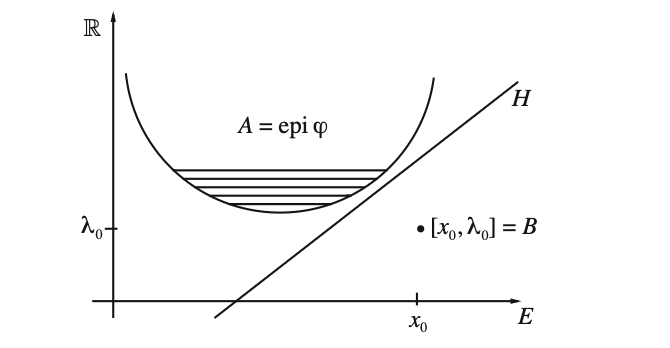
\includegraphics[width=0.8\textwidth]{image/fig2.png}
    \caption{图2}
    \label{fig:2}
\end{figure}

\begin{remark}
显然我们有不等式
\begin{equation}\label{eq11}
\langle f, x \rangle \leq \varphi(x) + \varphi^*(f) \quad \forall x \in E, \quad \forall f \in E^*,
\end{equation}
这有时被称为\textbf{杨氏不等式} (Young's inequality)。当然,这对于$\varphi$的定义是显而易见的!杨氏不等式的经典形式(见第四章定理4.6的证明)断言
\begin{equation}\label{eq12}
ab \leq \frac{1}{p}a^p + \frac{1}{p'}b^{p'} \quad \forall a, b \geq 0
\end{equation}
其中$1 < p < \infty$且$\frac{1}{p}+\frac{1}{p'}=1$。不等式\eqref{eq12}成为\eqref{eq11}的一个特例,其中$E=\mathbb{R}$且$\varphi(t)=\frac{1}{p}|t|^p, \varphi^*(s) = \frac{1}{p'}|s|^{p'}$(见练习1.18, 问题(h))。
\end{remark}

\begin{proposition}\label{proposition1.10}
假设$\varphi: E \to (-\infty, +\infty]$是凸的,l.s.c.的,且$\varphi \not\equiv +\infty$。那么$\varphi^* \not\equiv +\infty$,并且特别地,$\varphi$由一个仿射连续函数从下方有界。
\end{proposition}
\begin{proof}
设$x_0 \in D(\varphi)$并令$\varphi(x_0) < \lambda_0$。我们应用Hahn-Banach(第二几何形式)在空间$E \times \mathbb{R}$中,其中$A = \text{epi } \varphi$,$B = \{[x_0, \lambda_0]\}$。因此,存在一个严格分离$A$和$B$的闭超平面$H=[\Phi=\alpha]$ in $E \times \mathbb{R}$。注意,$\Phi$在$E \times \mathbb{R}$上的每个连续线性泛函都具有形式$\Phi([x, \lambda]) = \langle f, x \rangle + k\lambda$对于某个$f \in E^*$。令$k=\Phi([0,1])$,我们有
\[ \Phi([x, \lambda]) = \langle f, x \rangle + k\lambda \quad \forall [x, \lambda] \in E \times \mathbb{R}. \]
在$A$上写$\Phi > \alpha$,在$B$上写$\Phi < \alpha$,我们得到
\[ \langle f, x \rangle + k\lambda > \alpha \quad \forall [x, \lambda] \in \text{epi } \varphi, \]
和
\[ \langle f, x_0 \rangle + k\lambda_0 < \alpha. \]
特别地,我们有
\begin{equation}\label{eq13}
\langle f, x \rangle + k\varphi(x) > \alpha \quad \forall x \in D(\varphi)
\end{equation}
因此
\[ \langle f, x_0 \rangle + k\varphi(x_0) > \alpha > \langle f, x_0 \rangle + k\lambda_0. \]
它遵循$k>0$。由\eqref{eq13}我们有
\[ \langle -\frac{1}{k}f, x \rangle - \varphi(x) < -\frac{\alpha}{k} \quad \forall x \in D(\varphi) \]
因此$\varphi^*(-\frac{1}{k}f) < +\infty$。
\end{proof}

如果我们迭代操作$*$,我们得到一个在$E^{**}$上定义的函数$\varphi^{**}$。相反,我们选择将其限制在$E$上,我们定义
\[ \varphi^{**}(x) = \sup_{f \in E^*} \{\langle f, x \rangle - \varphi^*(f)\} \quad (x \in E). \]
\begin{theorem}[Fenchel-Moreau]\label{theorem1.11}
设$\varphi: E \to (-\infty, +\infty]$是凸的,l.s.c.的,且$\varphi \not\equiv +\infty$。那么$\varphi^{**}=\varphi$。
\end{theorem}
\begin{proof}
我们分两步进行。
\textbf{步骤1:} 我们另外假设$\varphi \geq 0$并且我们断言$\varphi^{**}=\varphi$。
首先,$\varphi^{**} \leq \varphi$是显然的,因为$\langle f, x \rangle - \varphi^*(f) \leq \varphi(x)$对于所有$x \in E$和$f \in E^*$成立。为了证明$\varphi^{**}=\varphi$,我们通过矛盾来论证,并假设$\varphi^{**}(x_0) < \varphi(x_0)$对于某个$x_0 \in E$成立。如果$\varphi(x_0)=+\infty$,我们可能会有$\varphi^{**}(x_0) < +\infty$,但$\varphi^{**}(x_0)$总是有限的。我们应用定理\ref{theorem1.7}(Hahn-Banach,第二几何形式)在空间$E \times \mathbb{R}$中,其中$A=\text{epi } \varphi$,$B=\{[x_0, \varphi^{**}(x_0)]\}$。所以,存在,如命题\ref{proposition1.10}的证明中那样,一个$f \in E^*$, $k \in \mathbb{R}$和$\alpha \in \mathbb{R}$使得
\begin{gather}
\langle f, x \rangle + k\lambda > \alpha \quad \forall [x, \lambda] \in \text{epi } \varphi, \label{eq14} \\
\langle f, x_0 \rangle + k\varphi^{**}(x_0) < \alpha. \label{eq15}
\end{gather}
它遵循$k \geq 0$(在\eqref{eq14}中令$\lambda \to +\infty$)。[这里我们不能断言,如在命题\ref{proposition1.10}的证明中,$k>0$;我们可能有$k=0$,这将对应于$E \times \mathbb{R}$中的“垂直”超平面$H$。]
让$\varepsilon > 0$;由于$\varphi \geq 0$,我们有,由\eqref{eq14},
\[ \langle f, x \rangle + (k+\varepsilon)\varphi(x) \geq \alpha \quad \forall x \in D(\varphi). \]
因此
\[ \varphi^*\left(-\frac{f}{k+\varepsilon}\right) \leq -\frac{\alpha}{k+\varepsilon}. \]
由$\varphi^{**}$的定义可知
\[ \varphi^{**}(x_0) \geq \left\langle -\frac{f}{k+\varepsilon}, x_0 \right\rangle - \varphi^*\left(-\frac{f}{k+\varepsilon}\right) \geq -\left\langle \frac{f}{k+\varepsilon}, x_0 \right\rangle + \frac{\alpha}{k+\varepsilon}. \]
因此我们有
\[ \langle f, x_0 \rangle + (k+\varepsilon)\varphi^{**}(x_0) \geq \alpha \quad \forall \varepsilon > 0, \]
这与\eqref{eq15}矛盾。

\textbf{步骤2:} 一般情况。
固定一些$f_0 \in D(\varphi^*)$(根据命题\ref{proposition1.10},$D(\varphi^*) \neq \emptyset$)并定义
\[ \bar{\varphi}(x) = \varphi(x) - \langle f_0, x \rangle + \varphi^*(f_0), \]
所以$\bar{\varphi}$是凸的,l.s.c.的,$\bar{\varphi} \not\equiv +\infty$,且$\bar{\varphi} \geq 0$。我们从步骤1知道$(\bar{\varphi})^{**} = \bar{\varphi}$。
让我们现在计算$(\bar{\varphi})^*$和$(\bar{\varphi})^{**}$。我们有
\[ (\bar{\varphi})^*(f) = \varphi^*(f+f_0) - \varphi^*(f_0) \]
和
\[ (\bar{\varphi})^{**}(x) = \varphi^{**}(x) - \langle f_0, x \rangle + \varphi^*(f_0). \]
写$(\bar{\varphi})^{**} = \bar{\varphi}$,我们得到$\varphi^{**} = \varphi$。
\end{proof}

让我们研究一些例子。
\begin{example}
    考虑$\varphi(x) = \|x\|$。很容易检查
\[ \varphi^*(f) = \begin{cases} 0 & \text{如果 } \|f\| \leq 1, \\ +\infty & \text{如果 } \|f\| > 1. \end{cases} \]
由此可知
\[ \varphi^{**}(x) = \sup_{\substack{f \in E^* \\ \|f\| \leq 1}} \langle f, x \rangle. \]
写等式$\varphi^{**}=\varphi$,我们再次获得了推论\ref{corollary1.4}的一部分。
\end{example}

\begin{example}
    给定一个非空集$K \subset E$,我们设
\[ I_K(x) = \begin{cases} 0 & \text{如果 } x \in K, \\ +\infty & \text{如果 } x \notin K. \end{cases} \]
函数$I_K$被称为$K$的\textbf{指示函数} (indicator function)(不应与$K$的特征函数$\chi_K$混淆,后者在$K$上为1,在$K$外为0)。注意,$I_K$是凸的当且仅当$K$是凸集,并且$I_K$是l.s.c.的当且仅当$K$是闭集。$I_K$的共轭函数被称为$K$的\textbf{支撑函数} (supporting function)。很容易看出$I_K^* = I_M$其中$M$是$E^*$的一个子空间,那么$(I_M)^* = I_{M^\perp}$和$(I_M)^{**} = I_{(M^\perp)^\perp}$。假设$M$是一个闭线性子空间并且写$(I_M)^{**} = I_M$,我们得到$(M^\perp)^\perp = M$。在某种意义上,定理\ref{theorem1.11}可以被看作是命题\ref{proposition1.9}的对应物。
我们以另一个有用的共轭函数应用来结束本章。
\end{example}
 

\begin{theorem}[Fenchel-Rockafellar]\label{theorem1.12}
设$\varphi, \psi: E \to (-\infty, +\infty]$是两个凸函数。假设存在某个$x_0 \in D(\varphi) \cap D(\psi)$,使得$\varphi$在$x_0$处是连续的。那么
\[ \inf_{x \in E} \{\varphi(x) + \psi(x)\} = \sup_{f \in E^*} \{-\varphi^*(-f) - \psi^*(f)\} = \max_{f \in E^*} \{-\varphi^*(-f) - \psi^*(f)\} = -\min_{f \in E^*} \{\varphi^*(-f) + \psi^*(f)\}. \]
\end{theorem}
定理\ref{theorem1.12}的证明依赖于下面的引理。
\begin{lemma}\label{lemma1.4}
设$C \subset E$是一个凸集,那么$\text{Int } C$是凸的。\footnote{通常,$\text{Int } C$表示$C$的内部。}此外,如果$\text{Int } C \neq \emptyset$,那么
\[ \bar{C} = \overline{\text{Int } C}. \]
\end{lemma}
为了证明引理\ref{lemma1.4},见,例如,练习1.7。

\begin{proof}
设
\begin{align*}
a &= \inf_{x \in E} \{\varphi(x) + \psi(x)\}, \\
b &= \sup_{f \in E^*} \{-\varphi^*(-f) - \psi^*(f)\}.
\end{align*}
很明显$b \leq a$。如果$a = -\infty$,定理\ref{theorem1.12}的结论是显然的。我们此后假设$a \in \mathbb{R}$。设$C=\text{epi } \varphi$,那么$\text{Int } C \neq \emptyset$(因为$\varphi$在$x_0$处是连续的)。我们应用定理\ref{theorem1.6}(Hahn-Banach,第一几何形式)其中$A=\text{Int } C$和
\[ B = \{[x, \lambda] \in E \times \mathbb{R}; \lambda \leq a-\psi(x)\}. \]
那么$A$和$B$是非空凸集。如果$[x, \lambda] \in A \cap B$,那么$\lambda > \varphi(x)$,另一方面,$\varphi(x) \geq a-\psi(x)$(根据$a$的定义),所以$[x, \lambda] \notin B$。因此$A \cap B = \emptyset$。
因此存在一个分离$A$和$B$的闭超平面$H$。我们从引理\ref{lemma1.4}知道$\bar{A}=\bar{C}$。因此,存在$f \in E^*, k \in \mathbb{R}$和$\alpha \in \mathbb{R}$使得超平面$H = [\Phi = \alpha]$在$E \times \mathbb{R}$中分离$\bar{C}$和$B$,其中
\[ \Phi([x, \lambda]) = \langle f, x \rangle + k\lambda \quad \forall [x, \lambda] \in E \times \mathbb{R}. \]
因此我们有
\begin{gather}
\langle f, x \rangle + k\lambda \geq \alpha \quad \forall [x, \lambda] \in C, \label{eq16} \\
\langle f, x \rangle + k\lambda \leq \alpha \quad \forall [x, \lambda] \in B. \label{eq17}
\end{gather}
在\eqref{eq16}中选择$x=x_0$并令$\lambda \to +\infty$,我们看到$k \geq 0$。我们断言$k>0$。
通过矛盾来假设$k=0$;由此可知$\|f\| \neq 0$(因为$\Phi \not\equiv 0$)。由\eqref{eq16}和\eqref{eq17}我们有
\[ \langle f, x \rangle \geq \alpha \quad \forall x \in D(\varphi), \quad \langle f, x \rangle \leq \alpha \quad \forall x \in D(\psi). \]
但$B(x_0, \varepsilon_0) \subset D(\varphi)$对于某个$\varepsilon_0 > 0$(足够小),因此
\[ \langle f, x_0 + \varepsilon_0 z \rangle \geq \alpha \quad \forall z \in B(0,1), \]
这意味着$\langle f, x_0 \rangle \geq \alpha + \varepsilon_0\|f\|$。另一方面,我们有$\langle f, x_0 \rangle \leq \alpha$,因为$x_0 \in D(\psi)$;因此我们得到$\|f\|=0$,这是一个矛盾,完成了证明。
从\eqref{eq16}和\eqref{eq17}我们得到
\[ \varphi^*\left(-\frac{f}{k}\right) \leq \frac{\alpha}{k} \]
和
\[ \psi^*\left(\frac{f}{k}\right) \leq a - \frac{\alpha}{k}, \]
所以
\[ -\varphi^*\left(-\frac{f}{k}\right) - \psi^*\left(\frac{f}{k}\right) \geq a. \]
另一方面,从$b$的定义,我们有
\[ -\varphi^*\left(-\frac{f}{k}\right) - \psi^*\left(\frac{f}{k}\right) \leq b. \]
我们得出
\[ a=b = -\varphi^*\left(-\frac{f}{k}\right) - \psi^*\left(\frac{f}{k}\right). \]
\end{proof}

\begin{example}
    设$K$是一个非空凸集。我们断言对于每个$x_0 \in E$我们有
\begin{equation}\label{eq19}
\text{dist}(x_0, K) = \inf_{x \in K} \|x-x_0\| = \max_{\substack{f \in E^* \\ \|f\| \leq 1}} \{\langle f, x_0 \rangle - I_K^*(f)\}.
\end{equation}
事实上,我们有
\[ \inf_{x \in K} \|x-x_0\| = \inf_{x \in E} \{\varphi(x) + \psi(x)\} \]
其中$\varphi(x) = \|x-x_0\|$且$\psi(x) = I_K(x)$。应用定理\ref{theorem1.12},我们得到\eqref{eq19}。
在$K=M$是一个线性子空间的特殊情况下,我们得到关系
\[ \text{dist}(x_0, M) = \inf_{x \in M} \|x-x_0\| = \max_{\substack{f \in M^\perp \\ \|f\| \leq 1}} \langle f, x_0 \rangle. \]

\begin{remark}
在$\inf_{x \in K} \|x-x_0\|$未达到的情况下,关系\eqref{eq19}可以为我们提供一些有用的信息(见,例如,练习1.17)。极小曲面理论提供了一个有趣的背景,其中\textbf{原始问题} (primal problem)(即$\inf_{x \in E} \{\varphi(x)+\psi(x)\}$)不必有解,而\textbf{对偶问题} (dual problem)(即$\max_{f \in E^*} \{-\varphi^*(-f)-\psi^*(f)\}$)有解;见I. Ekeland-R. Temam [1]。
\end{remark}
\end{example}

\begin{example}
    设$\varphi: E \to \mathbb{R}$是凸且连续的,并设$M \subset E$是一个线性子空间。那么我们有
\[ \inf_{x \in M} \varphi(x) = -\min_{f \in M^\perp} \varphi^*(f). \]
用$\psi=I_M$应用定理\ref{theorem1.12}就足够了。
\end{example}


	\chapter{一致有界性原理和闭图像定理}

\section{贝尔纲定理}

下面的经典结果在第二章的证明中起着至关重要的作用。

\begin{theorem}[贝尔]\label{theorem2.1}
设$X$是一个完备度量空间,$(X_n)_{n \geq 1}$是$X$中的一列闭子集。假设对于每个$n \geq 1$,
\[
\text{Int } X_n = \emptyset.
\]
那么
\[
\text{Int } \left(\bigcup_{n=1}^\infty X_n\right) = \emptyset.
\]
\end{theorem}

\begin{remark}
贝尔纲定理通常以下面的形式使用。设$X$是一个非空完备度量空间。设$(X_n)_{n \geq 1}$是一列闭子集,使得
\[
\bigcup_{n=1}^\infty X_n = X.
\]
那么存在某个$n_0$使得$\text{Int } X_{n_0} \neq \emptyset$。
\end{remark}

\begin{proof}
令$O_n = X_n^c$,那么对于每个$n \geq 1$,$O_n$在$X$中是开集且稠密。我们的目标是证明$G = \bigcap_{n=1}^\infty O_n$在$X$中是稠密的。设$\omega$是$X$中的一个非空开集;我们将证明$\omega \cap G \neq \emptyset$。
通常,设
\[
B(x, r) = \{y \in X; d(y, x) < r\}.
\]
选择任意$x_0 \in \omega$和$r_0 > 0$使得
\[
\overline{B(x_0, r_0)} \subset \omega.
\]
然后,选择$x_1 \in B(x_0, r_0) \cap O_1$和$r_1 > 0$使得
\[
\begin{cases}
\overline{B(x_1, r_1)} \subset B(x_0, r_0) \cap O_1, \\
0 < r_1 < \frac{r_0}{2},
\end{cases}
\]
这是可能的,因为$O_1$是开集且稠密的。通过归纳,我们构造序列$(x_n)$和$(r_n)$使得
\[
\begin{cases}
\overline{B(x_{n+1}, r_{n+1})} \subset B(x_n, r_n) \cap O_{n+1}, \quad \forall n \geq 0, \\
0 < r_{n+1} < \frac{r_n}{2}.
\end{cases}
\]
由此可知$(x_n)$是一个柯西序列;设$x_n \to \ell$。由于对于每一个$p \geq 0$,$x_{n+p} \in B(x_n, r_n)$,我们在极限(当$p \to \infty$时)得到
\[
\ell \in \overline{B(x_n, r_n)}, \quad \forall n \geq 0.
\]
特别地,$\ell \in \omega \cap G$。
\end{proof}

\section{一致有界性原理}


设$E$和$F$是两个赋范向量空间(n.v.s.)。我们用$\mathcal{L}(E, F)$表示从$E$到$F$的连续(=有界)线性算子的空间,其范数为
\[
\|T\|_{\mathcal{L}(E, F)} = \sup_{\substack{x \in E \\ \|x\| \leq 1}} \|Tx\|.
\]
通常,我们写$\mathcal{L}(E)$而不是$\mathcal{L}(E, E)$。

\begin{theorem}[Banach-Steinhaus, 一致有界性原理]\label{theorem2.2}
设$E$和$F$是两个Banach空间,设$(T_i)_{i \in I}$是从$E$到$F$的一族(不必可数)连续线性算子。假设
\begin{equation}
\sup_{i \in I} \|T_i x\| < \infty \quad \forall x \in E. \label{eq:2.1}
\end{equation}
那么
\begin{equation}
\sup_{i \in I} \|T_i\|_{\mathcal{L}(E, F)} < \infty. \label{eq:2.2}
\end{equation}
换句话说,存在一个常数$c$使得
\[
\|T_i x\| \leq c\|x\| \quad \forall x \in E, \quad \forall i \in I.
\]
\end{theorem}

\begin{remark}
定理\ref{theorem2.2}的结论是相当出人意料和令人惊讶的。从逐点估计可以推导出一个全局(一致)估计。
\end{remark}

\begin{proof}
对于每个$n \geq 1$,令
\[
X_n = \{x \in E; \quad \forall i \in I, \|T_i x\| \leq n\},
\]
所以$X_n$是闭集,并且由\eqref{eq:2.1}我们有
\[
\bigcup_{n=1}^\infty X_n = E.
\]
由贝尔纲定理可知,存在某个$n_0 \geq 1$使得$\text{Int}(X_{n_0}) \neq \emptyset$。选择$x_0 \in E$和$r > 0$使得$B(x_0, r) \subset X_{n_0}$。我们有
\[
\|T_i(x_0+rz)\| \leq n_0 \quad \forall i \in I, \quad \forall z \in B(0, 1).
\]
这导致
\[
r\|T_i\|_{\mathcal{L}(E,F)} \leq n_0 + \|T_i x_0\|,
\]
这意味着\eqref{eq:2.2}成立。
\end{proof}

\begin{remark}
回想一下,连续映射的\textbf{逐点极限}不一定是连续的。线性假设在定理\ref{theorem2.2}中起着至关重要的作用。注意,在定理\ref{theorem2.2}的证明中,我们没有用到$F$是完备的。然而,在下面的设定中,它确实起作用了。
\end{remark}

下面是一致有界性原理的一些直接推论。

\begin{corollary}\label{corollary2.3}
设$E$和$F$是两个Banach空间。设$(T_n)$是从$E$到$F$的一列连续线性算子,使得对于每个$x \in E$,$T_n x$收敛(当$n \to \infty$时)到一个极限,记为$Tx$。那么我们有
\begin{enumerate}[(a)]
\item $\sup_n \|T_n\|_{\mathcal{L}(E,F)} < \infty$,
\item $T \in \mathcal{L}(E,F)$,
\item $\|T\|_{\mathcal{L}(E,F)} \leq \liminf_{n \to \infty} \|T_n\|_{\mathcal{L}(E,F)}$.
\end{enumerate}
\end{corollary}

\begin{proof}
(a) 直接由定理\ref{theorem2.2}得出,因此存在一个常数$c$使得
\[
\|T_n x\| \leq c\|x\| \quad \forall n, \quad \forall x \in E.
\]
在极限处我们发现
\[
\|Tx\| \leq c\|x\| \quad \forall x \in E.
\]
由于$T$显然是线性的,我们得到(b)。
最后,我们有
\[
\|T_n x\| \leq \|T_n\|_{\mathcal{L}(E,F)} \|x\| \quad \forall x \in E,
\]
(c)也直接得出。
\end{proof}

\begin{corollary}\label{corollary2.4}
设$G$是一个Banach空间,设$B$是$G$的一个子集。假设
\begin{equation}
\text{对于每个 } f \in G^*, \text{ 集合 } f(B) = \{\langle f, x \rangle; x \in B\} \text{ 在 } \mathbb{R} \text{ 中是有界的}. \label{eq:2.3}
\end{equation}
那么
\begin{equation}
B \text{ 是有界的}. \label{eq:2.4}
\end{equation}
\end{corollary}

\begin{proof}
我们将使用定理\ref{theorem2.2},其中$E=G^*$, $F=\mathbb{R}$,$I=B$。对于每个$b \in B$,设
\[
T_b(f) = \langle f, b \rangle, \quad f \in E = G^*,
\]
这样由\eqref{eq:2.3},
\[
\sup_{b \in B} |T_b(f)| < \infty \quad \forall f \in E.
\]
由定理\ref{theorem2.2}可知,存在一个常数$c$使得
\[
|\langle f, b \rangle| \leq c\|f\| \quad \forall f \in G^* \quad \forall b \in B.
\]
因此我们发现(使用推论\ref{corollary1.4})
\[
\|b\| \leq c \quad \forall b \in B.
\]
\end{proof}

\begin{remark}
推论\ref{corollary2.4}表明,为了证明一个集合$B$是有界的,只需通过有界线性泛函来“观察”$B$。这是一种在有限维空间中熟悉的过程,其中线性泛函是与某个基相关的分量。在某种意义上,推论\ref{corollary2.4}取代了在无限维空间中的分量使用。有时,人们通过说“弱有界”$\iff$“强有界”来表达推论\ref{corollary2.4}的结论(见第三章)。
\end{remark}

接下来我们有推论\ref{corollary2.4}的一个对偶陈述:

\begin{corollary}\label{corollary2.5}
设$G$是一个Banach空间,设$B^*$是$G^*$的一个子集。假设
\begin{equation}
\text{对于每个 } x \in G, \text{ 集合 } \langle B^*, x \rangle = \{\langle f, x \rangle; f \in B^*\} \text{ 在 } \mathbb{R} \text{ 中是有界的}. \label{eq:2.5}
\end{equation}
那么
\begin{equation}
B^* \text{ 是有界的}. \label{eq:2.6}
\end{equation}
\end{corollary}

\begin{proof}
使用定理\ref{theorem2.2},其中$E=G$, $F=\mathbb{R}$,$I=B^*$。对于每个$b \in B^*$设
\[
T_b(x) = \langle b, x \rangle \quad (x \in G=E).
\]
我们发现存在一个常数$c$使得
\[
|\langle b, x \rangle| \leq c\|x\| \quad \forall b \in B^*, \quad \forall x \in G.
\]
我们得出(从对偶范数的定义)
\[
\|b\| \leq c \quad \forall b \in B^*.
\]
\end{proof}

\section{开映射定理和闭图像定理}

这里是两个由Banach提出的基本结果。

\begin{theorem}[开映射定理]\label{theorem2.6}
设$E$和$F$是两个Banach空间,设$T$是从$E$到$F$的连续线性算子,且$T$是满射的(=映上的)。那么存在一个常数$c>0$使得
\begin{equation}
T(B_E(0,1)) \supset B_F(0,c). \label{eq:2.7}
\end{equation}
\end{theorem}

\begin{remark}
性质\eqref{eq:2.7}意味着$E$中任何开集的像在$F$中是开集(这证明了这个定理的名称!)。确实,让我们假设$U$是$E$中的一个开集,并让我们证明$T(U)$是开的。在$F$中任取一点$y_0 \in T(U)$,设$y_0=Tx_0$对于某个$x_0 \in U$。设$r>0$使得$B(x_0, r) \subset U$,即$x_0+B(0,r) \subset U$。由此可知
\[
y_0 + T(B(0,r)) \subset T(U).
\]
使用\eqref{eq:2.7}我们得到$T(B(0,r)) \supset B(0, rc)$,因此
\[
B(y_0, rc) \subset T(U).
\]
\end{remark}

定理\ref{theorem2.6}的一些重要推论如下。

\begin{corollary}\label{corollary2.7}
设$E$和$F$是两个Banach空间,设$T$是从$E$到$F$的连续线性算子,且$T$是双射的,即单射(=一对一)和满射。那么$T^{-1}$是连续的(从$F$到$E$)。
\end{corollary}

\begin{proof}
推论\ref{corollary2.7}的证明和定理\ref{theorem2.6}的假设立即意味着如果$x \in E$被选择使得$\|Tx\|<c$,那么$\|x\|<1$。通过齐次性,我们有
\[
\|x\| \leq \frac{1}{c} \|Tx\| \quad \forall x \in E
\]
因此$T^{-1}$是连续的。
\end{proof}

\begin{corollary}\label{corollary2.8}
设$E$是一个向量空间,赋有两个范数$\|\cdot\|_1$和$\|\cdot\|_2$。假设$E$对于两个范数都是Banach空间,并且存在一个常数$C \geq 0$使得
\[
\|x\|_2 \leq C\|x\|_1 \quad \forall x \in E.
\]
那么这两个范数是\textbf{等价的},即存在一个常数$c>0$使得
\[
\|x\|_1 \leq c\|x\|_2 \quad \forall x \in E.
\]
\end{corollary}

\begin{proof}
用$E=(E, \|\cdot\|_1)$, $F=(E, \|\cdot\|_2)$和$T=I$来应用推论\ref{corollary2.7}。
\end{proof}

\begin{proof}[定理\ref{theorem2.6}的证明]
我们将证明分为两个步骤。

\textbf{步骤1.} 假设$T$是从$E$到$F$的线性满射算子。那么存在一个常数$c>0$使得
\begin{equation}
\overline{T(B(0,1))} \supset B(0, 2c). \label{eq:2.8}
\end{equation}
\begin{proof}
设$X_n = n\overline{T(B(0,1))}$。由于$T$是满射的,我们有$\bigcup_{n=1}^\infty X_n = F$,并且根据贝尔纲定理,存在某个$n_0$使得$\text{Int}(X_{n_0}) \neq \emptyset$。由此可知
\[
\text{Int}[\overline{T(B(0,1))}] \neq \emptyset.
\]
选择$c>0$和$y_0 \in F$使得
\begin{equation}
B(y_0, 4c) \subset \overline{T(B(0,1))}. \label{eq:2.9}
\end{equation}
特别地,$y_0 \in \overline{T(B(0,1))}$,并且通过对称性,
\begin{equation}
-y_0 \in \overline{T(B(0,1))}. \label{eq:2.10}
\end{equation}
将\eqref{eq:2.9}和\eqref{eq:2.10}相加得到
\[
B(0, 4c) \subset \overline{T(B(0,1))} + \overline{T(B(0,1))}.
\]
另一方面,由于$T(B(0,1))$是凸的,我们有
\[
\overline{T(B(0,1))} + \overline{T(B(0,1))} = 2\overline{T(B(0,1))},
\]
\eqref{eq:2.8}也随之成立。
\end{proof}

\textbf{步骤2.} 假设$T$是从$E$到$F$的连续线性算子,满足\eqref{eq:2.8}。那么我们有
\begin{equation}
T(B(0,1)) \supset B(0,c). \label{eq:2.11}
\end{equation}
\begin{proof}
选择任意$y \in F$使得$\|y\|<c$。我们的目标是找到一个$x \in E$使得
\[
\|x\| < 1 \quad \text{和} \quad Tx=y.
\]
由\eqref{eq:2.8}我们知道
\begin{equation}
\forall \varepsilon > 0 \quad \exists z \in E \text{ with } \|z\| < \frac{1}{2} \text{ and } \|y - Tz\| < \varepsilon. \label{eq:2.12}
\end{equation}
选择$\varepsilon = c/2$,我们找到一些$z_1 \in E$使得
\[
\|z_1\| < \frac{1}{2} \quad \text{和} \quad \|y-Tz_1\| < \frac{c}{2}.
\]
通过对$y-Tz_1$应用与$c/2$(而不是$c$)相同的构造,我们找到一些$z_2 \in E$使得
\[
\|z_2\| < \frac{1}{4} \quad \text{和} \quad \|(y-Tz_1) - Tz_2\| < \frac{c}{4}.
\]
类似地进行,通过归纳我们得到一个序列$(z_n)$使得
\[
\|z_n\| < \frac{1}{2^n} \quad \text{和} \quad \|y-T(z_1+z_2+\dots+z_n)\| < \frac{c}{2^n} \quad \forall n.
\]
由此可知序列$x_n = z_1+z_2+\dots+z_n$是一个柯西序列。设$x_n \to x$,显然,$\|x\| < 1$且$y=Tx$(因为$T$是连续的)。
\end{proof}
\end{proof}

\begin{theorem}[闭图像定理]\label{theorem2.9}
设$E$和$F$是两个Banach空间,设$T$是从$E$到$F$的线性算子。假设$T$的图像$G(T)$在$E \times F$中是闭集。那么$T$是连续的。
\end{theorem}

\begin{remark}
反之亦然,因为任何连续映射的图像都是闭的。
\end{remark}

\begin{proof}
考虑$E$上的两个范数
\[
\|x\|_1 = \|x\|_E + \|Tx\|_F \quad \text{和} \quad \|x\|_2 = \|x\|_E
\]
(范数$\|\cdot\|_1$被称为\textbf{图像范数})。
很容易检查,由于$G(T)$是闭的,$(E, \|\cdot\|_1)$是一个Banach空间。另一方面,$E$也是范数$\|\cdot\|_2$的Banach空间。此外,我们显然有$\|x\|_2 \leq \|x\|_1$。由推论\ref{corollary2.8}可知,这两个范数是等价的,因此存在一个常数$c>0$使得$\|x\|_1 \leq c\|x\|_2$。我们得出$\|Tx\|_F \leq c\|x\|_E$。
\end{proof}

\section{补子空间,线性算子的左右可逆性}

我们从Banach空间中闭子空间的一些几何性质开始,这些性质源于开映射定理。

\begin{theorem}\label{theorem2.10}
设$E$是一个Banach空间。假设$G$和$L$是两个闭线性子空间,使得$G+L$是闭的。那么存在一个常数$C \geq 0$使得
\begin{equation}
\begin{cases}
\text{每个 } z \in G+L \text{ 承认一个形式为} \\
z = x+y \text{ 的分解,其中 } x \in G, y \in L, \text{ 并且 } \|x\| \leq C\|z\| \text{ 和 } \|y\| \leq C\|z\|.
\end{cases} \label{eq:2.13}
\end{equation}
\end{theorem}

\begin{proof}
考虑乘积空间$G \times L$及其范数
\[
\|[x,y]\| = \|x\| + \|y\|
\]
和空间$G+L$及其范数。映射$T: G \times L \to G+L$定义为$T[x,y] = x+y$是连续、线性和满射的。通过开映射定理,存在一个常数$c>0$使得$G+L$中的每个$z$都可以写成$z=x+y$的形式,其中$x \in G, y \in L$且$\|[x,y]\| < c$可以写成$z=x+y$的形式,其中$x \in G, y \in L$且$\|[x,y]\| < c$。通过齐次性,$G+L$中的每个$z$都可以写成
\[
z = x+y \quad \text{其中 } x \in G, y \in L, \text{ 且 } \|x\| + \|y\| \leq (1/c)\|z\|.
\]
\end{proof}

\begin{corollary}\label{corollary2.11}
在与定理\ref{theorem2.10}相同的假设下,存在一个常数$C$使得
\begin{equation}
\text{dist}(x, G \cap L) \leq C\{\text{dist}(x,G) + \text{dist}(x,L)\} \quad \forall x \in E. \label{eq:2.14}
\end{equation}
\end{corollary}

\begin{proof}
给定$x \in E$和$\varepsilon > 0$,存在$a \in G$和$b \in L$使得
\[
\|x-a\| \leq \text{dist}(x,G) + \varepsilon, \quad \|x-b\| \leq \text{dist}(x,L) + \varepsilon.
\]
性质\eqref{eq:2.13}应用于$z=a-b$说明存在$a' \in G$和$b' \in L$使得
\[
a-b = a' + b', \quad \|a'\| \leq C\|a-b\|, \quad \|b'\| \leq C\|a-b\|.
\]
由此可知$a-a' = b+b' \in G \cap L$且
\begin{align*}
\text{dist}(x, G \cap L) &\leq \|x-(a-a')\| \leq \|x-a\| + \|a'\| \\
&\leq \|x-a\| + C\|a-b\| \leq \|x-a\| + C(\|x-a\| + \|x-b\|) \\
&\leq (1+C)\text{dist}(x,G) + \text{dist}(x,L) + (1+2C)\varepsilon.
\end{align*}
最后,我们通过令$\varepsilon \to 0$得到\eqref{eq:2.14}。
\end{proof}

\begin{remark}
推论\ref{corollary2.11}的反命题也成立:如果$G$和$L$是两个闭线性子空间使得\eqref{eq:2.14}成立,那么$G+L$是闭的(见练习2.16)。
\end{remark}

\begin{definition}
设$G \subset E$是Banach空间$E$的一个闭子空间。一个子空间$L \subset E$被称为$G$的\textbf{拓扑补}或简称$G$的\textbf{补},如果
\begin{enumerate}[(i)]
    \item $L$是闭的,
    \item $G \cap L = \{0\}$且$G+L=E$。
\end{enumerate}
我们也说$G$和$L$是$E$的\textbf{互补子空间}。如果成立,那么每个$z \in E$都可以唯一地写成$z=x+y$的形式,其中$x \in G$和$y \in L$。由定理\ref{theorem2.10}可知,投影算子$z \mapsto x$和$z \mapsto y$是连续线性算子。(这个性质也可以作为互补子空间的定义。)
\end{definition}

\begin{example}
\begin{enumerate}
    \item 每个有限维子空间$G$都承认一个补。实际上,设$e_1, e_2, \dots, e_n$是$G$的一个基。$G$中的每个$x$都可以写成$x=\sum_{i=1}^n x_i e_i$。设$\varphi_i(x)=x_i$。使用Hahn-Banach(解析形式)——或者更准确地说是推论\ref{corollary1.2}——每个$\varphi_i$都可以延拓成一个连续线性泛函$\bar{\varphi}_i$定义在$E$上。很容易检查$L = \bigcap_{i=1}^n (\bar{\varphi}_i)^{-1}(0)$是$G$的补。
    \item 每个有限余维的闭子空间$G$都承认一个补。要选择任何与$G \cap L = \{0\}$和$G+L=E$的有限维空间$L$就足够了($L$是闭的,因为它是有限维的)。
    这里是这种情况的一个典型例子。设$N \subset E^*$是$p$维的一个子空间。那么
    \[ G = \{x \in E; \langle f, x \rangle = 0 \quad \forall f \in N\} = N^\perp \]
    是闭的且余维为$p$。实际上,设$f_1, f_2, \dots, f_p$是$N$的一个基。那么存在$e_1, e_2, \dots, e_p \in E$使得
    \[ \langle f_i, e_j \rangle = \delta_{ij} \quad \forall i, j=1, 2, \dots, p. \]
    [考虑映射$\Phi: E \to \mathbb{R}^p$定义为
    \[ \Phi(x) = (\langle f_1, x \rangle, \langle f_2, x \rangle, \dots, \langle f_p, x \rangle) \]
    并注意$\Phi$是满射的;否则,会存在——由Hahn-Banach(第二几何形式)——某个$\alpha=(\alpha_1, \alpha_2, \dots, \alpha_p) \neq 0$使得
    \[ \alpha \cdot \Phi(x) = \sum_{i=1}^n \alpha_i \langle f_i, x \rangle = 0 \quad \forall x \in E, \]
    这是荒谬的]。
    很容易检查由向量$(e_i)_{1 \leq i \leq p}$生成的空间是$G$的线性补。$N^\perp$的余维为$p$的另一个证明是命题\ref{proposition1.11}的事实。
    \item 在希尔伯特空间中,每个闭子空间都承认一个补(见第5.2节)。
\end{enumerate}
\end{example}

\begin{remark}
重要的是要知道一些闭子空间(即使在自反Banach空间中)\textbf{没有补}。事实上,J. Lindenstrauss和L. Tzafriri [1]的一个著名结果断言,在一个Banach空间中,每个闭子空间都承认一个补,当且仅当这个空间与一个希尔伯特空间同构。
\end{remark}

\begin{definition}
设$T \in \mathcal{L}(E,F)$。算子$S \in \mathcal{L}(F,E)$是$T$的\textbf{右逆},如果$T \circ S = I_F$。算子$S \in \mathcal{L}(F,E)$是$T$的\textbf{左逆},如果$S \circ T = I_E$。
\end{definition}

我们的下一个结果为这些逆的存在提供了必要和充分的条件。

\begin{theorem}\label{theorem2.12}
设$T \in \mathcal{L}(E,F)$是\textbf{满射}的。以下性质是等价的:
\begin{enumerate}[(i)]
    \item $T$承认一个右逆。
    \item $N(T) = T^{-1}(0)$在$E$中承认一个补。
\end{enumerate}
\end{theorem}
\begin{proof}
(i) $\implies$ (ii). 设$S$是$T$的一个右逆。很容易看出(请检查)$R(S)=S(F)$是$N(T)$的一个补。

(ii) $\implies$ (i). 设$L$是$N(T)$的一个补。设$P$是从$E$到$L$的(连续)投影算子。给定$f \in F$,我们用$x$表示方程$Tx=f$的任意解。设$S f = Px$并注意$S$独立于$x$的选择。很容易检查$S \in \mathcal{L}(F,E)$且$T \circ S = I_F$。
\end{proof}

\begin{remark}
鉴于注记8和定理\ref{theorem2.12},很容易构造出没有右逆的满射算子$T$。确实,设$G$是一个没有补的闭子空间,并设$F=E/G$,并设$T$是从$E$到$F$的典范投影(关于$E/G$的定义和性质,见第11.2节)。
\end{remark}

\begin{theorem}\label{theorem2.13}
假设$T \in \mathcal{L}(E,F)$是\textbf{单射}的。以下性质是等价的:
\begin{enumerate}[(i)]
    \item $T$承认一个左逆。
    \item $R(T)=T(E)$是闭的并且在$F$中承认一个补。
\end{enumerate}
\end{theorem}
\begin{proof}
(i) $\implies$ (ii). 很容易检查$R(T)$是闭的并且$N(S)$是$R(T)$的补[写$f=TSf+(f-TSf)$]。

(ii) $\implies$ (i). 设$P$是从$F$到$R(T)$的连续投影算子。设$f \in F$;由于$Pf \in R(T)$,存在唯一的$x \in E$使得$Tx=Pf$。设$Sf=x$。很明显$S \circ T = I_E$;此外,根据推论\ref{corollary2.7},$S$是连续的。
\end{proof}


\section{再论正交性}

这里有一些给出和或交的正交表示的简单公式。

\begin{proposition}\label{proposition2.14}
设$G$和$L$是$E$中的两个闭子空间。那么
\begin{gather}
(G \cap L)^\perp = \overline{G^\perp + L^\perp}, \label{eq:2.16} \\
(G+L)^\perp = G^\perp \cap L^\perp. \label{eq:2.17}
\end{gather}
\end{proposition}
\begin{proof}
很明显$G^\perp + L^\perp \subset (G \cap L)^\perp$;因此,如果$x \in (G^\perp+L^\perp)^\perp$并且$f \in G^\perp+L^\perp$那么$\langle f, x \rangle=0$。反之,我们有$G^\perp \subset (G \cap L)^\perp$和$L^\perp \subset (G \cap L)^\perp$。同样地,$(G^\perp+L^\perp)^\perp \subset G \cap L$。因此$(G \cap L)^\perp \supset \overline{G^\perp+L^\perp}$。
\end{proof}

\begin{corollary}\label{corollary2.15}
设$G$和$L$是$E$中的两个闭子空间。那么
\begin{gather}
(G \cap L)^\perp \supset G^\perp+L^\perp, \label{eq:2.18} \\
(G^\perp \cap L^\perp)^\perp = \overline{G+L}. \label{eq:2.19}
\end{gather}
\end{corollary}
\begin{proof}
使用命题\ref{proposition1.9}和\ref{proposition2.14}。
\end{proof}

这里有一个更深的结果。
\begin{theorem}\label{theorem2.16}
设$G$和$L$是Banach空间$E$中的两个闭子空间。以下性质是等价的:
\begin{enumerate}[(a)]
    \item $G+L$在$E$中是闭的,
    \item $G^\perp+L^\perp$在$E^*$中是闭的,
    \item $G+L = (G^\perp \cap L^\perp)^\perp$,
    \item $G^\perp+L^\perp = (G \cap L)^\perp$.
\end{enumerate}
\end{theorem}
\begin{proof}
(a) $\iff$ (c)由\eqref{eq:2.19}得出。(d) $\iff$ (b)是明显的。
我们剩下(a) $\implies$ (d)和(b) $\implies$ (a)的推导。
(a) $\implies$ (d). 鉴于\eqref{eq:2.18}足以证明$(G \cap L)^\perp \subset G^\perp+L^\perp$。给定$f \in (G \cap L)^\perp$,考虑泛函$\varphi: G+L \to \mathbb{R}$定义如下。对于每个$x \in G+L$写$x=a+b$其中$a \in G$和$b \in L$。设
\[ \varphi(x) = \langle f, a \rangle. \]
显然,$\varphi$与$x$的分解无关,且$\varphi$是线性的。另一方面,根据定理\ref{theorem2.10}我们可以选择一种分解$x$的方式使得$\|a\| \leq C\|x\|$,因此
\[ |\varphi(x)| \leq C\|f\| \|x\| \quad \forall x \in G+L. \]
将$\varphi$通过连续线性泛函$\bar{\varphi}$延拓到$E$的所有部分(见推论\ref{corollary1.2})。因此我们有
\[ f = (f-\bar{\varphi}) + \bar{\varphi} \quad \text{其中 } f-\bar{\varphi} \in G^\perp \text{ 且 } \bar{\varphi} \in L^\perp. \]
(b) $\implies$ (a). 我们从推论\ref{corollary2.11}知道存在一个常数$C$使得
\begin{equation}
\text{dist}(f, G^\perp \cap L^\perp) \leq C\{\text{dist}(f, G^\perp) + \text{dist}(f, L^\perp)\} \quad \forall f \in E^*. \label{eq:2.20}
\end{equation}
另一方面,我们有
\begin{equation}
\text{dist}(f, G^\perp) = \sup_{\substack{x \in G \\ \|x\| \leq 1}} \langle f, x \rangle \quad \forall f \in E^*. \label{eq:2.21}
\end{equation}
[使用定理\ref{theorem1.12}其中$\varphi(x)=I_{B_E}(x)-\langle f,x \rangle$和$\psi(x)=I_{G}(x)$,其中
\[ B_E = \{x \in E; \|x\| \leq 1\}.] \]
同样地,我们有
\begin{equation}
\text{dist}(f, L^\perp) = \sup_{\substack{x \in L \\ \|x\| \leq 1}} \langle f, x \rangle \quad \forall f \in E^*. \label{eq:2.22}
\end{equation}
并且由\eqref{eq:2.17})
\begin{equation}
\text{dist}(f, G^\perp \cap L^\perp) = \text{dist}(f, (G+L)^\perp) = \sup_{\substack{x \in G+L \\ \|x\| \leq 1}} \langle f, x \rangle \quad \forall f \in E^*. \label{eq:2.23}
\end{equation}
结合\eqref{eq:2.20}, \eqref{eq:2.21}和\eqref{eq:2.23}我们得到
\begin{equation}
\sup_{\substack{x \in G+L \\ \|x\| \leq 1}} \langle f, x \rangle \leq C \left\{ \sup_{\substack{x \in G \\ \|x\| \leq 1}} \langle f, x \rangle + \sup_{\substack{x \in L \\ \|x\| \leq 1}} \langle f, x \rangle \right\} \quad \forall f \in E^*. \label{eq:2.24}
\end{equation}
由此可知
\begin{equation}
\overline{B_{G+L}} \supset \frac{1}{C} B_{\overline{G+L}}. \label{eq:2.25}
\end{equation}
事实上,通过矛盾来证明,假设存在$x_0 \in \overline{G+L}$其中$\|x_0\| \leq 1/C$且$x_0 \notin \overline{B_G+B_L}$。那么存在一个严格分离$\{x_0\}$和$\overline{B_G+B_L}$的闭超平面。因此存在某个$f_0 \in E^*$和$\alpha \in \mathbb{R}$使得
\[ \langle f_0, x \rangle < \alpha < \langle f_0, x_0 \rangle \quad \forall x \in \overline{B_G+B_L}. \]
因此,我们会有
\[ \sup_{x \in G, \|x\| \leq 1} \langle f_0, x \rangle + \sup_{x \in L, \|x\| \leq 1} \langle f_0, x \rangle \leq \alpha < \langle f_0, x_0 \rangle, \]
这与\eqref{eq:2.24}和\eqref{eq:2.25}的证明相矛盾。
最后,考虑空间$X=G \times L$及其范数
\[ \|[x,y]\| = \max\{\|x\|, \|y\|\} \]
和空间$Y=\overline{G+L}$及其范数。映射$T:X \to Y$定义为$T([x,y])=x+y$是线性和连续的。从\eqref{eq:2.25}我们有
\[ \overline{T(B_X)} \supset \frac{1}{2C} B_Y. \]
使用定理\ref{theorem2.6}(开映射定理)的证明的步骤2我们得出
\[ T(B_X) \supset \frac{1}{2C} B_Y. \]
由此可知$T$从$X$到$Y$是满射的,即$G+L=\overline{G+L}$。
\end{proof}

\section{无界线性算子简介,伴随的定义}

\begin{definition}
设$E$和$F$是两个Banach空间。从$E$到$F$的\textbf{无界线性算子}是一个线性映射$A:D(A) \subset E \to F$定义在一个线性子空间$D(A) \subset E$上,取值在$F$中。$D(A)$被称为$A$的\textbf{定义域}。
如果$D(A)=E$并且存在一个常数$c \geq 0$使得
\[ \|Au\| \leq c\|u\| \quad \forall u \in E. \]
就称$A$是\textbf{有界的}(或\textbf{连续的})。
有界算子的范数定义为
\[ \|A\|_{\mathcal{L}(E,F)} = \sup_{u \neq 0} \frac{\|Au\|}{\|u\|}. \]
\end{definition}

\begin{remark}
当然可能会发生一个无界线性算子结果是有界的。这种术语稍微不一致,但通常被使用并且不会导致混淆。
\end{remark}

这里有一些重要的定义和进一步的记号:
\begin{gather*}
\text{A的图像} = G(A) = \{[u, Au]; u \in D(A)\} \subset E \times F, \\
\text{A的值域} = R(A) = \{Au; u \in D(A)\} \subset F, \\
\text{A的核} = N(A) = \{u \in D(A); Au=0\} \subset E.
\end{gather*}
如果$G(A)$在$E \times F$中是闭的,则称映射$A$是\textbf{闭的}。

\begin{remark}
为了证明一个算子$A$是闭的,一般会进行如下操作。取一个序列$(u_n)$在$D(A)$中使得$u_n \to u$在$E$中且$Au_n \to f$在$F$中。然后检查两个事实:
\begin{enumerate}[(a)]
    \item $u \in D(A)$,
    \item $f=Au$.
\end{enumerate}
注意,仅假设序列$(u_n)$使得$u_n \to 0$在$E$中且$Au_n \to f$在$F$中(并证明$f=0$)是不够的。
\end{remark}

\begin{remark}
如果$A$是闭的,那么$N(A)$是闭的;然而,$R(A)$不一定是闭的。
\end{remark}

\begin{remark}
在实践中,大多数无界算子是\textbf{闭的}并且是\textbf{稠密定义的},即$D(A)$在$E$中是稠密的。
\end{remark}

\begin{definition}
设$A:D(A) \subset E \to F$是一个\textbf{稠密定义}的无界线性算子。我们将引入一个无界线性算子$A^*: D(A^*) \subset F^* \to E^*$。首先,我们定义其定义域:
\[ D(A^*) = \{v \in F^*; \exists c \geq 0 \text{ s.t. } |\langle v, Au \rangle| \leq c\|u\| \quad \forall u \in D(A)\}. \]
\end{definition}

很明显$D(A^*)$是$F^*$的一个线性子空间。我们现在将定义$A^*v$。给定$v \in D(A^*)$,考虑映射$g:D(A) \to \mathbb{R}$定义为
\[ g(u) = \langle v, Au \rangle \quad \forall u \in D(A). \]
我们有
\[ |g(u)| \leq c\|u\| \quad \forall u \in D(A). \]
根据Hahn-Banach(解析形式;见定理\ref{theorem1.1})存在一个线性映射$f:E \to \mathbb{R}$延拓$g$并且使得
\[ |f(u)| \leq c\|u\| \quad \forall u \in E. \]
由此可知$f \in E^*$。注意$g$的延拓是唯一的,因为$D(A)$在$E$中是稠密的。
设
\[ A^*v = f. \]
无界线性算子$A^*:D(A^*) \subset F^* \to E^*$被称为$A$的\textbf{伴随}。简而言之,$A$和$A^*$之间的基本关系由
\[ \langle v, Au \rangle_{F^*,F} = \langle A^*v, u \rangle_{E^*,E} \quad \forall u \in D(A), v \in D(A^*). \]
给出。

\begin{remark}
调用Hahn-Banach来延拓$g$不是必要的。只需使用经典延拓定理,因为$g$在$D(A)$上是一致连续的,并且$E$是完备的(见,例如,H. L. Royden [1](第7章的命题11)或J. Dugundji [1](第XIV章的定理5.2))。
\end{remark}

\begin{remark}
可能会发生$D(A^*)$在$F^*$中不是稠密的(即使$A$是闭的);但这是一个相当病理的情况(见练习2.22)。如果$A$是闭的,则$D(A^*)$在$F^*$的弱$*$拓扑$\sigma(F^*,F)$中总是稠密的(见第三章,问题9)。如果$F$是自反的,那么$D(A^*)$在$F^*$的通常(范数)拓扑中是稠密的(见定理3.24)。
\end{remark}

\begin{remark}
如果$A$是一个有界算子,那么$A^*$也是一个有界算子(从$F^*$到$E^*$)并且此外,
\[ \|A^*\|_{\mathcal{L}(F^*,E^*)} = \|A\|_{\mathcal{L}(E,F)}. \]
确实,很明显$D(A^*)=F^*$。从基本关系,我们有
\[ |\langle A^*v, u \rangle| \leq \|A\| \|v\| \|u\| \quad \forall u \in E, \quad \forall v \in F^*, \]
这意味着$\|A^*v\| \leq \|A\| \|v\|$因此$\|A^*\| \leq \|A\|$。
我们也有
\[ |\langle v, Au \rangle| \leq \|A^*\| \|v\| \|u\| \quad \forall u \in E, \quad \forall v \in F^*, \]
根据推论\ref{corollary1.4},这意味着$\|Au\| \leq \|A^*\|\|u\|$因此$\|A\| \leq \|A^*\|$。
\end{remark}

\begin{proposition}\label{proposition2.17}
设$A:D(A) \subset E \to F$是一个稠密定义的无界线性算子。那么$A^*$是闭的,即$G(A^*)$在$F^* \times E^*$中是闭的。
\end{proposition}
\begin{proof}
设$v_n \in D(A^*)$使得$v_n \to v$在$F^*$中,$A^*v_n \to f$在$E^*$中。我们需要检查(a) $v \in D(A^*)$和(b) $A^*v=f$。
我们有
\[ \langle v_n, Au \rangle = \langle A^*v_n, u \rangle \quad \forall u \in D(A). \]
在极限我们得到
\[ \langle v, Au \rangle = \langle f, u \rangle \quad \forall u \in D(A). \]
因此$v \in D(A^*)$(因为$|\langle v, Au \rangle| \leq \|f\|\|u\| \quad \forall u \in D(A)$)并且$A^*v=f$。
\end{proof}
$A$和$A^*$的图像通过一个非常简单的正交关系相关联:
考虑同构$I:F^* \times E^* \to E^* \times F^*$定义为
\[ I([v,f]) = [-f, v]. \]
设$A:D(A) \subset E \to F$是一个稠密定义的无界线性算子。那么
\[ I[G(A^*)] = G(A)^\perp. \]
确实,设$[v,f] \in F^* \times E^*$,那么
\begin{align*}
[v,f] \in G(A^*) &\iff \langle f,u \rangle = \langle v,Au \rangle \quad \forall u \in D(A) \\
&\iff -\langle f,u \rangle + \langle v,Au \rangle = 0 \quad \forall u \in D(A) \\
&\iff [-f,v] \in G(A)^\perp.
\end{align*}

这里有一些关于值域和核的标准正交关系。
\begin{corollary}\label{corollary2.18}
设$A:D(A) \subset E \to F$是一个稠密定义且闭的无界线性算子。那么
\begin{enumerate}[(i)]
    \item $N(A^*) = R(A)^\perp$,
    \item $N(A) = R(A^*)_\perp$,
    \item $N(A^*)_\perp = \overline{R(A)}$,
    \item $N(A)^\perp = \overline{R(A^*)}$.
\end{enumerate}
\end{corollary}
\begin{proof}
注意(iii)和(iv)直接由(i)和(ii)结合命题\ref{proposition1.9}得出。有一个简单的(i)和(ii)的直接证明(见练习2.18)。然而,通过以下设备将这些事实与命题\ref{proposition2.14}联系起来是有益的。考虑空间$X=E \times F$,那么$X^* = E^* \times F^*$,以及$X$的子空间
\[ G=G(A) \quad \text{和} \quad L=E \times \{0\}. \]
很容易检查
\begin{gather}
N(A) \times \{0\} = G \cap L, \label{eq:2.26} \\
E \times R(A) = G+L, \label{eq:2.27} \\
\{0\} \times N(A^*) = G^\perp \cap L^\perp, \label{eq:2.28} \\
R(A^*) \times F^* = G^\perp + L^\perp. \label{eq:2.29}
\end{gather}
(i)的证明。由\eqref{eq:2.29}我们有
\[ R(A^*) \times \{0\} = (G^\perp+L^\perp) \cap G \cap L \quad \text{(由\eqref{eq:2.16})} \]
\[ = N(A) \times \{0\} \quad \text{(由\eqref{eq:2.26})}. \]
(ii)的证明。由\eqref{eq:2.27}我们有
\[ \{0\} \times R(A)^\perp = (G+L)^\perp = G^\perp \cap L^\perp \quad \text{(由\eqref{eq:2.17})} \]
\[ = \{0\} \times N(A^*) \quad \text{(由\eqref{eq:2.28})}. \]
\end{proof}

\begin{remark}
即使$A$是有界线性算子,也可能发生$N(A) \neq \overline{R(A^*)}$(见练习2.23)。然而,$N(A)^\perp$总是$R(A^*)$在弱$*$拓扑$\sigma(E^*,E)$下的闭包(见问题9)。特别地,如果$E$是自反的,那么$N(A)^\perp = \overline{R(A^*)}$。
\end{remark}

\section{算子的闭值域刻画}
主要结果关注具有闭值域的算子。

\begin{theorem}\label{theorem2.19_again}
设$A:D(A) \subset E \to F$是一个稠密定义且闭的无界线性算子。以下性质是等价的:
\begin{enumerate}[(i)]
    \item $R(A)$是闭的,
    \item $R(A^*)$是闭的,
    \item $R(A) = N(A^*)_\perp$,
    \item $R(A^*) = N(A)^\perp$.
\end{enumerate}
\end{theorem}
\begin{proof}
与推论\ref{corollary2.18}的证明中相同的记号,我们有
\begin{enumerate}[(i)]
    \item $G+L$在$X$中是闭的(见\eqref{eq:2.27}),
    \item $G^\perp+L^\perp$在$X^*$中是闭的(见\eqref{eq:2.29}),
    \item $G+L = (G^\perp \cap L^\perp)^\perp$(见\eqref{eq:2.27}和\eqref{eq:2.28}),
    \item $(G \cap L)^\perp = G^\perp+L^\perp$(见\eqref{eq:2.26}和\eqref{eq:2.29}).
\end{enumerate}
结论则由定理\ref{theorem2.16}得出。
\end{proof}

\begin{remark}
设$A:D(A) \subset E \to F$是一个闭无界线性算子。那么$R(A)$是闭的当且仅当存在一个常数$C$使得
\[ \text{dist}(u, N(A)) \leq C\|Au\| \quad \forall u \in D(A); \]
见练习2.14。
\end{remark}

下一个结果提供了满射算子的一个有用刻画。
\begin{theorem}\label{theorem2.20_again}
设$A:D(A) \subset E \to F$是一个稠密定义的无界线性算子。以下性质是等价的:
\begin{enumerate}[(a)]
    \item $A$是满射的,即$R(A)=F$,
    \item 存在一个常数$C$使得
    \[ \|v\| \leq C\|A^*v\| \quad \forall v \in D(A^*), \]
    (c) $N(A^*) = \{0\}$且$R(A^*)$是闭的。
\end{enumerate}
\end{theorem}
\begin{remark}
(b) $\implies$ (a)的推导有时在建立算子$A$是满射时很有用。一个过程如下。假设$v$满足$A^*v=f$。一个人试图证明$\|v\| \leq C\|f\|$(其中$C$与$f$无关)。这就是所谓的\textbf{先验估计}方法。一个人不关心方程$A^*v=f$是否有解;一个人假设$v$是一个先验解,并试图估计其范数。
\end{remark}
\begin{proof}
(a) $\iff$ (b). 设
\[ B^* = \{v \in D(A^*); \|A^*v\| \leq 1\}. \]
通过齐次性,足以证明$B^*$是有界的。为此——鉴于推论\ref{corollary2.5}(一致有界性原理)——我们只需要证明对于任何$f_0 \in F$集合$\langle B^*, f_0 \rangle$在$\mathbb{R}$中有界。由于$A$是满射的,存在某个$u_0 \in D(A)$使得$Au_0=f_0$。对于每个$v \in B^*$我们有
\[ \langle v, f_0 \rangle = \langle v, Au_0 \rangle = \langle A^*v, u_0 \rangle \]
因此$|\langle v, f_0 \rangle| \leq \|u_0\|$。
(b) $\implies$ (c). 假设$f_n = A^*v_n \to f$。使用(b)我们看到$(v_n)$是柯西序列,所以$v_n \to v$。由于$A^*$是闭的(见命题\ref{proposition2.17}),我们得出$A^*v=f$。
(c) $\implies$ (a). 由于$R(A^*)$是闭的,我们从定理\ref{theorem2.19}推断出$R(A)=N(A^*)_\perp = F$。
\end{proof}

这里有一个“对偶”陈述。
\begin{theorem}\label{theorem2.21_again}
设$A:D(A) \subset E \to F$是一个稠密定义且闭的无界线性算子。以下性质是等价的:
\begin{enumerate}[(a)]
    \item $A^*$是满射的,即$R(A^*)=E^*$,
    \item 存在一个常数$C$使得
    \[ \|u\| \leq C\|Au\| \quad \forall u \in D(A), \]
    (c) $N(A)=\{0\}$且$R(A)$是闭的。
\end{enumerate}
\end{theorem}
\begin{proof}
证明与定理\ref{theorem2.20}的证明类似,我们将其作为一个练习。
\end{proof}
\begin{remark}
如果一个人假设$\dim E < \infty$或$\dim F < \infty$,那么以下是等价的:
\begin{gather*}
A \text{ 满射} \iff A^* \text{ 单射}, \\
A^* \text{ 满射} \iff A \text{ 单射},
\end{gather*}
这确实是有限维空间中线性算子的经典结果。这些等价性成立的原因是$R(A)$和$R(A^*)$是有限维的(因此是闭的)。
在\textbf{一般情况}下,只有以下推论
\begin{gather*}
A \text{ 满射} \implies A^* \text{ 单射}, \\
A^* \text{ 满射} \implies A \text{ 单射}.
\end{gather*}
反例可以从下面的简单例子中看出。设$E=F=\ell^2$;对于每个$x \in \ell^2$写$x=(x_n)_{n \geq 1}$并设$Ax = (\frac{1}{n}x_n)_{n \geq 1}$。很容易看出$A$是一个有界算子且$A^*=A$;$A$(相应地$A^*$)是单射的但$A$(相应地$A^*$)不是满射的;$R(A)$(相应地$R(A^*)$)是稠密的而不是闭的。
\end{remark}



	\chapter{弱拓扑、自反空间、可分空间、一致凸性}

\section{使一族映射连续的最粗拓扑}

我们通过回顾拓扑学中一个著名的概念来开始本章。假设 $X$ 是一个集合(没有任何结构),而 $(Y_i)_{i \in I}$ 是一族拓扑空间。我们给定一族映射 $(\varphi_i)_{i \in I}$,使得对于每个 $i \in I$,$\varphi_i$ 都将 $X$ 映入 $Y_i$。我们考虑以下问题:

\textbf{问题 1.} 在 $X$ 上构造一个拓扑,使得所有映射 $(\varphi_i)_{i \in I}$ 都连续。如果可能,找到一个最经济的拓扑 $\mathcal{T}$,即它拥有\textit{最少的开集}。

注意,如果我们为 $X$ 配备离散拓扑(即 $X$ 的每个子集都是开集),那么每个映射 $\varphi_i$ 都是连续的;当然,这个拓扑远非"最经济的";事实上,它是最昂贵的!我们将看到,总存在一个(唯一的)"最经济的"拓扑 $\mathcal{T}$,使得每个映射 $\varphi_i$ 都连续。它被称为与映射族 $(\varphi_i)_{i \in I}$ 相关联的\textit{最粗拓扑}或\textit{最弱拓扑}(有时也称为\textit{初相拓扑})。

如果 $\omega_i \subset Y_i$ 是任意开集,那么 $\varphi_i^{-1}(\omega_i)$ \textit{必然}是 $\mathcal{T}$ 中的开集。当 $\omega_i$ 取遍 $Y_i$ 的所有开集,并且 $i$ 取遍 $I$ 时,我们得到 $X$ 的一族子集,其中每一个\textit{必须}在拓扑 $\mathcal{T}$ 中是开集。我们用 $(\mathcal{U}_\lambda)_{\lambda \in \Lambda}$ 来表示这个集族。当然,这个集族不一定是一个拓扑。因此,我们引出以下问题:

\textbf{问题 2.} 给定一个集合 $X$ 和 $X$ 的一个子集族 $(\mathcal{U}_\lambda)_{\lambda \in \Lambda}$,在 $X$ 上构造一个最经济的拓扑 $\mathcal{T}$,使得对所有 $\lambda \in \Lambda$,$\mathcal{U}_\lambda$ 都是开集。

换句话说,我们必须找到 $X$ 的子集的最经济的族 $\mathcal{F}$,它在有限交 $\cap_{\text{finite}}$ 和任意并 $\cup_{\text{arbitrary}}$ 下是稳定的\footnote{意为 $\mathcal{F}$ 中有限个集合的交和任意个集合的并都属于 $\mathcal{F}$。},并且具有性质 $\mathcal{U}_\lambda \in \mathcal{F}$ 对所有 $\lambda \in \Lambda$ 成立。构造如下。首先,考虑 $(\mathcal{U}_\lambda)_{\lambda \in \Lambda}$ 中集合的有限交,即 $\cap_{\lambda \in \Gamma} \mathcal{U}_\lambda$,其中 $\Gamma \subset \Lambda$ 是有限的。这样我们得到了一个新的子集族,称为 $\mathcal{B}$,它包含了 $(\mathcal{U}_\lambda)_{\lambda \in \Lambda}$ 并且在 $\cap_{\text{finite}}$ 下是稳定的。然而,它不一定在 $\cup_{\text{arbitrary}}$ 下稳定。因此,我们接下来考虑通过取 $\mathcal{B}$ 中元素的任意并得到的族 $\mathcal{F}$。很明显 $\mathcal{F}$ 在 $\cup_{\text{arbitrary}}$ 下是稳定的。但 $\mathcal{F}$ 是否在 $\cap_{\text{finite}}$ 下稳定并不清楚;但我们确实有以下结果:

\begin{lemma}\label{lemma3.1}
族 $\mathcal{F}$ 在 $\cap_{\text{finite}}$ 下是稳定的。
\end{lemma}

引理 \ref{lemma3.1} 的证明——一个集合论中有趣的练习——留给读者;参见,例如,G. Folland [2]。现在很明显,上述构造给出了具有所需性质的最经济的拓扑。

\begin{remark}\label{remark3.1}
在构造 $\mathcal{T}$ 的过程中,不能颠倒运算的顺序。从 $\cup_{\text{arbitrary}}$ 开始,然后再取 $\cap_{\text{finite}}$ 也是很自然的。其结果是一个在 $\cup_{\text{arbitrary}}$ 下稳定但在 $\cap_{\text{finite}}$ 下不稳定的族。人们将不得不再次考虑 $\cup_{\text{arbitrary}}$,然后过程才会稳定下来。
\end{remark}

总结我们的讨论,我们发现拓扑 $\mathcal{T}$ 的开集是通过首先考虑形如 $\varphi_i^{-1}(\omega_i)$ 的集合的 $\cap_{\text{finite}}$,然后取 $\cup_{\text{arbitrary}}$ 得到的。由此可见,对于每个 $x \in X$,我们通过考虑形如 $\cap_{\text{finite}} \varphi_i^{-1}(V_i)$ 的集合,来获得 $x$ 的一个邻域基,其中 $V_i$ 是 $Y_i$ 中 $\varphi_i(x)$ 的一个邻域。回想一下,在拓扑空间中,点 $x$ 的一个\textit{邻域基}是 $x$ 的一个邻域族,使得 $x$ 的每个邻域都包含该基中的一个邻域。

接下来,我们为 $X$ 配备与映射族 $(\varphi_i)_{i \in I}$ 相关联的最弱拓扑 $\mathcal{T}$。以下是拓扑 $\mathcal{T}$ 的两个简单性质。

\begin{proposition}\label{prop3.1}
设 $(x_n)$ 是 $X$ 中的一个序列。那么 $x_n \to x$(在 $\mathcal{T}$ 中)当且仅当对每个 $i \in I$,$\varphi_i(x_n) \to \varphi_i(x)$。
\end{proposition}

\begin{proof}
如果 $x_n \to x$,那么对每个 $i$,$\varphi_i(x_n) \to \varphi_i(x)$,因为每个 $\varphi_i$ 对 $\mathcal{T}$ 都是连续的。反之,设 $U$ 是 $x$ 的一个邻域。根据前面的讨论,我们总可以假设 $U$ 的形式为 $U = \cap_{j \in J} \varphi_j^{-1}(V_j)$,其中 $J \subset I$ 是有限的。对每个 $j \in J$,存在某个整数 $N_j$ 使得当 $n \ge N_j$ 时,$\varphi_j(x_n) \in V_j$。可以得出,当 $n \ge N = \max_{j \in J} N_j$ 时,$x_n \in U$。
\end{proof}

\begin{proposition}\label{prop3.2}
设 $Z$ 是一个拓扑空间,$\psi$ 是一个从 $Z$ 到 $X$ 的映射。那么 $\psi$ 是连续的当且仅当对每个 $i \in I$,$\varphi_i \circ \psi$ 是从 $Z$ 到 $Y_i$ 的连续映射。
\end{proposition}

\begin{proof}
如果 $\psi$ 是连续的,那么对每个 $i \in I$,$\varphi_i \circ \psi$ 也是连续的。反之,我们必须证明对 $X$ 中的每个开集 $U$,$\psi^{-1}(U)$ 在 $Z$ 中是开集。但我们知道 $U$ 的形式为 $U = \cup_{\text{arbitrary}} \cap_{\text{finite}} \varphi_i^{-1}(\omega_i)$,其中 $\omega_i$ 在 $Y_i$ 中是开集。因此
\[
\psi^{-1}(U) = \bigcup_{\text{arbitrary}} \bigcap_{\text{finite}} \psi^{-1}[\varphi_i^{-1}(\omega_i)] = \bigcup_{\text{arbitrary}} \bigcap_{\text{finite}} (\varphi_i \circ \psi)^{-1}(\omega_i),
\]
它在 $Z$ 中是开集,因为每个映射 $\varphi_i \circ \psi$ 都是连续的。
\end{proof}

\section{弱拓扑 $\sigma(E, E^*)$ 的定义与基本性质}

设 $E$ 是一个 Banach 空间,$f \in E^*$。我们用 $\varphi_f : E \to \mathbb{R}$ 表示线性泛函 $\varphi_f(x) = \langle f, x \rangle$。当 $f$ 遍历 $E^*$ 时,我们得到一族从 $E$ 到 $\mathbb{R}$ 的映射 $(\varphi_f)_{f \in E^*}$。我们现在忽略 $E$ 上通常的拓扑(与 $\| \cdot \|$ 相关联的),并在集合 $E$ 上定义一个新的拓扑如下:

\begin{definition}\label{def_weak_topology}
$E$ 上的\textbf{弱拓扑} $\sigma(E, E^*)$ 是与映射族 $(\varphi_f)_{f \in E^*}$ 相关联的最粗拓扑(在 3.1 节的意义下,其中 $X=E$, $Y_i=\mathbb{R}$ 对每个 $i$ 成立, 且 $I=E^*$)。
\end{definition}

注意,每个映射 $\varphi_f$ 对于通常拓扑都是连续的,因此\textit{弱拓扑比通常拓扑更弱}。

\begin{proposition}\label{prop3.3}
弱拓扑 $\sigma(E, E^*)$ 是 Hausdorff 的。
\end{proposition}

\begin{proof}
给定 $x_1, x_2 \in E$ 且 $x_1 \neq x_2$,我们必须找到弱拓扑 $\sigma(E, E^*)$ 的两个开集 $O_1$ 和 $O_2$,使得 $x_1 \in O_1$,$x_2 \in O_2$,且 $O_1 \cap O_2 = \emptyset$。根据 Hahn-Banach 定理(第二几何形式),存在一个闭超平面严格分离 $\{x_1\}$ 和 $\{x_2\}$。因此,存在某个 $f \in E^*$ 和某个 $\alpha \in \mathbb{R}$ 使得
\[
\langle f, x_1 \rangle < \alpha < \langle f, x_2 \rangle.
\]
令
\begin{align*}
O_1 &= \{ x \in E; \langle f, x \rangle < \alpha \} = \varphi_f^{-1}((-\infty, \alpha)), \\
O_2 &= \{ x \in E; \langle f, x \rangle > \alpha \} = \varphi_f^{-1}((\alpha, +\infty)).
\end{align*}
显然,$O_1$ 和 $O_2$ 对于 $\sigma(E, E^*)$ 是开集,并且它们满足所要求的性质。
\end{proof}

\begin{proposition}\label{prop3.4}
设 $x_0 \in E$;给定 $\varepsilon > 0$ 和 $E^*$ 中的一个\textbf{有限}集 $\{f_1, f_2, \dots, f_k\}$,考虑
\[
V = V(f_1, f_2, \dots, f_k; \varepsilon) = \{x \in E; |\langle f_i, x - x_0 \rangle| < \varepsilon \quad \forall i = 1, 2, \dots, k\}.
\]
则 $V$ 是 $x_0$ 在拓扑 $\sigma(E, E^*)$下的一个邻域。此外,通过改变 $\varepsilon$,$k$ 和 $E^*$ 中的 $f_i$,我们得到了 $x_0$ 在拓扑 $\sigma(E, E^*)$ 下的一个\textbf{邻域基}。
\end{proposition}

\begin{proof}
显然 $V = \cap_{i=1}^k \varphi_{f_i}^{-1}((a_i - \varepsilon, a_i + \varepsilon))$,其中 $a_i = \langle f_i, x_0 \rangle$,因此它在拓扑 $\sigma(E, E^*)$ 中是开集。反之,设 $U$ 是 $x_0$ 在拓扑 $\sigma(E, E^*)$ 下的一个邻域。根据 3.1 节的讨论,我们知道存在一个包含 $x_0$ 的开集 $W \subset U$,其形式为 $W = \cap_{\text{finite} f_i} \varphi_{f_i}^{-1}(\omega_i)$,其中 $\omega_i$ 是 $a_i = \langle f_i, x_0 \rangle$ 在 $\mathbb{R}$ 中的一个邻域。因此存在 $\varepsilon > 0$ 使得对每个 $i$ 都有 $(a_i - \varepsilon, a_i + \varepsilon) \subset \omega_i$。可以得出 $x_0 \in V \subset W \subset U$。
\end{proof}

\textbf{注记.} 如果序列 $(x_n)$ 在弱拓扑 $\sigma(E, E^*)$ 中收敛到 $x$,我们记为
\[ x_n \rightharpoonup x. \]
为避免混淆,我们应说"$x_n \to x$ 在 $\sigma(E, E^*)$ 中弱收敛"。为了完全清楚,我们有时会强调强收敛,说"$x_n \to x$ 强收敛",意为 $\|x_n - x\| \to 0$。

\begin{proposition}\label{prop3.5}
设 $(x_n)$ 是 $E$ 中的一个序列。那么
\begin{itemize}
    \item[(i)] $[x_n \rightharpoonup x \text{ 在 } \sigma(E, E^*) \text{ 中}] \iff [\langle f, x_n \rangle \to \langle f, x \rangle \quad \forall f \in E^*]$。
    \item[(ii)] 如果 $x_n \to x$ 强收敛,则 $x_n \rightharpoonup x$ 在 $\sigma(E, E^*)$ 中弱收敛。
    \item[(iii)] 如果 $x_n \rightharpoonup x$ 在 $\sigma(E, E^*)$ 中弱收敛,则 $(x_n)$ 是有界的,且 $\|x\| \le \liminf \|x_n\|$。
    \item[(iv)] 如果 $x_n \rightharpoonup x$ 在 $\sigma(E, E^*)$ 中弱收敛,且如果 $f_n \to f$ 在 $E^*$ 中强收敛(即 $\|f_n - f\|_{E^*} \to 0)$,则 $\langle f_n, x_n \rangle \to \langle f, x \rangle$。
\end{itemize}
\end{proposition}

\begin{proof}
(i) 直接由弱拓扑 $\sigma(E, E^*)$ 的定义(见命题 \ref{prop3.1})得出。
(ii) 从 (i) 可知,因为 $|\langle f, x_n \rangle - \langle f, x \rangle| = |\langle f, x_n - x \rangle| \le \|f\| \|x_n - x\|$。
(iii) 由一致有界性原理(见推论 \ref{corollary2.4})可知,对于每个 $f \in E^*$,序列 $(\langle f, x_n \rangle)_n$ 是有界的。对不等式取极限
\[ |\langle f, x_n \rangle| \le \|f\| \|x_n\|, \]
我们得到
\[ |\langle f, x \rangle| \le \|f\| \liminf \|x_n\|, \]
这(根据推论 \ref{corollary1.4})意味着
\[ \|x\| = \sup_{\|f\| \le 1} |\langle f, x \rangle| \le \liminf \|x_n\|. \]
(iv) 由不等式
\[ |\langle f_n, x_n \rangle - \langle f, x \rangle| \le |\langle f_n - f, x_n \rangle| + |\langle f, x_n - x \rangle| \le \|f_n - f\|_{E^*} \|x_n\| + |\langle f, x_n - x \rangle|, \]
结合 (i) 和 (iii) 可得。
\end{proof}

\begin{proposition}\label{prop3.6}
当 $E$ 是\textbf{有限维}空间时,弱拓扑 $\sigma(E, E^*)$ 和通常拓扑是\textbf{相同}的。因此,一个序列弱收敛当且仅当它强收敛。
\end{proposition}

\begin{proof}
因为弱拓扑的开集\textit{总是}比强拓扑少,所以它足以证明每个强开集也是弱开集。设 $x_0 \in E$ 且 $U$ 是 $x_0$ 在强拓扑中的一个邻域。我们必须找到一个 $x_0$ 在弱拓扑 $\sigma(E, E^*)$ 中的邻域 $V$ 使得 $V \subset U$。换句话说,我们要找到 $f_1, f_2, \dots, f_k \in E^*$ 和 $\varepsilon > 0$ 使得
\[ V = \{x \in E; |\langle f_i, x - x_0 \rangle| < \varepsilon \quad \forall i = 1, 2, \dots, k\} \subset U. \]
不妨假设 $U$ 是球 $B(x_0, r)$。选择 $E$ 的一个基 $e_1, e_2, \dots, e_k$ 使得 $\|e_i\|=1$ 对所有 $i$ 成立。$E$ 中的每个 $x$ 都可以分解为 $x = \sum_{i=1}^k x_i e_i$,并且映射 $x \mapsto x_i$ 是 $E$ 上的连续线性泛函。我们有
\[ \|x - x_0\| \le \sum_{i=1}^k |x_i - (x_0)_i| \|e_i\| < k\varepsilon \]
对于每个 $x \in V$。选择 $\varepsilon = r/k$,我们得到 $V \subset U$。
\end{proof}

\begin{remark}\label{remark3.2}
在弱拓扑 $\sigma(E, E^*)$ 中的开集(闭集)在强拓扑中也总是开集(闭集)。在\textbf{无限维}空间中,弱拓扑\textbf{严格}比强拓扑粗糙;即,存在在强拓扑中是开集(闭集)但在弱拓扑中不是开集(闭集)的集合。以下是两个例子:
\end{remark}

\textbf{例 1.} 单位球面 $S = \{x \in E; \|x\| = 1\}$,当 $E$ 是无限维时,在弱拓扑 $\sigma(E, E^*)$ 中\textbf{永不}闭。更精确地说,我们有
\begin{equation}\label{eq:weak_closure_sphere}
\overline{S}^{\sigma(E, E^*)} = B_E,
\end{equation}
其中 $\overline{S}^{\sigma(E, E^*)}$ 表示 $S$ 在 $\sigma(E, E^*)$ 中的闭包,而 $B_E$ 表示 $E$ 中的闭单位球,
\[ B_E = \{x \in E; \|x\| \le 1\}. \]
为了完成 (\ref{eq:weak_closure_sphere}) 的证明,只需知道 $B_E$ 在 $\sigma(E, E^*)$ 中是闭的。但我们有
\[ B_E = \bigcap_{f \in E^*, \|f\| \le 1} \{x \in E; |\langle f, x \rangle| \le 1\}, \]
它是弱闭集的交集。

\textbf{例 2.} 单位开球 $U = \{x \in E; \|x\| < 1\}$,当 $E$ 是无限维时,在弱拓扑 $\sigma(E, E^*)$ 中\textbf{永不}开。假设与此相反,$U$ 是弱开的。那么它的补集 $U^c = \{x \in E; \|x\| \ge 1\}$ 将是弱闭的。它表明 $S = B_E \cap U^c$ 也是弱闭的,这与例 1 相矛盾。

\begin{remark}\label{remark3.3}
在无限维空间中,弱拓扑是\textbf{不可度量}的,即,不存在一个范数(或更一般的,一个度量)能够诱导出 $\sigma(E, E^*)$ 拓扑;见练习 3.8。然而,正如我们将在定理 \ref{theorem3.29} 中看到的,如果 $E^*$ 是可分的,人们可以在 $E$ 的有界集上定义一个范数,它在这些集合上诱导出弱拓扑 $\sigma(E, E^*)$。
\end{remark}

\begin{remark}\label{remark3.4}
通常,在无限维空间中,存在弱收敛但不强收敛的序列。如果 $E^*$ 是可分的或 $E$ 是自反的(见练习 3.22),人们可以构造一个序列 $(x_n)$ 在 $E$ 中,使得 $\|x_n\| = 1$ 对所有 $n$ 成立且 $x_n \rightharpoonup 0$ 弱收敛。然而,在具有性质每个有界序列都有弱收敛子序列的无限维空间中,弱拓扑严格比强拓扑粗糙。这些序列是相当"罕见"和有些"病态"的。这个奇怪的事实与注记 \ref{remark3.2} 并不矛盾,后者断言在无限维空间中,弱拓扑严格比强拓扑粗糙,因为即使两个拓扑具有相同的收敛序列,它们也未必是两个相同的拓扑。
\end{remark}

\section{弱拓扑、凸集与线性算子}

每个弱闭集都是强闭的,但在无限维空间中,反之则为假(见注记 \ref{remark3.2})。然而,对于凸集来说,弱闭=强闭,这是非常有用的。

\begin{theorem}\label{theorem3.7}
设 $C$ 是 $E$ 的一个凸子集。那么 $C$ 在弱拓扑 $\sigma(E, E^*)$ 中是闭的当且仅当它在强拓扑中是闭的。
\end{theorem}

\begin{proof}
假设 $C$ 在强拓扑中是闭的,我们来证明 $C$ 在弱拓扑中也是闭的。为此,我们只需证明其补集 $C^c$ 在弱拓扑中是开的。设 $x_0 \notin C$。由 Hahn-Banach 定理,存在一个闭超平面严格分离 $\{x_0\}$ 和 $C$。因此,存在某个 $f \in E^*$ 和某个 $\alpha \in \mathbb{R}$ 使得
\[ \langle f, x_0 \rangle < \alpha < \langle f, y \rangle \quad \forall y \in C. \]
设
\[ V = \{x \in E; \langle f, x \rangle < \alpha \}, \]
那么 $x_0 \in V$, $V \cap C^c = \emptyset$(即,$V \subset C^c$)并且 $V$ 在弱拓扑中是开的。
\end{proof}

\begin{corollary}[Mazur]\label{corollary3.8}
假设 $(x_n)$ 弱收敛到 $x$。那么存在一个由 $x_n$ 的凸组合构成的序列 $(y_n)$,它强收敛到 $x$。
\end{corollary}

\begin{proof}
设 $C = \text{conv}(\cup_{p=1}^\infty \{x_p\})$ 表示 $x_n$ 的凸包。由于 $x$ 属于 $\cup_{p=1}^\infty \{x_p\}$ 的弱闭包,它也先验地属于 $C$ 的弱闭包。根据定理 \ref{theorem3.7},$x \in \bar{C}$,即 $C$ 的强闭包,结论由此得出。
\end{proof}

\begin{theorem}\label{theorem3.10}
设 $E$ 和 $F$ 是两个 Banach 空间,$T$ 是一个从 $E$ 到 $F$ 的线性算子。假设 $T$ 在强拓扑下是连续的。那么 $T$ 在弱拓扑 $\sigma(E, E^*)$ 和 $\sigma(F, F^*)$ 下也是连续的,反之亦然。
\end{theorem}

\begin{proof}
根据命题 \ref{prop3.2} 的观点,只需验证对每个 $f \in F^*$,映射 $x \mapsto \langle f, Tx \rangle$ 是从 $E$ 映入 $\mathbb{R}$ 的连续映射。但映射 $x \mapsto \langle f, Tx \rangle$ 是 $E$ 上的一个连续线性泛函。它也因此在弱拓扑 $\sigma(E, E^*)$ 中连续。
\end{proof}

\section{弱*拓扑 $\sigma(E^*, E)$}

到目前为止,我们有两种拓扑:
\begin{itemize}
    \item[(a)] 与 $E^*$ 的范数相关的(强)拓扑
    \item[(b)] 弱拓扑 $\sigma(E^*, E^{**})$,通过第 3.3 节的构造得到
\end{itemize}

我们现在要定义 $E^*$ 上的\textbf{第三种}拓扑,称为\textbf{弱*拓扑},记为 $\sigma(E^*, E)$(这里的 $*$ 是为了提醒我们这是在对偶空间上定义的)。对于每个 $x \in E$,我们考虑线性泛函 $\varphi_x: E^* \to \mathbb{R}$,定义为 $\varphi_x(f) = \langle f, x \rangle$。这样,我们从 $E^*$ 到 $\mathbb{R}$ 得到了一族映射 $(\varphi_x)_{x \in E}$。

\begin{definition}\label{def_weak_star_topology}
$E^*$ 上的\textbf{弱*拓扑} $\sigma(E^*, E)$ 是与映射族 $(\varphi_x)_{x \in E}$ 相关联的最粗拓扑(在 3.1 节的意义下,其中 $X = E^*$,$Y_i = \mathbb{R}$ 对所有 $i$ 成立,且 $I = E$)。
\end{definition}

由于 $E \subset E^{**}$,显然拓扑 $\sigma(E^*, E)$ 比拓扑 $\sigma(E^*, E^{**})$ 更粗糙;即,$\sigma(E^*, E)$ 的开集(相应地,闭集)比 $\sigma(E^*, E^{**})$ 少,后者又比强拓扑的开集(闭集)少。

\begin{remark}\label{remark3.8}
读者可能会想,为什么会有这种对拓扑的歇斯底里。原因是:\textit{一个更粗糙的拓扑有更多的紧集}。例如,闭单位球 $B_{E^*}$ 在强拓扑中\textit{永不}紧(除非 dim $E < \infty$);见定理 \ref{theorem:6.5}。了解紧集的基本作用——例如,在存在性机制中,如最小化问题——对于理解弱*拓扑的重要性至关重要。
\end{remark}

\begin{proposition}\label{prop3.11}
弱*拓扑是 Hausdorff 的。
\end{proposition}

\begin{proof}
给定 $f_1, f_2 \in E^*$ 且 $f_1 \neq f_2$,存在某个 $x \in E$ 使得 $\langle f_1, x \rangle \neq \langle f_2, x \rangle$(这不需要 Hahn-Banach,仅仅是 $f_1 \neq f_2$ 的事实)。例如,假设 $\langle f_1, x \rangle < \langle f_2, x \rangle$ 并选择一个 $\alpha$ 使得
\[ \langle f_1, x \rangle < \alpha < \langle f_2, x \rangle. \]
令
\begin{align*}
O_1 &= \{ f \in E^*; \langle f, x \rangle < \alpha \} = \varphi_x^{-1}((-\infty, \alpha)), \\
O_2 &= \{ f \in E^*; \langle f, x \rangle > \alpha \} = \varphi_x^{-1}((\alpha, +\infty)).
\end{align*}
则 $O_1$ 和 $O_2$ 是 $\sigma(E^*, E)$ 中的开集,使得 $f_1 \in O_1, f_2 \in O_2$ 且 $O_1 \cap O_2 = \emptyset$。
\end{proof}

\begin{proposition}\label{prop3.12}
设 $f_0 \in E^*$;给定一个有限集 $\{x_1, x_2, \dots, x_k\}$ 在 $E$ 中和 $\varepsilon > 0$,考虑
\[ V = V(x_1, x_2, \dots, x_k; \varepsilon) = \{f \in E^*; |\langle f - f_0, x_i \rangle| < \varepsilon \quad \forall i = 1, 2, \dots, k\}. \]
那么 $V$ 是 $f_0$ 在拓扑 $\sigma(E^*, E)$ 下的一个邻域。此外,我们通过改变 $\varepsilon$,$k$ 和 $E$ 中的 $x_i$ 得到了 $f_0$ 在 $\sigma(E^*, E)$ 下的一个\textbf{邻域基}。
\end{proposition}

\begin{proof}
与命题 \ref{prop3.4} 的证明相同。
\end{proof}

\textbf{注记.} 如果一个序列 $(f_n)$ 在弱*拓扑中收敛于 $f$,我们记为
\[ f_n \stackrel{*}{\rightharpoonup} f. \]
为避免混淆,我们有时会强调 $"f_n \stackrel{*}{\rightharpoonup} f$ 在 $\sigma(E^*, E)$ 中"。

\begin{proposition}\label{prop3.13}
设 $(f_n)$ 是 $E^*$ 中的一个序列。那么
\begin{itemize}
    \item[(i)] $[f_n \stackrel{*}{\rightharpoonup} f \text{ in } \sigma(E^*, E)] \iff [\langle f_n, x \rangle \to \langle f, x \rangle \quad \forall x \in E]$。
    \item[(ii)] 如果 $f_n \to f$ 强收敛,那么 $f_n \stackrel{*}{\rightharpoonup} f$ 在 $\sigma(E^*, E)$ 中。
    \item[(iii)] 如果 $f_n \stackrel{*}{\rightharpoonup} f$ 在 $\sigma(E^*, E)$ 中,那么 $(f_n)$ 是有界的,且 $\|f\| \le \liminf \|f_n\|$。
    \item[(iv)] 如果 $f_n \stackrel{*}{\rightharpoonup} f$ 在 $\sigma(E^*, E)$ 中,且如果 $x_n \to x$ 强收敛在 $E$ 中,那么 $\langle f_n, x_n \rangle \to \langle f, x \rangle$。
\end{itemize}
复制命题 \ref{prop3.5} 的证明。
\end{proposition}

\begin{remark}\label{remark3.9}
假设 $f_n \stackrel{*}{\rightharpoonup} f$ 在 $\sigma(E^*, E)$ 中(甚至 $f_n \to f$ 在 $\sigma(E^*, E^{**})$ 中)且 $x_n \rightharpoonup x$ 在 $\sigma(E, E^*)$ 中。通常情况下,我们不能断言 $\langle f_n, x_n \rangle \to \langle f, x \rangle$(在 Hilbert 空间中构造一个反例非常容易)。
\end{remark}

\begin{remark}\label{remark3.10}
当 $E$ 是有限维空间时,三种拓扑(强、弱、弱*)在 $E^*$ 上是一致的。事实上,典范映射 $J: E \to E^{**}$ 是满射的(因为 $\dim E = \dim E^{**}$),因此 $\sigma(E^*, E) = \sigma(E^*, E^{**})$。
\end{remark}

\begin{proposition}\label{prop3.14}
设 $\varphi: E^* \to \mathbb{R}$ 是一个对于弱*拓扑连续的线性泛函。那么存在某个 $x_0 \in E$ 使得
\[ \varphi(f) = \langle f, x_0 \rangle \quad \forall f \in E^*. \]
\end{proposition}

该证明依赖于以下有用的代数引理:
\begin{lemma}\label{lemma3.2}
设 $X$ 是一个向量空间,$\varphi, \varphi_1, \varphi_2, \dots, \varphi_k$ 是 $X$ 上的 $(k+1)$ 个线性泛函,使得
\begin{equation}\label{eq:lemma3.2_cond}
[\varphi_i(v) = 0 \quad \forall i = 1, 2, \dots, k] \implies [\varphi(v) = 0].
\end{equation}
那么存在常数 $\lambda_1, \lambda_2, \dots, \lambda_k \in \mathbb{R}$ 使得 $\varphi = \sum_{i=1}^k \lambda_i \varphi_i$。
\end{lemma}

\begin{proof}
考虑映射 $F: X \to \mathbb{R}^{k+1}$ 定义为
\[ F(u) = [\varphi(u), \varphi_1(u), \dots, \varphi_k(u)]. \]
由假设 (\ref{eq:lemma3.2_cond}) 可知,点 $a = [1, 0, 0, \dots, 0]$ 不属于 $R(F)$。因此,我们可以严格地分离 $\{a\}$ 和 $R(F)$;即,存在 $\mathbb{R}^{k+1}$ 中的常数 $\lambda, \lambda_1, \dots, \lambda_k$ 和 $\alpha$ 使得
\[ \lambda < \alpha < \lambda \varphi(u) + \sum_{i=1}^k \lambda_i \varphi_i(u) \quad \forall u \in X. \]
由此得出
\[ \lambda \varphi(u) + \sum_{i=1}^k \lambda_i \varphi_i(u) = 0 \quad \forall u \in X \]
并且 $\lambda < 0$ (所以 $\lambda \neq 0$)。
\end{proof}

\begin{proof}
由于 $\varphi$ 在弱*拓扑 $\sigma(E^*, E)$ 下是连续的,所以存在一个 $0$ 的邻域 $V$ 使得
\[ |\varphi(f)| < 1 \quad \forall f \in V. \]
我们总可以假设
\[ V = \{ f \in E^*; |\langle f, x_i \rangle| < \varepsilon \quad \forall i = 1, 2, \dots, k \} \]
对于某些 $x_i \in E$ 和 $\varepsilon > 0$。特别地,
\[ [\langle f, x_i \rangle = 0 \quad \forall i = 1, \dots, k] \implies [\varphi(f)=0]. \]
\end{proof}

\begin{corollary}\label{corollary3.15}
假设 $H$ 是 $E^*$ 中在 $\sigma(E^*, E)$ 下闭的超平面。那么 $H$ 具有形式
\[ H = \{f \in E^*; \langle f, x_0 \rangle = \alpha\} \]
对于某个 $x_0 \in E$, $x_0 \neq 0$, 和某个 $\alpha \in \mathbb{R}$。
\end{corollary}

\section{自反空间}

\begin{definition}\label{def_reflexive_space}
设 $E$ 是一个 Banach 空间,$J: E \to E^{**}$ 是典范注入(见 1.3 节)。如果 $J$ 是满射的,即 $J(E) = E^{**}$,则称空间 $E$ 是\textbf{自反的}。
\end{definition}

当 $E$ 是自反的时,$E^{**}$ 通常与 $E$ 等同。显然,有限维空间是自反的(因为 $\dim E = \dim E^* = \dim E^{**}$)。我们将在第四章(亦见第十一章)看到,如果 $1 < p < \infty$,$L^p$(和 $\ell^p$)空间是自反的。然而,希尔伯特空间是自反的。然而,一些重要的空间不是自反的:
\begin{itemize}
    \item $L^1$ 和 $L^\infty$ (以及 $\ell^1, \ell^\infty$)不是自反的(见第四章和第十一章)。
    \item $C(K)$,在一个无限紧致度量空间 $K$ 上的连续函数空间,不是自反的(见练习 3.25)。
\end{itemize}

\begin{theorem}[Banach-Alaoglu-Bourbaki]\label{theorem3.16}
$B_{E^*} = \{f \in E^*; \|f\| \le 1\}$ 在弱*拓扑 $\sigma(E^*, E)$ 中是紧的。
\end{theorem}

\begin{remark}\label{remark3.12}
$B_{E^*}$ 的紧性是弱*拓扑\textit{最重要}的性质;亦见注记 \ref{remark3.8}。
\end{remark}

\begin{proof}
考虑笛卡尔积 $Y = \mathbb{R}^E$,它由所有从 $E$ 到 $\mathbb{R}$ 的映射组成;我们用 $\omega = (\omega_x)_{x \in E}$ 来表示 $Y$ 的元素,其中 $\omega_x \in \mathbb{R}$。空间 $Y$ 配备了乘积拓扑。根据 Tychonoff 定理,这个空间是紧的。现在,考虑从 $E^*$ 到 $Y$ 的典范注入 $\Phi$,定义为 $\Phi(f) = (\langle f, x \rangle)_{x \in E}$。清楚地,$\Phi$ 是从 $E^*$(配备弱*拓扑 $\sigma(E^*, E)$)到 $\Phi(E^*) \subset Y$(配备 $Y$ 的拓扑)的一个同胚。另一方面,很清楚 $\Phi(B_{E^*}) = K$,其中 $K$ 是一个紧集。
\[
K = \left\{ \omega \in Y \middle| 
\begin{aligned}
&|\omega_x| \le \|x\|, \quad \omega_{x+y} = \omega_x + \omega_y \\
&\text{和 } \omega_{\lambda x} = \lambda \omega_x \quad \forall x, y \in E, \forall \lambda \in \mathbb{R}
\end{aligned}
\right\}.
\]
为了完成定理 \ref{theorem3.16} 的证明,只需证明 $K$ 是 $Y$ 的一个紧子集。将 $K$ 写成 $K=K_1 \cap K_2$,其中
\[ K_1 = \{\omega \in Y; |\omega_x| \le \|x\| \quad \forall x \in E\} \]
和
\[ K_2 = \{\omega \in Y; \omega_{x+y} = \omega_x + \omega_y \text{ 和 } \omega_{\lambda x} = \lambda \omega_x \quad \forall \lambda \in \mathbb{R}, x, y \in E \}. \]
集合 $K_1$ 也可以写成闭区间的乘积
\[ K_1 = \prod_{x \in E} [-\|x\|, +\|x\|]. \]
让我们回顾一下,紧空间的任意乘积是紧的——一个深邃的定理,归功于 Tychonoff;见,例如,H. L. Royden [1], G. B. Folland [2], J. R. Munkres [1]。因此 $K_1$ 是紧的。另一方面, $K_2$ 在 $Y$ 中是闭的;确实,为每个固定的 $\lambda \in \mathbb{R}, x, y \in E$ 定义集合
\begin{align*}
    A_{x,y} &= \{\omega \in Y; \omega_{x+y} - \omega_x - \omega_y = 0\}, \\
    B_{\lambda,x} &= \{\omega \in Y; \omega_{\lambda x} - \lambda\omega_x = 0\},
\end{align*}
它们在 $Y$ 中是闭的(因为映射 $\omega \mapsto \omega_{x+y} - \omega_x - \omega_y$ 和 $\omega \mapsto \omega_{\lambda x} - \lambda\omega_x$ 在 $Y$ 上是连续的),并且我们有
\[ K_2 = \left[ \bigcap_{x,y \in E} A_{x,y} \right] \cap \left[ \bigcap_{\substack{x \in E \\ \lambda \in \mathbb{R}}} B_{\lambda,x} \right]. \]
最后, $K$ 是紧的,因为它是紧集 ($K_1$) 和闭集 ($K_2$) 的交集。
\end{proof}

\begin{theorem}[Kakutani]\label{theorem3.17}
设 $E$ 是一个 Banach 空间。那么 $E$ 是自反的当且仅当
\[ B_E = \{x \in E; \|x\| \le 1\} \]
在弱拓扑 $\sigma(E, E^*)$ 中是紧的。
\end{theorem}

\begin{proof}
假设 $E$ 是自反的,那么 $J(B_E) = B_{E^{**}}$。我们已经知道(由定理 \ref{theorem3.16})$B_{E^{**}}$ 在拓扑 $\sigma(E^{**}, E^*)$ 中是紧的。因此,要证明 $J^{-1}$ 在配备 $\sigma(E^{**}, E^*)$ 拓扑的 $E^{**}$ 和配备 $\sigma(E, E^*)$ 拓扑的 $E$ 之间是连续的就足够了。根据命题 \ref{prop3.2} 的观点,我们只需验证对于每个固定的 $f \in E^*$,映射 $\xi \mapsto \langle f, J^{-1}\xi \rangle$ 在配备了 $\sigma(E^{**}, E^*)$ 拓扑的 $E^{**}$ 上是连续的。但 $\langle f, J^{-1}\xi \rangle = \langle \xi, f \rangle$,并且映射 $\xi \mapsto \langle \xi, f \rangle$ 确实是 $\sigma(E^{**}, E^*)$ 拓扑的定义元素之一。因此我们已经证明了 $B_E$ 在 $\sigma(E, E^*)$ 中是紧的。

反向证明更为精细,依赖于以下两个引理:

\end{proof}
\begin{lemma}[Helly]\label{lemma3.3}
设 $E$ 是一个 Banach 空间。给定 $E^*$ 中的 $f_1, f_2, \dots, f_k$ 和 $\mathbb{R}$ 中的 $\gamma_1, \gamma_2, \dots, \gamma_k$。以下性质是等价的:
\begin{itemize}
    \item[(i)] $\forall \varepsilon > 0 \quad \exists x_\varepsilon \in E$ 使得 $\|x_\varepsilon\| \le 1$ 并且
    \[ |\langle f_i, x_\varepsilon \rangle - \gamma_i| < \varepsilon \quad \forall i=1, 2, \dots, k, \]
    \item[(ii)] $|\sum_{i=1}^k \beta_i \gamma_i| \le \|\sum_{i=1}^k \beta_i f_i\|$ 对所有 $\beta_1, \beta_2, \dots, \beta_k \in \mathbb{R}$ 和 $S = \sum_{i=1}^k |\beta_i|$。
\end{itemize}
\end{lemma}

\begin{proof}
(i) $\implies$ (ii)。固定 $\beta_1, \beta_2, \dots, \beta_k \in \mathbb{R}$ 并令 $S = \sum_{i=1}^k |\beta_i|$。由 (i) 可知
\[ |\sum_{i=1}^k \beta_i (\langle f_i, x_\varepsilon \rangle - \gamma_i)| \le \varepsilon S \]
因此
\[ |\sum_{i=1}^k \beta_i \gamma_i| \le |\sum_{i=1}^k \beta_i \langle f_i, x_\varepsilon \rangle| + \varepsilon S \le \|\sum_{i=1}^k \beta_i f_i\| + \varepsilon S. \]
由于这对任意 $\varepsilon > 0$ 成立,我们得到 (ii)。

(ii) $\implies$ (i)。设 $\gamma = (\gamma_1, \dots, \gamma_k) \in \mathbb{R}^k$ 并考虑映射 $\varphi: E \to \mathbb{R}^k$ 定义为
\[ \varphi(x) = ((\langle f_1, x \rangle, \dots, (\langle f_k, x \rangle)). \]
性质 (i) 表示 $\gamma \in \overline{\varphi(B_E)}$。假设与此相反,$\gamma \notin \overline{\varphi(B_E)}$。那么 $\{\gamma\}$ 和 $\overline{\varphi(B_E)}$ 可以被某个超平面严格分离;即,存在 $\beta = (\beta_1, \dots, \beta_k) \in \mathbb{R}^k$ 和 $\alpha \in \mathbb{R}$ 使得
\[ \beta \cdot \varphi(x) < \alpha < \beta \cdot \gamma \quad \forall x \in B_E. \]
由此得出
\[ \sum_{i=1}^k \beta_i \langle f_i, x \rangle < \alpha < \sum_{i=1}^k \beta_i \gamma_i \quad \forall x \in B_E, \]
因此
\[ \|\sum_{i=1}^k \beta_i f_i\| \le \alpha < \sum_{i=1}^k \beta_i \gamma_i, \]
这与 (ii) 相矛盾。
\end{proof}

\begin{lemma}[Goldstine]\label{lemma3.4}
设 $E$ 为任意 Banach 空间。那么 $J(B_E)$ 在 $B_{E^{**}}$ 中关于拓扑 $\sigma(E^{**}, E^*)$ 是稠密的,因此 $J(E)$ 在 $E^{**}$ 中关于拓扑 $\sigma(E^{**}, E^*)$ 是稠密的。
\end{lemma}

\begin{proof}
设 $\xi \in B_{E^{**}}$ 并令 $V$ 为 $\xi$ 在拓扑 $\sigma(E^{**}, E^*)$ 中的一个邻域。像往常一样,我们可以假设 $V$ 的形式为
\[ V = \{\eta \in E^{**}; |\langle \eta - \xi, f_i \rangle| < \varepsilon \quad \forall i=1, 2, \dots, k\} \]
对于某些 $f_1, f_2, \dots, f_k \in E^*$ 和 $\varepsilon > 0$。我们必须找到 $x \in B_E$ 使得 $J(x) \in V$,即
\[ |\langle J(x) - \xi, f_i \rangle| < \varepsilon \quad \forall i=1, 2, \dots, k. \]
设 $\gamma_i = \langle \xi, f_i \rangle$。根据引理 \ref{lemma3.3},只需验证
\[ |\sum_{i=1}^k \beta_i \gamma_i| \le \|\sum_{i=1}^k \beta_i f_i\|, \]
这很清楚,因为 $\sum_{i=1}^k \beta_i \gamma_i = \langle \xi, \sum_{i=1}^k \beta_i f_i \rangle$ 且 $\|\xi\| \le 1$。
\end{proof}

\begin{proof}
典范注入 $J: E \to E^{**}$ 是连续的,当 $E$ 配备 $\sigma(E, E^*)$ 拓扑,$E^{**}$ 配备 $\sigma(E^{**}, E^*)$ 拓扑时,因为对于每个 $f \in E^*$,映射 $x \mapsto \langle Jx, f \rangle = \langle f, x \rangle$ 在 $\sigma(E, E^*)$ 中是连续的。假设 $B_E$ 在 $\sigma(E, E^*)$ 中是紧的,我们推断 $J(B_E)$ 在 $E^{**}$ 中是紧的,并且因此在 $E^{**}$ 中关于拓扑 $\sigma(E^{**}, E^*)$ 是闭的。另一方面,根据引理 \ref{lemma3.4},$J(B_E)$ 在 $B_{E^{**}}$ 中是稠密的。因此 $J(B_E) = B_{E^{**}}$。由此得出 $J(E) = E^{**}$。
\end{proof}

\begin{theorem}\label{theorem3.18}
假设 $E$ 是一个自反 Banach 空间,$(x_n)$ 是 $E$ 中的一个有界序列。那么存在一个子序列 $(x_{n_k})$ 在弱拓扑 $\sigma(E, E^*)$ 中收敛。
\end{theorem}

反之亦然。

\begin{theorem}[Eberlein-Šmulian]\label{theorem3.19}
假设 $E$ 是一个 Banach 空间,使得每个有界序列都容许一个在 $\sigma(E, E^*)$ 中弱收敛的子序列。那么 $E$ 是自反的。
\end{theorem}

定理 \ref{theorem3.18} 的证明需要一些关于可分空间的题外话,并将在 3.6 节中给出。定理 \ref{theorem3.19} 的证明相当精巧,在此省略;参见,例如,R. Holmes [1], K. Yosida [1], N. Dunford-J. T. Schwartz [1], J. Diestel [2], 或问题 10。

\begin{remark}\label{remark3.17}
为了澄清定理 \ref{theorem3.17}、\ref{theorem3.18} 和 \ref{theorem3.19} 之间的联系,回顾以下事实是有用的:
\begin{itemize}
    \item[(i)] 如果 $X$ 是一个度量空间,那么
    \[ [X \text{ 是紧的}] \iff [\text{X中的每个序列都容许一个收敛的子序列}]。 \]
    \item[(ii)] 存在紧拓扑空间 $X$ 和 $X$ 中没有收敛子序列的序列。一个典型的例子是 $X = B_{E^*}$,配备拓扑 $\sigma(E^*, E)$;当 $E = \ell^\infty$ 时,很容易在 $X$ 中构造一个没有收敛子序列的序列(见练习 3.18)。
    \item[(iii)] 如果 $X$ 是一个拓扑空间,具有每个序列都容许一个收敛子序列的性质,那么 $X$ 不必是紧的。
\end{itemize}
以下是自反空间的一些进一步性质。
\end{remark}

\begin{proposition}\label{prop3.20}
假设 $E$ 是一个自反 Banach 空间,并设 $M \subset E$ 是 $E$ 的一个闭线性子空间。那么 $M$ 是自反的。
\end{proposition}

\begin{proof}
空间 $M$——配备了范数 $E$——先验地有两个不同的弱拓扑:
\begin{itemize}
    \item[(a)] 由 $\sigma(E, E^*)$ 诱导的拓扑,
    \item[(b)] 其自身的弱拓扑 $\sigma(M, M^*)$。
\end{itemize}
事实上,这两个拓扑是相同的(由 Hahn-Banach 定理,M 上的每个连续线性泛函都是 E 上的某个连续线性泛函的限制)。根据定理 \ref{theorem3.17},我们必须验证 $B_M$ 在拓扑 $\sigma(M, M^*)$ 或等价地在拓扑 $\sigma(E, E^*)$ 中是紧的。然而,$B_E$ 在拓扑 $\sigma(E, E^*)$ 中是紧的,并且 $M$ 在拓扑 $\sigma(E, E^*)$ 中是闭的(根据定理 \ref{theorem3.7})。因此 $B_M$ 在拓扑 $\sigma(E, E^*)$ 中是紧的。
\end{proof}

\begin{corollary}\label{corollary3.21}
一个 Banach 空间 $E$ 是自反的当且仅当其对偶空间 $E^*$ 是自反的。
\end{corollary}

\begin{proof}
$E \text{ 自反} \implies E^* \text{ 自反}$。这个想法很简单,粗略地说,$E^{**} = E \implies E^{***} = E^*$。更精确地,设 $J$ 是从 $E$ 到 $E^{**}$ 的典范同构。设 $\varphi \in E^{***}$ 被给定。映射 $x \mapsto \langle \varphi, Jx \rangle$ 是 $E$ 上的一个连续线性泛函。称之为 $f \in E^*$,使得
\[ \langle \varphi, Jx \rangle = \langle f, x \rangle \quad \forall x \in E. \]
但我们也有
\[ \langle \varphi, Jx \rangle = \langle Jx, f \rangle \quad \forall x \in E. \]
由于 $J$ 是满射的,我们推断
\[ \langle \varphi, \xi \rangle = \langle \xi, f \rangle \quad \forall \xi \in E^{**}, \]
这恰好意味着从 $E^*$ 到 $E^{***}$ 的典范注入是满射的。
$E^* \text{ 自反} \implies E \text{ 自反}$。从上一步我们已经知道 $E^{**}$ 是自反的。由于 $J(E)$ 是 $E^{**}$ 的一个闭子空间,我们得出(由命题 \ref{prop3.20})$J(E)$ 是自反的。因此 $E$ 是自反的。\footnote{显然,如果 E 和 F 是 Banach 空间,且 T 是从 E 到 F 的一个线性满射等距,那么 E 是自反的当且仅当 F 是自反的。当然,这与注记 14 没有矛盾!}
\end{proof}

\begin{corollary}\label{corollary3.22}
设 $E$ 是一个自反 Banach 空间。设 $K \subset E$ 是 $E$ 的一个有界、闭、凸子集。那么 $K$ 在拓扑 $\sigma(E, E^*)$ 中是紧的。
\end{corollary}

\begin{proof}
$K$ 在拓扑 $\sigma(E, E^*)$ 中是闭的(根据定理 \ref{theorem3.7})。另一方面,存在一个常数 $m$ 使得 $K \subset mB_E$,并且 $mB_E$ 在 $\sigma(E, E^*)$ 中是紧的(根据定理 \ref{theorem3.17})。
\end{proof}

\begin{corollary}\label{corollary3.23}
设 $E$ 是一个自反 Banach 空间,并设 $A \subset E$ 是一个非空、闭、凸子集。设 $\varphi: A \to (-\infty, +\infty]$ 是一个凸、下半连续函数,使得
\end{corollary}
\begin{equation}\label{eq:coercive_2}
\lim_{\|x\| \to \infty, x \in A} \varphi(x) = +\infty \quad (\text{如果 A 有界则无假设})。
\end{equation}
那么 $\varphi$ 在 $A$ 上达到其最小值,即,存在某个 $x_0 \in A$ 使得


\begin{proof}
固定任何 $a \in A$ 使得 $\varphi(a) < +\infty$ 并考虑集合
\[ \tilde{A} = \{ x \in A; \varphi(x) \le \varphi(a) \}. \]
那么 $\tilde{A}$ 是闭的、凸的,并且(由(\ref{eq:coercive_2}))在强拓扑中是有界的,因此它在拓扑 $\sigma(E, E^*)$ 中是紧的(根据推论 \ref{corollary3.22})。另一方面,$\varphi$ 也是在拓扑 $\sigma(E, E^*)$ 中的下半连续函数(根据推论 \ref{corollary3.9})。它因此在 $\tilde{A}$ 上达到其最小值(见第一章中下半连续函数的性质 5),即,存在 $x_0 \in \tilde{A}$ 使得
\[ \varphi(x_0) \le \varphi(x) \quad \forall x \in \tilde{A}. \]
如果 $x \in A \setminus \tilde{A}$,我们有 $\varphi(x_0) \le \varphi(a) < \varphi(x)$;因此
\[ \varphi(x_0) \le \varphi(x) \quad \forall x \in A. \]
\end{proof}

\begin{remark}\label{remark3.18}
推论 \ref{corollary3.23} 是自反空间和凸函数在变分法和优化中出现的许多问题中如此重要的主要原因。
\end{remark}

\begin{theorem}\label{theorem3.24}
设 $E$ 和 $F$ 是两个自反 Banach 空间。设 $A: D(A) \subset E \to F$ 是一个在 $F$ 中具有稠密定义域且闭的无界线性算子。那么 $A^{**}$ 是良定义的 ($A^{**}: D(A^{**}) \subset E^{**} \to F^{**}$) 并且它也可以被看作是从 $E$ 到 $F$ 的无界算子。我们有
\[ A^{**} = A. \]
\end{theorem}

\begin{proof}
1. $D(A^*)$ 在 $F^*$ 中是稠密的。设 $\varphi$ 是 $F^*$ 上的一个在 $D(A^*)$ 上为零的连续线性泛函。鉴于推论 1.8,足以证明 $\varphi \equiv 0$ 在 $F^*$ 上。由于 $F$ 是自反的,$\varphi \in F$ 并且我们必须证明 $\varphi=0$。
\begin{equation}\label{eq:thm3.24-proof-2}
\langle w, \varphi \rangle = 0 \quad \forall w \in D(A^*).
\end{equation}
如果 $\varphi \neq 0$ 则 $[0, \varphi] \notin G(A)$ 在 $E \times F$ 中。因此,可以通过一个闭超平面将 $[0, \varphi]$ 和 $G(A)$ 严格分开;即,存在 $[f, v] \in E^* \times F^*$ 和某个 $\alpha \in \mathbb{R}$ 使得
\[ \langle f, u \rangle + \langle v, Au \rangle < \alpha < \langle v, \varphi \rangle \quad \forall u \in D(A). \]
由此得出
\[ \langle f, u \rangle + \langle v, Au \rangle = 0 \quad \forall u \in D(A) \]
和
\[ \langle v, \varphi \rangle \neq 0. \]
因此 $v \in D(A^*)$,我们通过在 (\ref{eq:thm3.24-proof-2}) 中选择 $w=v$ 而得出矛盾。
2. $A^{**} = A$。我们回顾(见 2.6 节)
\[ I[G(A^*)] = G(A)^\perp \]
和
\[ I[G(A^{**})] = G(A^*)^\perp. \]
由此得出
\[ G(A^{**}) = G(A)^{\perp\perp} = \overline{G(A)} = G(A), \]
因为 $A$ 是闭的。
\end{proof}

\section{可分空间}
\begin{definition}
我们说一个度量空间 $E$ 是\textbf{可分的},如果存在一个子集 $D \subset E$ 是可数且稠密的。
\end{definition}

\begin{proposition}\label{prop3.25}
设 $E$ 是一个可分度量空间,$F \subset E$ 是任意子集。那么 $F$ 也是可分的。
\end{proposition}

\begin{theorem}\label{theorem3.26}
设 $E$ 是一个 Banach 空间,其对偶空间 $E^*$ 是可分的。那么 $E$ 是可分的。
\end{theorem}
\begin{remark}
反之不成立。我们将在第四章看到,$E = L^1$ 是可分的,但其对偶空间 $E^* = L^\infty$ 不是可分的。
\end{remark}
\begin{proof}
设 $(f_n)_{n\ge 1}$ 是 $E^*$ 中的可数稠密子集。因为
\[ \|f_n\| = \sup_{\|x\|\le 1} \langle f_n, x \rangle, \]
我们可以找到 $x_n \in E$ 使得
\[ \|x_n\| = 1 \text{ 且 } \langle f_n, x_n \rangle \ge \frac{1}{2} \|f_n\|. \]
设 $L_0$ 是由 $(x_n)_{n\ge 1}$ 生成的在 $\mathbb{Q}$ 上的向量空间;即,$L_0$ 由元素 $(x_n)_{n\ge 1}$ 的所有有限线性组合构成,系数在 $\mathbb{Q}$ 中。显然,$L_0$ 是可数的。更进一步,设 $\Lambda_k$ 是由 $(x_k)_{1\le k\le n}$ 生成的在 $\mathbb{Q}$ 上的向量空间。显然,$\Lambda_k$ 是可数的,因此 $L_0 = \cup_{n=1}^\infty \Lambda_n$ 是可数的。
设 $L$ 是由 $(x_n)_{n\ge 1}$ 生成的在 $\mathbb{R}$ 上的向量空间。当然,这将会证明 $L_0$ 是 $L$ 中的一个稠密子集。我们将要证明 $L$ 在 $E$ 中是稠密的。设 $f \in E^*$ 是一个在 $L$ 上为零的连续线性泛函;根据推论 1.8,我们必须证明 $f=0$。给定任何 $\varepsilon > 0$,存在一个整数 $N$ 使得 $\|f - f_N\| < \varepsilon$。我们有
\[ \frac{1}{2} \|f_N\| \le \langle f_N, x_N \rangle = \langle f_N - f, x_N \rangle < \varepsilon \]
(因为 $\langle f, x_N \rangle = 0$)。因此 $\|f_N\| < 2\varepsilon$。由此得出 $\|f\| \le \|f - f_N\| + \|f_N\| < 3\varepsilon$。因此 $f=0$。
\end{proof}

\begin{corollary}\label{corollary3.27}
设 $E$ 是一个 Banach 空间。那么
\[ [E \text{ 自反且可分}] \iff [E^* \text{ 自反且可分}] \]
\end{corollary}
\begin{proof}
我们已经知道(推论 \ref{corollary3.21} 和定理 \ref{theorem3.26})
\[ [E^* \text{ 自反且可分}] \implies [E \text{ 自反且可分}] \]
反之,如果 $E$ 是自反且可分的,那么 $E^{**} = J(E)$;因此 $E^{**}$ 是可分的。
\end{proof}

\begin{theorem}\label{theorem3.28}
设 $E$ 是一个可分 Banach 空间。那么 $B_{E^*}$ 在弱*拓扑 $\sigma(E^*, E)$ 中是可度量的。
\end{theorem}
\begin{proof}
设 $(x_n)_{n\ge 1}$ 是 $B_E$ 中的一个稠密可数子集。对于每个 $f \in E^*$,令
\[ [f] = \sum_{n=1}^\infty \frac{1}{2^n} |\langle f, x_n \rangle|. \]
显然 $[ \cdot ]$ 是 $E^*$ 上的一个范数,并且 $[f] \le \|f\|$。我们将证明由 $d(f, g) = [f-g]$ 诱导的相应度量在 $B_{E^*}$ 上与拓扑 $\sigma(E^*, E)$ 是一致的。
(a) 设 $f_0 \in B_{E^*}$,$V$ 是 $f_0$ 在 $\sigma(E^*, E)$ 中的一个邻域。我们必须找到 $r>0$ 使得
\[ U = \{f \in B_{E^*}; d(f, f_0) < r\} \subset V. \]
像往常一样,我们可以假设 $V$ 的形式为
\[ V = \{f \in B_{E^*}; |\langle f-f_0, y_i \rangle| < \varepsilon \quad \forall i=1, 2, \dots, k\} \]
对于 $\varepsilon>0$ 和 $y_1, \dots, y_k \in E$。我们不妨假设对所有 $i$,$\|y_i\| \le 1$。对于每个 $i$ 存在一个整数 $n_i$ 使得
\[ \|y_i - x_{n_i}\| < \varepsilon/4. \]
选择足够小的 $r > 0$ 使得
\[ 2^{n_i} r < \varepsilon/2 \quad \forall i=1, 2, \dots, k. \]
我们声称对于这样的 $r$,$U \subset V$。事实上,如果 $d(f, f_0) < r$,我们有
\[ \frac{1}{2^{n_i}} |\langle f-f_0, x_{n_i} \rangle| < r \quad \forall i=1, 2, \dots, k \]
因此,$\forall i=1, 2, \dots, k$
\[ |\langle f-f_0, y_i \rangle| = |\langle f-f_0, y_i-x_{n_i} \rangle + \langle f-f_0, x_{n_i} \rangle| < \frac{\varepsilon}{2} + \frac{\varepsilon}{2}. \]
由此得出 $f \in V$。
\end{proof}
\begin{theorem}\label{theorem3.29}
设 $E$ 是一个 Banach 空间,使得 $E^*$ 是可分的。那么 $B_E$ 在弱拓扑 $\sigma(E, E^*)$ 中是可度量的。
\end{theorem}
\begin{proof}
与定理 \ref{theorem3.28} 的证明完全相同,只需交换 $E$ 和 $E^*$ 的角色。
\end{proof}

\section{一致凸空间}
\begin{definition}
一个 Banach 空间 $E$ 被称为\textbf{一致凸}的,如果
\[ \forall \varepsilon > 0 \quad \exists \delta > 0 \text{ 使得 } [x, y \in E, \|x\| \le 1, \|y\| \le 1 \text{ 和 } \|x-y\| \ge \varepsilon] \implies \left\| \frac{x+y}{2} \right\| < 1-\delta. \]
一致凸性是单位球的一个\textbf{几何}性质;如果范数 $\| \cdot \|$ 具有一致凸性,那么它的中点必须位于半径为 $1-\delta$ 的球内,对于某个 $\delta > 0$。特别地,单位\textbf{球面}必须是"圆的",并且不能包含任何线段。
\end{definition}

\begin{example}
$E=\mathbb{R}^2$ 配备范数 $\|x\|_2 = (|x_1|^2 + |x_2|^2)^{1/2}$ 是一致凸的,而范数 $\|x\|_1 = |x_1|+|x_2|$ 和 $\|x\|_\infty = \max(|x_1|, |x_2|)$ 不是一致凸的。这可以很容易地通过观察图3中的单位球来看到。
\end{example}
\begin{theorem}[Milman-Pettis]\label{theorem3.31}
每个一致凸的 Banach 空间都是自反的。
\end{theorem}
\begin{remark}
一致凸性是范数的一个\textbf{几何}性质;一个等价的范数\textbf{不必}是一致凸的。另一方面,自反性是一个\textbf{拓扑}性质:一个空间对于一个等价范数保持自反。这是定理 \ref{theorem3.31} 的一个显著特征。利用一个几何性质,我们推断出一个拓扑性质——这是一个终极工具!有一些奇怪的自反空间,它们不承认任何一致凸的等价范数!
\end{remark}
\begin{proof}
设 $\xi \in E^{**}$ 且 $\|\xi\|=1$。我们必须证明 $\xi \in J(B_E)$。由于 $J(B_E)$ 在 $B_{E^{**}}$ 中是 $\sigma(E^{**}, E^*)$ 稠密的(引理 \ref{lemma3.4}),足以证明
\begin{equation}\label{eq:milman-pettis-proof-1}
\forall \varepsilon > 0 \quad \exists x \in B_E \text{ 使得 } \|\xi - J(x)\| \le \varepsilon.
\end{equation}
设 $\varepsilon > 0$ 并令 $\delta > 0$ 为一致凸性定义中的常数。选择 $f \in E^*$ 使得 $\|f\|=1$ 和
\begin{equation}\label{eq:milman-pettis-proof-2}
\langle \xi, f \rangle > 1 - (\delta/2)
\end{equation}
(这是可能的,因为 $\|\xi\|=1$)。令
\[ V = \{\eta \in E^{**}; |\langle \eta - \xi, f \rangle| < \delta/2\}. \]
那么 $V$ 是 $\xi$ 在拓扑 $\sigma(E^{**}, E^*)$ 中的一个邻域。由于 $J(B_E)$ 在 $B_{E^{**}}$ 中是 $\sigma(E^{**}, E^*)$ 稠密的,我们知道 $V \cap J(B_E) \neq \emptyset$,因此存在某个 $x \in B_E$ 使得 $J(x) \in V$。假设,与此相反,$\|\xi - Jx\| > \varepsilon$,即 $\xi \in (Jx + \varepsilon B_{E^{**}})^c = W$。集合 $W$ 也是 $\xi$ 在拓扑 $\sigma(E^{**}, E^*)$ 中的一个邻域(因为 $B_{E^{**}}$ 是 $\sigma(E^{**}, E^*)$ 紧的)。再次使用引理 \ref{lemma3.4},我们知道 $V \cap W \cap J(B_E) \neq \emptyset$,即
存在 $y \in B_E$ 使得 $J(y) \in V \cap W$。将 $J(x), J(y) \in V$ 写出来,我们得到
\[ |\langle f, x \rangle - \langle \xi, f \rangle| < \delta/2 \]
和
\[ |\langle f, y \rangle - \langle \xi, f \rangle| < \delta/2. \]
将这些不等式相加得到
\[ 2\langle \xi, f \rangle < \langle f, x+y \rangle + \delta \le \|x+y\| + \delta. \]
结合 (\ref{eq:milman-pettis-proof-2}),我们得到
\[ \left\| \frac{x+y}{2} \right\| > 1-\delta. \]
由一致凸性可知 $\|x-y\| \le \varepsilon$;这是荒谬的,因为 $J(y) \in W$(即 $\|x-y\| > \varepsilon$)。
\end{proof}

\begin{proposition}\label{prop3.32}
假设 $E$ 是一个一致凸的 Banach 空间。设 $(x_n)$ 是 $E$ 中的一个序列,使得 $x_n \to x$ 弱收敛于 $\sigma(E, E^*)$ 并且
\[ \limsup \|x_n\| \le \|x\|. \]
那么 $x_n \to x$ 强收敛。
\end{proposition}

\begin{proof}
我们可以总是假设 $x \neq 0$(否则结论是显然的)。令
\[ \lambda_n = \max(\|x_n\|, \|x\|), \quad y_n = \lambda_n^{-1} x_n, \text{ and } y = \|x\|^{-1}x, \]
那么 $\lambda_n \to \|x\|$ 并且 $y_n \to y$ 弱收敛于 $\sigma(E, E^*)$。由此得出
\[ \|y\| \le \liminf \|(y_n+y)/2\| \]
(见命题 \ref{prop3.5}(iii))。另一方面,$\|y\|=1$ 且 $\|y_n\| \le 1$,所以事实上,$\|y_n+y)/2\| \to 1$。我们从一致凸性推断出 $\|y_n-y\| \to 0$ 且因此 $x_n \to x$ 强收敛。
\end{proof}






	\chapter{$L^p$ 空间}

设 $(\Omega, \mathcal{M}, \mu)$ 表示一个测度空间,即 $\Omega$ 是一个集合,并且

(i) $\mathcal{M}$ 是 $\Omega$ 中的一个 $\sigma$-代数,即 $\mathcal{M}$ 是 $\Omega$ 的子集的一个集合,满足:
\begin{itemize}
    \item[ (a)] $\emptyset \in \mathcal{M}$,
    \item[ (b)] $A \in \mathcal{M} \implies A^c \in \mathcal{M}$,
    \item[ (c)] 每当 $A_n \in \mathcal{M} \quad \forall n$ 时,$\cup_{n=1}^\infty A_n \in \mathcal{M}$,
\end{itemize}

(ii) $\mu$ 是一个测度,即 $\mu: \mathcal{M} \to [0, \infty]$ 满足
\begin{itemize}
    \item[ (a)] $\mu(\emptyset) = 0$,
    \item[ (b)] 每当 $(A_n)$ 是 $\mathcal{M}$ 中可数个不交成员的族时,$\mu\left(\bigcup_{n=1}^\infty A_n\right) = \sum_{n=1}^\infty \mu(A_n)$。
\end{itemize}
$\mathcal{M}$ 的成员被称为\textit{可测集}。有时我们用 $|A|$ 代替 $\mu(A)$。我们还假设——尽管这不是必需的——

(iii) $\Omega$ 是\textit{$\sigma$-有限的},即存在 $\mathcal{M}$ 中的一个可数族 $(\Omega_n)$,使得 $\Omega = \cup_{n=1}^\infty \Omega_n$ 且 $\mu(\Omega_n) < \infty \quad \forall n$。

具有性质 $\mu(E)=0$ 的集合 $E \in \mathcal{M}$ 被称为\textit{零测集}。如果一个性质在 $\Omega$ 上除一个零测集外处处成立,我们说该性质\textit{几乎处处}(a.e.)成立(或对\textit{几乎所有} $x \in \Omega$ 成立)。

我们假设读者熟悉\textbf{可测函数}和\textbf{可积函数} $f: \Omega \to \mathbb{R}$ 的概念;参见,例如,H. L. Royden [1], G. B. Folland [2], A. Knapp [1], D. L. Cohn [1], A. Friedman [3], W. Rudin [2], P. Halmos [1], E. Hewitt–K. Stromberg [1], R. Wheeden–A. Zygmund [1], J. Neveu [1], P. Malliavin [1], A. J. Weir [1], A. Kolmogorov–S. Fomin [1], I. Fonseca–G. Leoni [1]。我们用 $L^1(\Omega, \mu)$,或简称 $L^1(\Omega)$(或仅 $L^1$),表示从 $\Omega$ 到 $\mathbb{R}$ 的可积函数空间。

我们通常用 $\int f$ 代替 $\int_\Omega f \,d\mu$,并且我们也使用记号
\[ \|f\|_{L^1} = \|f\|_1 = \int_\Omega |f| \,d\mu = \int |f|. \]
像往常一样,我们等同几乎处处相等的两个函数。我们回顾以下基本事实。

\section{一些每个人都必须知道的积分结果}

\begin{theorem}[单调收敛定理, Beppo Levi]\label{theorem4.1}
设 $(f_n)$ 是 $L^1$ 中的一个函数序列,满足
\begin{itemize}
    \item[(a)] 在 $\Omega$ 上几乎处处有 $f_1 \le f_2 \le \cdots \le f_n \le f_{n+1} \le \cdots$,
    \item[(b)] $\sup_n \int f_n < \infty$。
\end{itemize}
那么 $f_n(x)$ 在 $\Omega$ 上几乎处处收敛到一个有限极限,我们记为 $f(x)$;函数 $f$ 属于 $L^1$ 且 $\|f_n - f\|_1 \to 0$。
\end{theorem}

\begin{theorem}[控制收敛定理, Lebesgue]\label{theorem4.2}
设 $(f_n)$ 是 $L^1$ 中的一个函数序列,满足
\begin{itemize}
    \item[(a)] 在 $\Omega$ 上几乎处处有 $f_n(x) \to f(x)$,
    \item[(b)] 存在一个函数 $g \in L^1$,使得对所有 $n$,在 $\Omega$ 上几乎处处有 $|f_n(x)| \le g(x)$。
\end{itemize}
那么 $f \in L^1$ 且 $\|f_n - f\|_1 \to 0$。
\end{theorem}

\begin{lemma}[Fatou 引理]\label{lemma4.1}
设 $(f_n)$ 是 $L^1$ 中的一个函数序列,满足
\begin{itemize}
    \item[(a)] 对所有 $n$,几乎处处有 $f_n \ge 0$。
    \item[(b)] $\sup_n \int f_n < \infty$。
\end{itemize}
对几乎所有 $x \in \Omega$,我们设 $f(x) = \liminf_{n\to\infty} f_n(x) \le +\infty$。那么 $f \in L^1$ 且
\[ \int f \le \liminf_{n\to\infty} \int f_n. \]
\end{lemma}

一个基本的例子是 $\Omega = \mathbb{R}^N$,$\mathcal{M}$ 由勒贝格可测集构成,$\mu$ 是 $\mathbb{R}^N$ 上的勒贝格测度。

\textbf{注记.} 我们用 $C_c(\mathbb{R}^N)$ 表示 $\mathbb{R}^N$ 上所有具有紧支集的连续函数空间,即
\[ C_c(\mathbb{R}^N) = \{f \in C(\mathbb{R}^N); f(x)=0 \quad \forall x \in \mathbb{R}^N \setminus K, \text{ 其中 } K \text{ 是紧集}\}. \]

\begin{theorem}[稠密性]\label{theorem4.3}
空间 $C_c(\mathbb{R}^N)$ 在 $L^1(\mathbb{R}^N)$ 中是稠密的;即
\[ \forall f \in L^1(\mathbb{R}^N) \quad \forall \varepsilon > 0 \quad \exists \varphi \in C_c(\mathbb{R}^N) \text{ 使得 } \|f - \varphi\|_1 \le \varepsilon. \]
\end{theorem}

设 $(\Omega_1, \mathcal{M}_1, \mu_1)$ 和 $(\Omega_2, \mathcal{M}_2, \mu_2)$ 是两个 $\sigma$-有限的测度空间。可以在笛卡尔积 $\Omega = \Omega_1 \times \Omega_2$ 上以标准方式定义测度空间 $(\Omega, \mathcal{M}, \mu)$ 的结构。

\begin{theorem}[Tonelli]\label{theorem4.4}
设 $F(x, y): \Omega_1 \times \Omega_2 \to \mathbb{R}$ 是一个可测函数,满足
\begin{itemize}
    \item[(a)] 对几乎处处的 $x \in \Omega_1$,$\int_{\Omega_2} |F(x, y)| d\mu_2 < \infty$,
\end{itemize}
且
\begin{itemize}
    \item[(b)] $\int_{\Omega_1} d\mu_1 \int_{\Omega_2} |F(x,y)| d\mu_2 < \infty$。
\end{itemize}
则 $F \in L^1(\Omega_1 \times \Omega_2)$。
\end{theorem}

\begin{theorem}[Fubini]\label{theorem4.5}
假设 $F \in L^1(\Omega_1 \times \Omega_2)$。那么对几乎处处的 $x \in \Omega_1$,$F(x, y) \in L^1_y(\Omega_2)$ 且 $\int_{\Omega_2} F(x, y) d\mu_2 \in L^1_x(\Omega_1)$。类似地,对几乎处处的 $y \in \Omega_2$,$F(x, y) \in L^1_x(\Omega_1)$ 且 $\int_{\Omega_1} F(x, y) d\mu_1 \in L^1_y(\Omega_2)$。此外,我们有
\[ \int_{\Omega_1} d\mu_1 \int_{\Omega_2} F(x,y) d\mu_2 = \int_{\Omega_2} d\mu_2 \int_{\Omega_1} F(x, y) d\mu_1 = \iint_{\Omega_1 \times \Omega_2} F(x,y) d\mu_1 d\mu_2. \]
\end{theorem}

\section{$L^p$ 空间的定义和基本性质}

\begin{definition}
设 $p \in \mathbb{R}$ 且 $1 < p < \infty$;我们定义
\[ L^p(\Omega) = \{f: \Omega \to \mathbb{R}; f \text{ 是可测的且 } |f|^p \in L^1(\Omega)\} \]
其范数为
\[ \|f\|_{L^p} = \|f\|_p = \left[ \int_\Omega |f(x)|^p d\mu \right]^{1/p}. \]
我们稍后将验证 $\| \cdot \|_p$ 是一个范数。
\end{definition}

\begin{definition}
我们定义
\[ L^\infty(\Omega) = \{f: \Omega \to \mathbb{R}; f \text{ 是可测的且存在一个常数 } C \text{ 使得在 } \Omega \text{上几乎处处 } |f(x)| \le C \} \]
其范数为
\[ \|f\|_{L^\infty} = \|f\|_\infty = \inf\{C; \text{在 } \Omega \text{ 上几乎处处 } |f(x)| \le C \}. \]
\end{definition}
下面的注记意味着 $\| \cdot \|_\infty$ 是一个范数。
\begin{remark}
如果 $f \in L^\infty$ 那么我们有
\[ |f(x)| \le \|f\|_\infty \quad \text{在 } \Omega \text{ 上几乎处处}. \]
事实上,存在一个序列 $C_n$ 使得 $C_n \to \|f\|_\infty$ 并且对每个 $n$,在 $\Omega$ 上几乎处处有 $|f(x)| \le C_n$。因此 $|f(x)| \le C_n$ 对所有 $n$ 和所有 $x \in \Omega \setminus E_n$ 成立,其中 $|E_n|=0$。令 $E = \cup_{n=1}^\infty E_n$,那么 $|E|=0$ 且
\[ |f(x)| \le C_n \quad \forall n, \quad \forall x \in \Omega \setminus E; \]
由此得出 $|f(x)| \le \|f\|_\infty \quad \forall x \in \Omega \setminus E$。
\end{remark}

\textbf{注记.} 设 $1 \le p \le \infty$; 我们用 $p'$ 表示共轭指数,
\[ \frac{1}{p} + \frac{1}{p'} = 1. \]

\begin{theorem}[Hölder 不等式]\label{theorem4.6}
假设 $f \in L^p$ 且 $g \in L^{p'}$,其中 $1 \le p \le \infty$。那么 $fg \in L^1$ 并且
\begin{equation}\label{eq:holder}
\int |fg| \le \|f\|_p \|g\|_{p'}.
\end{equation}
\end{theorem}

\begin{proof}
当 $p=1$ 或 $p=\infty$ 时结论是显然的;因此我们假设 $1 < p < \infty$。我们回顾杨氏不等式:\footnote{有时使用形式 $ab \le \varepsilon a^p + C_\varepsilon b^{p'}$,其中 $C_\varepsilon = \varepsilon^{-1/(p-1)}$,也很方便。}
\begin{equation}\label{eq:young}
ab \le \frac{a^p}{p} + \frac{b^{p'}}{p'} \quad \forall a \ge 0, \forall b \ge 0.
\end{equation}
不等式 (\ref{eq:young}) 是函数 $t \mapsto \log t$ 在 $(0, \infty)$ 上凹性的直接推论:
\[ \log\left(\frac{1}{p}a^p + \frac{1}{p'}b^{p'}\right) \ge \frac{1}{p}\log a^p + \frac{1}{p'}\log b^{p'} = \log ab. \]
我们有
\[ |f(x)g(x)| \le \frac{1}{p}|f(x)|^p + \frac{1}{p'}|g(x)|^{p'} \quad \text{a.e. } x \in \Omega. \]
由此得出 $fg \in L^1$ 且
\begin{equation}\label{eq:holder_proof_1}
\int |fg| \le \frac{1}{p}\|f\|_p^p + \frac{1}{p'}\|g\|_{p'}^{p'}.
\end{equation}
在 (\ref{eq:holder_proof_1}) 中用 $\lambda f$ ($\lambda > 0$) 替换 $f$ 得到
\begin{equation}\label{eq:holder_proof_2}
\int |fg| \le \frac{\lambda^{p-1}}{p}\|f\|_p^p + \frac{1}{\lambda p'}\|g\|_{p'}^{p'}.
\end{equation}
选择 $\lambda = \|f\|_p^{-1} \|g\|_{p'}^{p'/p}$ 以最小化 (\ref{eq:holder_proof_2}) 的右边,我们得到 (\ref{eq:holder})。
\end{proof}

\begin{remark}
记住 Hölder 不等式的以下扩展很有用。假设 $f_1, f_2, \dots, f_k$ 是函数,使得
\[ f_i \in L^{p_i}, \quad 1 \le i \le k \text{ 且 } \frac{1}{p_1} + \frac{1}{p_2} + \dots + \frac{1}{p_k} \le 1. \]
那么乘积 $f = f_1 f_2 \cdots f_k$ 属于 $L^p$ 且
\[ \|f\|_p \le \|f_1\|_{p_1} \|f_2\|_{p_2} \cdots \|f_k\|_{p_k}. \]
特别地,如果 $f \in L^p \cap L^q$ 且 $1 \le p \le q \le \infty$,那么 $f \in L^r$ 对所有 $p \le r \le q$ 成立,并且下面的“插值不等式”成立:
\[ \|f\|_r \le \|f\|_p^\alpha \|f\|_q^{1-\alpha}, \quad \text{其中 } \frac{1}{r} = \frac{\alpha}{p} + \frac{1-\alpha}{q}, \quad 0 \le \alpha \le 1; \]
见练习 4.4。
\end{remark}

\begin{theorem}\label{theorem4.7}
$L^p$ 是一个向量空间,且 $\| \cdot \|_p$ 对任意 $1 \le p \le \infty$ 都是一个范数。
\end{theorem}
\begin{proof}
$p=1$ 和 $p=\infty$ 的情况是清楚的。因此我们假设 $1 < p < \infty$。设 $f, g \in L^p$。我们有
\[ |f(x)+g(x)|^p \le (|f(x)|+|g(x)|)^p \le 2^p(|f(x)|^p + |g(x)|^p). \]
因此,$f+g \in L^p$。另一方面,
\[ \|f+g\|_p^p = \int |f+g|^p = \int |f+g|^{p-1}|f+g| \le \int |f+g|^{p-1}|f| + \int |f+g|^{p-1}|g|. \]
但 $|f+g|^{p-1} \in L^{p'}$,通过 Hölder 不等式我们得到
\[ \|f+g\|_p^p \le \|f+g\|_p^{p/p'} (\|f\|_p + \|g\|_p), \]
即 $\|f+g\|_p \le \|f\|_p + \|g\|_p$。
\end{proof}

\begin{theorem}[Fischer-Riesz]\label{theorem4.8}
$L^p$ 对任意 $1 \le p \le \infty$ 都是一个 Banach 空间。
\end{theorem}
\begin{proof}
我们区分 $p=\infty$ 和 $1 \le p < \infty$ 的情况。

\textbf{情况 1: $p=\infty$。} 设 $(f_n)$ 是 $L^\infty$ 中的一个柯西序列。给定任意整数 $k \ge 1$,存在一个整数 $N_k$ 使得对 $m, n \ge N_k$,$\|f_m - f_n\|_\infty \le \frac{1}{k}$。因此存在一个零测集 $E_k$ 使得
\begin{equation}\label{eq:fischer_riesz_p_inf}
|f_m(x) - f_n(x)| \le \frac{1}{k} \quad \forall x \in \Omega \setminus E_k, \quad \forall m, n \ge N_k.
\end{equation}
然后我们令 $E = \cup_k E_k$——这是一个零测集——我们看到对所有 $x \in \Omega \setminus E$,序列 $(f_n(x))$ 是柯西序列(在 $\mathbb{R}$ 中)。因此 $f_n(x) \to f(x)$ 对所有 $x \in \Omega \setminus E$。在 (\ref{eq:fischer_riesz_p_inf}) 中令 $m \to \infty$ 我们得到
\[ |f(x) - f_n(x)| \le \frac{1}{k} \quad \text{对所有 } x \in \Omega \setminus E, \quad \forall n \ge N_k. \]
我们得出 $f \in L^\infty$ 并且 $\|f - f_n\|_\infty \le \frac{1}{k} \quad \forall n \ge N_k$;因此 $f_n \to f$ 在 $L^\infty$ 中。

\textbf{情况 2: $1 \le p < \infty$。} 设 $(f_n)$ 是 $L^p$ 中的一个柯西序列。为了得出序列在 $L^p$ 中收敛,提取一个子序列 $(f_{n_k})$ 使得
\[ \|f_{n_{k+1}} - f_{n_k}\|_p \le \frac{1}{2^k} \quad \forall k \ge 1. \]
[一个人可以这样进行:选择 $n_1$ 使得 $\|f_m - f_n\|_p \le \frac{1}{2}$ 对所有 $m, n \ge n_1$;然后选择 $n_2 \ge n_1$ 使得 $\|f_m - f_n\|_p \le \frac{1}{2^2}$ 对所有 $m, n \ge n_2$ 等等。] 我们断言 $f_{n_k}$ 在 $L^p$ 中收敛。为了简化符号,我们写 $f_k$ 代替 $f_{n_k}$,所以我们有
\begin{equation}\label{eq:fischer_riesz_p_finite}
\|f_{k+1} - f_k\|_p \le \frac{1}{2^k} \quad \forall k \ge 1.
\end{equation}
令
\[ g_n(x) = \sum_{k=1}^n |f_{k+1}(x) - f_k(x)|, \]
那么
\[ \|g_n\|_p \le 1. \]
作为单调收敛定理的一个推论,$g_n(x)$ 在 $\Omega$ 上几乎处处收敛到一个有限极限,且 $g \in L^p$。另一方面,对 $m \ge n \ge 2$ 我们有
\[ |f_m(x) - f_n(x)| \le |f_m(x) - f_{m-1}(x)| + \dots + |f_{n+1}(x) - f_n(x)| \le g(x) - g_{n-1}(x). \]
由此得出,在 $\Omega$ 上几乎处处,$f_n(x)$ 是柯西序列并收敛到一个有限极限,记为 $f(x)$。
我们在 $\Omega$ 上几乎处处有,
\begin{equation}\label{eq:fischer_riesz_p_finite_2}
|f(x) - f_n(x)| \le g(x) \quad \text{对 } n \ge 2,
\end{equation}
特别地 $f \in L^p$。最后,通过控制收敛我们得到 $\|f_n - f\|_p \to 0$,因为 $|f_n(x) - f(x)|^p \to 0$ 几乎处处且 $|f_n - f|^p \le g^p \in L^1$。
\end{proof}

\begin{theorem}\label{theorem4.9}
设 $(f_n)$ 是 $L^p$ 中的一个序列,且 $f \in L^p$ 使得 $\|f_n - f\|_p \to 0$。
那么存在一个子序列 $(f_{n_k})$ 和一个函数 $h \in L^p$ 使得
\begin{itemize}
    \item[(a)] 在 $\Omega$ 上几乎处处有 $f_{n_k}(x) \to f(x)$,
    \item[(b)] 在 $\Omega$ 上几乎处处有 $|f_{n_k}(x)| \le h(x) \quad \forall k$。
\end{itemize}
\end{theorem}
\begin{proof}
当 $p=\infty$ 时结论是显然的。因此我们假设 $1 \le p < \infty$。由于 $(f_n)$ 是一个柯西序列,我们可以回到定理 \ref{theorem4.8} 的证明并考虑一个子序列 $(f_{n_k})$——记为 $(g_k)$——满足 $\|g_{k+1} - g_k\|_p \le 1/2^k$。我们已经看到 $g_k(x)$ 几乎处处收敛到一个极限,该极限必须与 $f(x)$ 几乎处处相等。此外,我们有 $|g_k(x) - f(x)| \le G(x)$,其中 $G(x) = \sum_{j=k}^\infty |g_{j+1}(x) - g_j(x)|$。因此 $|g_k(x)| \le |f(x)| + G(x) = h(x)$。
\end{proof}

\section{自反性, $L^p$ 的对偶}

我们将分别考虑以下三种情况:
\begin{itemize}
    \item[(A)] $1 < p < \infty$,
    \item[(B)] $p=1$,
    \item[(C)] $p=\infty$.
\end{itemize}

\textbf{A. 研究 $1 < p < \infty$ 时的 $L^p(\Omega)$}

这是最“有利”的情况;$L^p$ 是自反的、可分的,并且 $L^p$ 的对偶是 $L^{p'}$。

\begin{theorem}\label{theorem4.10}
$L^p$ 对任意 $1 < p < \infty$ 都是自反的。
\end{theorem}

证明包括三个步骤:
\textbf{步骤 1 (Clarkson 不等式的第一部分).} 设 $2 \le p < \infty$。我们断言
\begin{equation}\label{eq:clarkson1}
\left\| \frac{f+g}{2} \right\|_p^p + \left\| \frac{f-g}{2} \right\|_p^p \le \frac{1}{2}(\|f\|_p^p + \|g\|_p^p) \quad \forall f, g \in L^p.
\end{equation}
(\ref{eq:clarkson1}) 的证明。显然,只需对 $\mathbb{R}$ 中的点证明不等式:
\[ \left| \frac{a+b}{2} \right|^p + \left| \frac{a-b}{2} \right|^p \le \frac{1}{2}(|a|^p + |b|^p) \quad \forall a, b \in \mathbb{R}. \]
我们首先注意到
\[ \alpha^p + \beta^p \le (\alpha^2 + \beta^2)^{p/2} \quad \forall \alpha, \beta \ge 0 \]
(通过齐次性,假设 $\beta=1$ 并观察函数 $(x^2+1)^{p/2} - x^p - 1$ 在 $[0, \infty)$ 上是增加的)。选择 $\alpha = |\frac{a+b}{2}|$ 和 $\beta=|\frac{a-b}{2}|$,我们得到
\[ \left| \frac{a+b}{2} \right|^p + \left| \frac{a-b}{2} \right|^p \le \left( \left| \frac{a+b}{2} \right|^2 + \left| \frac{a-b}{2} \right|^2 \right)^{p/2} = \left( \frac{a^2+b^2}{2} \right)^{p/2} \le \frac{1}{2}(|a|^p + |b|^p) \]
(最后一个不等式源于函数 $x \mapsto |x|^{p/2}$ 的凸性,因为 $p \ge 2$)。

\textbf{步骤 2:} $L^p$ 对 $2 \le p < \infty$ 是一致凸的。事实上,设 $\varepsilon > 0$ 并设 $f, g \in L^p$ 满足 $\|f\|_p \le 1$, $\|g\|_p \le 1$ 且 $\|f-g\|_p > \varepsilon$。我们从 (\ref{eq:clarkson1}) 中推断出
\[ \left\| \frac{f+g}{2} \right\|_p^p < 1 - \left(\frac{\varepsilon}{2}\right)^p \]
因此 $\|f+g/2\|_p < 1-\delta$ 其中 $\delta = 1 - [1 - (\varepsilon/2)^p]^{1/p} > 0$。因此,$L^p$ 是一致凸的,并根据定理 \ref{theorem3.31} 是自反的。

\textbf{步骤 3:} $L^p$ 对 $1 < p \le 2$ 是自反的。
\begin{proof}
设 $1 < p < \infty$。考虑算子 $T: L^p \to (L^{p'})^*$ 定义如下:设 $u \in L^p$ 是固定的;映射 $f \mapsto \int uf$ 是 $L^{p'}$ 上的连续线性泛函,因此定义了 $(L^{p'})^*$ 中的一个元素,记为 $Tu$,使得
\[ \langle Tu, f \rangle = \int uf \quad \forall f \in L^{p'}. \]
我们断言
\begin{equation}\label{eq:lp_iso}
\|Tu\|_{(L^{p'})^*} = \|u\|_p \quad \forall u \in L^p.
\end{equation}
确实,由 Hölder 不等式,我们有
\[ |\langle Tu, f \rangle| \le \|u\|_p \|f\|_{p'} \quad \forall f \in L^{p'} \]
因此 $\|Tu\|_{(L^{p'})^*} \le \|u\|_p$。另一方面,设
\[ f_0(x) = |u(x)|^{p-2}u(x) \quad (f_0(x)=0 \text{ if } u(x)=0). \]
显然我们有
\[ f_0 \in L^{p'}, \quad \|f_0\|_{p'}^{p'} = \|u\|_p^p \text{ 且 } \langle Tu, f_0 \rangle = \|u\|_p^p; \]
因此
\begin{equation}\label{eq:lp_iso_2}
\|Tu\|_{(L^{p'})^*} \ge \frac{\langle Tu, f_0 \rangle}{\|f_0\|_{p'}} = \|u\|_p.
\end{equation}
因此,我们已经证明了 $T$ 是从 $L^p$ 到 $(L^{p'})^*$ 的一个等距,这意味着 $T(L^p)$ 是 $(L^{p'})^*$ 的一个闭合子空间(因为 $L^p$ 是一个 Banach 空间)。
假设现在 $1 < p \le 2$。由于 $L^{p'}$ 是自反的(根据步骤 2),可以得出 $(L^{p'})^*$ 也是自反的(推论 \ref{corollary3.21})。因此,通过命题 \ref{prop3.20},$T(L^p)$ 是自反的,结果是 $L^p$ 也是自反的。
\end{proof}
\begin{remark}
事实上,$L^p$ 对 $1 < p \le 2$ 也是一致凸的。这是 Clarkson 第二不等式的一个推论,它对 $1 < p \le 2$ 成立:
\[ \left\| \frac{f+g}{2} \right\|_{p'}^{p'} + \left\| \frac{f-g}{2} \right\|_{p'}^{p'} \le \left(\frac{1}{2}\|f\|_p^p + \frac{1}{2}\|g\|_p^p\right)^{1/(p-1)} \quad \forall f, g \in L^p. \]
这个不等式比 Clarkson 的第一个不等式更难证明(见,例如,问题 20 或 E. Hewitt–K. Stromberg [1])。显然,它意味着 $L^p$ 对 $1 < p \le 2$ 是一致凸的;对于另一种方法,见 C. Morawetz [1] (练习 4.12) 或 J. Diestel [1]。
\end{remark}

\begin{theorem}[Riesz 表示定理]\label{theorem4.11}
设 $1 < p < \infty$ 并设 $\phi \in (L^p)^*$。那么存在一个唯一的函数 $u \in L^{p'}$ 使得
\[ \langle \phi, f \rangle = \int uf \quad \forall f \in L^p. \]
此外,
\[ \|u\|_{p'} = \|\phi\|_{(L^p)^*}. \]
\end{theorem}
\begin{remark}
定理 \ref{theorem4.11} 非常重要。它说每个在 $L^p$($1 < p < \infty$)上的连续线性泛函都可以“具体地”表示为一个积分。映射 $\phi \mapsto u$ 是一个线性满射等距,允许我们将“抽象”空间 $(L^p)^*$ 与 $L^{p'}$ 等同起来。
接下来,我们将系统地进行这种等同
\[ (L^p)^* = L^{p'}. \]
\end{remark}

\begin{proof}
我们考虑算子 $T: L^{p'} \to (L^p)^*$ 定义为 $\langle T(u, f) \rangle = \int uf \quad \forall u \in L^{p'}, \forall f \in L^p$。在定理 \ref{theorem4.10}(步骤 3)的证明中,论证表明
\[ \|Tu\|_{(L^p)^*} = \|u\|_{p'} \quad \forall u \in L^{p'}. \]
我们断言 $T$ 是满射的。确实,设 $E=T(L^{p'})$。由于 $E$ 是一个闭子空间,足以证明 $E$ 在 $(L^p)^*$ 中是稠密的。设 $h \in (L^p)^{**}$ 满足 $\langle h, Tu \rangle = 0 \quad \forall u \in L^{p'}$。由于 $L^p$ 是自反的,$h \in L^p$ 并且满足 $\int uh = 0 \quad \forall u \in L^{p'}$。选择 $u = |h|^{p-2}h$,我们看到 $h=0$。
\end{proof}

\begin{theorem}\label{theorem4.12}
空间 $C_c(\mathbb{R}^N)$ 在 $L^p(\mathbb{R}^N)$ 中是稠密的,对任意 $1 \le p < \infty$。
\end{theorem}

\textbf{注记.} 截断算子 $T_n: \mathbb{R} \to \mathbb{R}$ 定义为
\[ T_n r = \begin{cases} r & \text{如果 } |r| \le n, \\ \frac{nr}{|r|} & \text{如果 } |r| > n. \end{cases} \]
给定一个集合 $E \subset \Omega$,我们定义其特征函数\footnote{不要与第一章介绍的示性函数 $I_E$ 混淆。} $\chi_E$ 为
\[ \chi_E(x) = \begin{cases} 1 & \text{如果 } x \in E, \\ 0 & \text{如果 } x \in \Omega \setminus E. \end{cases} \]

\begin{definition}
如果由可数个成员 $(E_n)$ 生成的 $\sigma$-代数(即,包含 $(E_n)$ 的最小 $\sigma$-代数)与 $\mathcal{M}$ 重合,则称测度空间 $\Omega$ 是可分的。
\end{definition}

\begin{theorem}\label{theorem4.13}
假设 $\Omega$ 是一个可分的测度空间。那么 $L^p(\Omega)$ 对任意 $1 \le p < \infty$ 是可分的。
\end{theorem}

\textbf{B. $L^1(\Omega)$ 的研究}
我们从 $L^1(\Omega)$ 的对偶空间的描述开始。

\begin{theorem}[Riesz 表示定理]\label{theorem4.14}
设 $\phi \in (L^1)^*$。那么存在一个唯一的函数 $u \in L^\infty$ 使得
\[ \langle \phi, f \rangle = \int uf \quad \forall f \in L^1. \]
此外,
\[ \|u\|_\infty = \|\phi\|_{(L^1)^*}. \]
\end{theorem}
\begin{remark}
定理 \ref{theorem4.14} 断言 $L^1$ 上的每个连续线性泛函都可以“具体地”表示为一个积分。映射 $\phi \mapsto u$ 是一个线性满射等距,允许我们将“抽象”空间 $(L^1)^*$ 与 $L^\infty$ 等同起来。接下来,我们将系统地进行这种等同
\[ (L^1)^* = L^\infty. \]
\end{remark}

\textbf{C. $L^\infty(\Omega)$ 的研究}
我们已经知道(定理 \ref{theorem4.14})$L^\infty = (L^1)^*$。作为一个对偶空间,$L^\infty$ 具有一些不错的性质。我们有以下内容:
\begin{itemize}
    \item[(i)] 闭单位球 $B_{L^\infty}$ 在弱*拓扑 $\sigma(L^\infty, L^1)$ 中是紧的(根据定理 \ref{theorem3.16})。
    \item[(ii)] 如果 $\Omega$ 是 $\mathbb{R}^N$ 的一个可测子集,且 $(f_n)$ 是 $L^\infty(\Omega)$ 中的一个有界序列,那么存在一个子序列 $(f_{n_k})$ 和一个函数 $f \in L^\infty(\Omega)$ 使得 $f_{n_k} \to f$ 在弱*拓扑 $\sigma(L^\infty, L^1)$ 中(这是推论 \ref{corollary3.30} 和定理 \ref{theorem4.13} 的一个推论)。
\end{itemize}
然而,$L^\infty(\Omega)$ 不是自反的,除非在 $\Omega$ 由有限个原子组成的平凡情况下;否则 $L^1(\Omega)$ 将是自反的(推论 \ref{corollary3.21}),而我们知道事实并非如此(注记 6)。结果是,对偶空间 $(L^\infty)^*$ 包含 $L^1$(因为 $L^\infty = (L^1)^*$) 并且 $(L^\infty)^*$ 严格大于 $L^1$。换句话说,存在不能表示为
\[ \langle \phi, f \rangle = \int uf \quad \forall f \in L^\infty \text{ 和某个 } u \in L^1 \]
的 $L^\infty$ 上的连续线性泛函。

下表总结了当 $\Omega$ 是 $\mathbb{R}^N$ 的可测子集时空间 $L^p(\Omega)$ 的主要性质:
\begin{center}
\begin{tabular}{|c|c|c|c|}
\hline
 & \textbf{自反} & \textbf{可分} & \textbf{对偶空间} \\
\hline
$L^p$ with $1<p<\infty$ & 是 & 是 & $L^{p'}$ \\
\hline
$L^1$ & 否 & 是 & $L^\infty$ \\
\hline
$L^\infty$ & 否 & 否 & 严格大于 $L^1$ \\
\hline
\end{tabular}
\end{center}

\section{卷积与正则化}

我们首先定义函数 $f \in L^1(\mathbb{R}^N)$ 与函数 $g \in L^p(\mathbb{R}^N)$ 的卷积。

\begin{theorem}[Young]\label{theorem4.15}
设 $f \in L^1(\mathbb{R}^N)$ 且设 $g \in L^p(\mathbb{R}^N)$,其中 $1 \le p \le \infty$。
那么对几乎所有的 $x \in \mathbb{R}^N$,函数 $y \mapsto f(x-y)g(y)$ 在 $\mathbb{R}^N$ 上是可积的,并且我们定义
\[ (f \star g)(x) = \int_{\mathbb{R}^N} f(x-y)g(y)dy. \]
此外,$f \star g \in L^p(\mathbb{R}^N)$ 且
\[ \|f \star g\|_p \le \|f\|_1 \|g\|_p. \]
\end{theorem}

\begin{proof}
当 $p=\infty$ 时,结论是显然的。我们考虑两种情况:
(i) $p=1$,
(ii) $1 < p < \infty$.

\textbf{情况 (i): $p=1$。} 设 $F(x, y) = f(x-y)g(y)$。
对几乎所有的 $y \in \mathbb{R}^N$ 我们有
\[ \int |F(x,y)|dx = |g(y)| \int |f(x-y)|dx = |g(y)| \|f\|_1 < \infty \]
并且,
\[ \int dy \int |F(x,y)|dx = \|g\|_1 \|f\|_1 < \infty. \]
我们从 Tonelli 定理(定理 \ref{theorem4.4})推断出 $F \in L^1(\mathbb{R}^N \times \mathbb{R}^N)$。应用 Fubini 定理(定理 \ref{theorem4.5}),我们看到
\[ \int |F(x,y)|dy < \infty \quad \text{对几乎所有 } x \in \mathbb{R}^N \]
并且,
\[ \int dx \int |F(x,y)|dy = \int dy \int |F(x,y)|dx = \|f\|_1 \|g\|_1. \]
这恰好是定理 \ref{theorem4.15} 在 $p=1$ 时的结论。

\textbf{情况 (ii): $1 < p < \infty$。} 通过情况 (i) 我们知道对几乎所有固定的 $x \in \mathbb{R}^N$,函数 $y \mapsto |f(x-y)| |g(y)|^p$ 是可积的,即,
\[ |f(x-y)|^{1/p} |g(y)| \in L^p_y(\mathbb{R}^N). \]
由于 $|f(x-y)|^{1/p'} \in L^{p'}_y(\mathbb{R}^N)$,我们从 Hölder 不等式推断出
\[ \int |f(x-y)g(y)|dy \le \|f(x-\cdot)\|_1^{1/p'} \left( \int |f(x-y)||g(y)|^p dy \right)^{1/p}, \]
也就是说,
\[ |(f \star g)(x)| \le \|f\|_1^{1/p'} (|f| \star |g|^p)(x)^{1/p}. \]
我们通过情况 (i) 得出,如果 $g \in L^p(\mathbb{R}^N)$ 那么 $f \star g \in L^p(\mathbb{R}^N)$ 且
\[ \|f \star g\|_p^p \le \|f\|_1^{p/p'} \| |f| \star |g|^p \|_1 = \|f\|_1^{p/p'} \|f\|_1 \|g\|_p^p, \]
即,
\[ \|f \star g\|_p \le \|f\|_1 \|g\|_p. \]
\end{proof}
\textbf{注记.} 给定一个函数 $f$,我们记 $\check{f}(x) = f(-x)$。

\begin{proposition}\label{proposition4.16}
设 $f \in L^1(\mathbb{R}^N)$, $g \in L^p(\mathbb{R}^N)$ 且 $h \in L^{p'}(\mathbb{R}^N)$。那么我们有
\[ \int (f \star g)h = \int g(\check{f} \star h). \]
\end{proposition}

\begin{proof}
函数 $F(x,y) = f(x-y)g(y)h(x)$ 属于 $L^1(\mathbb{R}^N \times \mathbb{R}^N)$,因为
\[ \iint |F(x,y)|dx dy = \int |g(y)|dy \int |f(x-y)||h(x)|dx < \infty \]
通过定理 \ref{theorem4.15} 和 Hölder 不等式。因此我们有
\[ \int (f \star g)(x) h(x) dx = \iint F(x,y) dy dx = \int dy \int F(x,y) dx = \int g(y) (\check{f} \star h)(y) dy. \]
\end{proof}

\textbf{支集与卷积.} 函数的支集(support)的概念是标准的:supp $f$ 是使 $f$ 不为零的最大开集的补集;换句话说,supp $f$ 是集合 $\{x; f(x) \ne 0\}$ 的闭包。当处理等价类时,这个概念是不够的,就像在空间 $L^p$ 中一样。当 $f_1=f_2$ a.e. 时,我们需要一个定义,它能确保 supp $f_1$ = supp $f_2$(或者在一个零测集上不同)。读者会轻易地确信,通常的定义没有意义;例如,如果 $f = \chi_Q$ 在 $\mathbb{R}$ 上,我们有 $f=0$ a.e. 但 supp $f = \bar{Q}$。为此,我们引入适当的概念。

\begin{proposition}[以及支集的定义]\label{proposition4.17}
设 $f: \mathbb{R}^N \to \mathbb{R}$ 是任意函数。考虑 $\mathbb{R}^N$ 中所有开集 $\omega$ 的族 $(\omega_i)_{i \in I}$,使得对每个 $i \in I$, $f=0$ 在 $\omega_i$ 上几乎处处成立。设 $\omega = \cup_{i \in I} \omega_i$。那么 $f=0$ 在 $\omega$ 上几乎处处成立。
\end{proposition}

\textbf{定义.} \textit{supp $f$} 是 $\mathbb{R}^N$ 中 $\omega$ 的补集。

\begin{remark}
(a) 假设 $f_1 = f_2$ 在 $\mathbb{R}^N$ 上几乎处处成立;显然我们有 supp $f_1$ = supp $f_2$。因此我们可以在不说它在等价类中定义的情况下,谈论 $L^p$ 中函数的支集。
(b) 如果 $f$ 是 $\mathbb{R}^N$ 上的连续函数,则很容易检验支集的新定义与通常的定义一致。
\end{remark}

\begin{proof}[命题 \ref{proposition4.17} 的证明]
由于我们可能要恢复可数情况,集合 $I$ 不一定是可数的这一事实并不清楚。在 $\omega$ 上有一个可数的开集族 $(O_n)$,使得每个开集 $O_n$ 是某个 $\omega_i$ 的子集,并且 $\omega = \cup_n O_n$。写 $\omega_i = \cup_{n \in A_i} O_n$ 并且 $\omega = \cup_{i \in I} \omega_i = \cup_{n \in B} O_n$,其中 $B = \cup_{i \in I} A_i$。由于 $f=0$ 在每个 $O_n$ 上几乎处处成立,其中 $n \in B$,我们得出 $f=0$ 在 $\omega$ 上几乎处处成立。
\end{proof}

\begin{proposition}\label{proposition4.18}
设 $f \in L^1(\mathbb{R}^N)$ 且 $g \in L^p(\mathbb{R}^N)$,其中 $1 \le p \le \infty$。那么
\[ \mathrm{supp}(f \star g) \subset \overline{\mathrm{supp}\,f + \mathrm{supp}\,g}. \]
\end{proposition}

\begin{proof}
固定 $x \in \mathbb{R}^N$,使得函数 $y \mapsto f(x-y)g(y)$ 是可积的(见定理 \ref{theorem4.15})。我们有
\[ (f \star g)(x) = \int f(x-y)g(y)dy = \int_{(x-\mathrm{supp}\,f) \cap \mathrm{supp}\,g} f(x-y)g(y)dy. \]
如果 $x \notin \overline{\mathrm{supp}\,f + \mathrm{supp}\,g}$,则 $(x-\mathrm{supp}\,f) \cap \mathrm{supp}\,g = \emptyset$ 并且因此 $(f \star g)(x) = 0$。因此 $(f \star g)(x) = 0$ 在 $(\overline{\mathrm{supp}\,f + \mathrm{supp}\,g})^c$ 上几乎处处成立。特别地,
\[ (f \star g)(x) = 0 \quad \text{a.e. on } \mathrm{Int}[(\overline{\mathrm{supp}\,f + \mathrm{supp}\,g})^c] \]
因此
\[ \mathrm{supp}(f \star g) \subset \overline{\mathrm{supp}\,f + \mathrm{supp}\,g}. \]
\end{proof}

\begin{remark}
10. 如果 $f$ 和 $g$ 都有紧支集,那么 $f \star g$ 也有紧支集。然而,如果它们中只有一个有紧支集,$f \star g$ 不一定有紧支集。
\end{remark}

\begin{definition}
设 $\Omega \subset \mathbb{R}^N$ 是一个开集,设 $1 \le p \le \infty$。我们说函数 $f: \Omega \to \mathbb{R}$ 属于 $L^p_{loc}(\Omega)$,如果对每个紧集 $K \subset \Omega$,$f\chi_K \in L^p(\Omega)$。
注意如果 $f \in L^p(\Omega)$,那么 $f \in L^p_{loc}(\Omega)$。
\end{definition}

\begin{proposition}\label{proposition4.19}
设 $f \in C_c(\mathbb{R}^N)$ 且 $g \in L^1_{loc}(\mathbb{R}^N)$。那么 $(f \star g)(x)$ 对每个 $x \in \mathbb{R}^N$ 都有定义,并且 $(f \star g) \in C(\mathbb{R}^N)$。
\end{proposition}

\begin{proof}
注意到对每个 $x \in \mathbb{R}^N$,函数 $y \mapsto f(x-y)g(y)$ 是可积的,并且因此 $(f \star g)(x)$ 对每个 $x \in \mathbb{R}^N$ 都有定义。
设 $x_n \to x$ 且设 $K$ 是 $\mathbb{R}^N$ 中的一个紧集,使得 $(x_n-\mathrm{supp}\,f) \subset K$ $\forall n$。我们有 $f(x_n - y) = 0$ $\forall n, \forall y \notin K$。我们从 $f$ 的一致连续性推断出
\[ |f(x_n - y) - f(x-y)| \le \varepsilon_n \chi_K(y) \quad \forall n, \quad \forall y \in \mathbb{R}^N \]
其中 $\varepsilon_n \to 0$。我们得出结论
\[ |(f \star g)(x_n) - (f \star g)(x)| \le \varepsilon_n \int_K |g(y)|dy \to 0. \]
\end{proof}

\textbf{注记.} 设 $\Omega \subset \mathbb{R}^N$ 是一个开集。
$C(\Omega)$ 是 $\Omega$ 上连续函数的空间。
$C^k(\Omega)$ 是 $\Omega$ 上 $k$ 次连续可微函数的空间($k \ge 1$ 是一个整数)。
$C^\infty(\Omega) = \cap_k C^k(\Omega)$。
$C_c(\Omega)$ 是 $\Omega$ 上具有紧支集的连续函数的空间,即在某个紧集 $K \subset \Omega$ 之外为零。
$C_c^k(\Omega) = C^k(\Omega) \cap C_c(\Omega)$。
$C_c^\infty(\Omega) = C^\infty(\Omega) \cap C_c(\Omega)$。
(一些作者用 $\mathcal{D}(\Omega)$ 或 $C_0^\infty(\Omega)$ 代替 $C_c^\infty(\Omega)$)。
如果 $f \in C^1(\Omega)$,其梯度定义为
\[ \nabla f = \left( \frac{\partial f}{\partial x_1}, \frac{\partial f}{\partial x_2}, \dots, \frac{\partial f}{\partial x_N} \right). \]
如果 $f \in C^k(\Omega)$ 且 $\alpha = (\alpha_1, \alpha_2, \dots, \alpha_N)$ 是一个长度为 $|\alpha| = \alpha_1 + \dots + \alpha_N$ 的多重指标,小于 $k$,我们写
\[ D^\alpha f = \frac{\partial^{|\alpha|} f}{\partial x_1^{\alpha_1} \partial x_2^{\alpha_2} \cdots \partial x_N^{\alpha_N}}. \]

\begin{proposition}\label{proposition4.20}
设 $f \in C_c^k(\mathbb{R}^N)$ ($k \ge 1$) 且设 $g \in L^1_{loc}(\mathbb{R}^N)$。那么 $f \star g \in C^k(\mathbb{R}^N)$ 且
\[ D^\alpha(f \star g) = (D^\alpha f) \star g \quad \forall \alpha \text{ with } |\alpha| \le k. \]
特别地,如果 $f \in C_c^\infty(\mathbb{R}^N)$ 且 $g \in L^1_{loc}(\mathbb{R}^N)$,那么 $f \star g \in C^\infty(\mathbb{R}^N)$。
\end{proposition}

\begin{proof}
通过归纳法,只需考虑 $k=1$ 的情况。给定 $x \in \mathbb{R}^N$,我们声称 $f \star g$ 在 $x$ 处可微,并且
\[ \nabla(f \star g)(x) = (\nabla f) \star g(x). \]
设 $h \in \mathbb{R}^N$ 且 $|h| < 1$。我们有,对所有 $y \in \mathbb{R}^N$,
\[ f(x+h-y) - f(x-y) - h \cdot \nabla f(x-y) = \int_0^1 [h \cdot \nabla f(x+sh-y) - h \cdot \nabla f(x-y)] ds \]
\[ = \int_0^1 [h \cdot \nabla f(x+sh-y) - h \cdot \nabla f(x-y)] ds \le |h| \varepsilon(|h|) \]
其中 $\varepsilon(|h|) \to 0$ 当 $|h| \to 0$ 时(因为 $\nabla f$ 在 $\mathbb{R}^N$ 上是一致连续的)。
设 $K$ 是 $\mathbb{R}^N$ 中的一个紧集,使得对所有 $x$ 和 $|h|<1$, supp $f(x+h-\cdot) \subset K$。我们有
\[ f(x+h-y) - f(x-y) - h \cdot \nabla f(x-y) = 0 \quad \forall y \notin K, \quad \forall h \in B(0,1) \]
因此
\[ |f(x+h-y) - f(x-y) - h \cdot \nabla f(x-y)| \le |h|\varepsilon(|h|)\chi_K(y) \quad \forall y \in \mathbb{R}^N, \forall h \in B(0,1). \]
我们得出结论,对 $h \in B(0,1)$,
\[ |(f \star g)(x+h) - (f \star g)(x) - h \cdot (\nabla f \star g)(x)| \le |h|\varepsilon(|h|) \int_K |g(y)| dy. \]
由此可见,$f \star g$ 在 $x$ 处可微且 $\nabla(f \star g)(x) = (\nabla f) \star g(x)$。
\end{proof}

\subsection*{柔化子}

\begin{definition}
\textbf{柔化子序列}是指 $\mathbb{R}^N$ 上的函数序列 $(\rho_n)_{n \ge 1}$,满足
\[ \rho_n \in C_c^\infty(\mathbb{R}^N), \quad \mathrm{supp}\,\rho_n \subset B(0, 1/n), \quad \int \rho_n = 1, \quad \rho_n \ge 0 \text{ on } \mathbb{R}^N. \]
\end{definition}

在下文中,我们将系统地使用符号 $(\rho_n)$ 来表示一个柔化子序列。
很容易从一个函数 $\rho \in C_c^\infty(\mathbb{R}^N)$,$\rho \ge 0$ 且 $\rho$ 不恒等于零来构造一个柔化子序列——例如函数
\[ \rho(x) = \begin{cases} e^{1/(|x|^2-1)} & \text{如果 } |x| < 1, \\ 0 & \text{如果 } |x| \ge 1. \end{cases} \]
我们通过令 $\rho_n(x) = C n^N \rho(nx)$ 得到一个柔化子序列,其中 $C=1/\int \rho$。

\begin{proposition}\label{proposition4.21}
假设 $f \in C(\mathbb{R}^N)$。那么 $(\rho_n \star f) \to f$ 在 $\mathbb{R}^N$ 的紧集上一致收敛。
\end{proposition}

\begin{proof}
设 $K \subset \mathbb{R}^N$ 是一个固定的紧集。给定 $\varepsilon > 0$,存在 $\delta > 0$(依赖于 $K$ 和 $\varepsilon$),使得
\[ |f(x-y)-f(x)| < \varepsilon \quad \forall x \in K, \quad \forall y \in B(0, \delta). \]
我们有,对 $x \in K$,
\[ (\rho_n \star f)(x) - f(x) = \int [f(x-y)-f(x)] \rho_n(y) dy = \int_{B(0,1/n)} [f(x-y)-f(x)] \rho_n(y) dy. \]
对 $n > 1/\delta$ 和 $x \in K$,我们得到
\[ |(\rho_n \star f)(x) - f(x)| \le \varepsilon \int \rho_n = \varepsilon. \]
\end{proof}

\begin{theorem}\label{theorem4.22}
假设 $f \in L^p(\mathbb{R}^N)$,其中 $1 \le p < \infty$。那么 $(\rho_n \star f) \to f$ 在 $L^p(\mathbb{R}^N)$ 中。
\end{theorem}
\begin{proof}
给定 $\varepsilon > 0$,找一个函数 $f_1 \in C_c(\mathbb{R}^N)$ 使得 $\|f - f_1\|_p < \varepsilon$ (见定理 \ref{theorem4.12})。根据命题 \ref{proposition4.21} 我们知道 $(\rho_n \star f_1) \to f_1$ 在 $\mathbb{R}^N$ 的每个紧集上一致收敛。另一方面,我们有 (通过命题 \ref{proposition4.18})
\[ \mathrm{supp}(\rho_n \star f_1) \subset \overline{B(0, 1/n) + \mathrm{supp}\,f_1}, \]
这是一个紧集。由此得出
\[ \|\rho_n \star f_1 - f_1\|_p \to 0 \quad \text{当 } n \to \infty. \]
最后,我们写
\[ (\rho_n \star f) - f = [\rho_n \star (f - f_1)] + [(\rho_n \star f_1) - f_1] + [f_1 - f] \]
因此
\[ \|\rho_n \star f - f\|_p \le 2\|f-f_1\|_p + \|\rho_n \star f_1 - f_1\|_p \]
(通过定理 \ref{theorem4.15})。
我们得出
\[ \limsup_{n\to\infty} \|\rho_n \star f - f\|_p \le 2\varepsilon \quad \forall \varepsilon > 0 \]
因此 $\lim_{n\to\infty} \|\rho_n \star f - f\|_p = 0$。
\end{proof}

\begin{corollary}\label{corollary4.23}
设 $\Omega \subset \mathbb{R}^N$ 是一个开集。那么 $C_c^\infty(\Omega)$ 在 $L^p(\Omega)$ 中是稠密的,对任意 $1 \le p < \infty$。
\end{corollary}
\footnote{通过卷积进行正则化的技术最初由 Leray 和 Friedrichs 引入。}

\begin{proof}
给定 $f \in L^p(\Omega)$ 我们设
\[ \tilde{f}(x) = \begin{cases} f(x) & \text{如果 } x \in \Omega, \\ 0 & \text{如果 } x \in \mathbb{R}^N \setminus \Omega, \end{cases} \]
所以 $\tilde{f} \in L^p(\mathbb{R}^N)$。
设 $(K_n)$ 是 $\mathbb{R}^N$ 中的一个紧集序列,使得
\[ \bigcup_{n=1}^\infty K_n = \Omega \quad \text{且} \quad \mathrm{dist}(K_n, \Omega^c) \ge 2/n \quad \forall n. \]
[我们可以选择,例如,$K_n = \{x \in \mathbb{R}^N; |x| \le n \text{ and } \mathrm{dist}(x, \Omega^c) \ge 2/n\}$。]
设 $g_n = \chi_{K_n} \tilde{f}$ 且 $f_n = \rho_n \star g_n$,所以
\[ \mathrm{supp}\,f_n \subset \overline{B(0,1/n) + K_n} \subset \Omega. \]
由此得出 $f_n \in C_c^\infty(\Omega)$。另一方面,我们有
\[ \|f_n - f\|_{L^p(\Omega)} \le \|f_n - \tilde{f}\|_{L^p(\mathbb{R}^N)} \le \|(\rho_n \star g_n) - g_n\|_{L^p(\mathbb{R}^N)} + \|g_n - \tilde{f}\|_{L^p(\mathbb{R}^N)}. \]
最后,注意 $\|g_n - \tilde{f}\|_{L^p(\mathbb{R}^N)} \to 0$ 通过控制收敛,并且 $\|(\rho_n \star g_n) - g_n\|_{L^p(\mathbb{R}^N)} \to 0$ 通过定理 \ref{theorem4.22}。我们得出结论 $\|f_n - f\|_{L^p(\Omega)} \to 0$。
\end{proof}

\begin{corollary}\label{corollary4.24}
设 $\Omega \subset \mathbb{R}^N$ 是一个开集,设 $u \in L^1_{loc}(\Omega)$ 使得
\[ \int u \varphi = 0 \quad \forall \varphi \in C_c^\infty(\Omega). \]
那么 $u=0$ 在 $\Omega$ 上几乎处处成立。
\end{corollary}
\begin{proof}
设 $g \in L^\infty(\mathbb{R}^N)$ 是一个支集为紧集且包含在 $\Omega$ 中的函数。
设 $g_n = \rho_n \star g$,使得对足够大的 $n$,$\mathrm{supp}\,g_n$ 是紧集且包含在 $\Omega$ 中。因此我们有
\begin{equation}\label{eq:4.24_1_temp}
\int u g_n = 0 \quad \forall n. \tag{19}
\end{equation}
由于 $g_n \to g$ 在 $L^1(\mathbb{R}^N)$ 中(通过定理 \ref{theorem4.22}),存在一个子序列——仍然记为 $g_n$——使得 $g_n \to g$ 在 $\mathbb{R}^N$ 上几乎处处成立(见定理 \ref{theorem4.9})。此外,我们有 $\|g_n\|_{L^\infty(\mathbb{R}^N)} \le \|g\|_{L^\infty(\mathbb{R}^N)}$。在 (19) 式中取极限(通过控制收敛),我们得到
\begin{equation}\label{eq:4.24_2_temp}
\int u g = 0. \tag{20}
\end{equation}
设 $K$ 是包含在 $\Omega$ 中的一个紧集。我们选择函数 $g$ 如下
\[ g = \begin{cases} \mathrm{sign}\,u & \text{在 } K \text{上}, \\ 0 & \text{在 } \mathbb{R}^N \setminus K \text{上}. \end{cases} \]
我们从 (20) 式推断出 $\int_K |u| = 0$,因此 $u=0$ 在 $K$ 上几乎处处成立。由于这对任何紧集 $K \subset \Omega$ 都成立,我们得出 $u=0$ 在 $\Omega$ 上几乎处处成立。
\end{proof}

\section{$L^p$ 中强紧性的判据}

能够判断 $L^p(\Omega)$ 中的一个函数族是否在 $L^p(\Omega)$ 的强拓扑下有紧闭包是很重要的。我们回顾 Ascoli-Arzelà 定理,它回答了在 $C(K)$ 空间中的同样问题,其中 $K$ 是紧度量空间。

\begin{theorem}[Ascoli-Arzelà]\label{theorem4.25}
设 $K$ 是一个紧度量空间,设 $\mathcal{H}$ 是 $C(K)$ 的一个有界子集。假设 $\mathcal{H}$ 是等度连续的,即
\begin{equation}\label{eq:ascoli_arzelà}
\forall \varepsilon > 0 \quad \exists \delta > 0 \text{ 使得 } d(x_1, x_2) < \delta \implies |f(x_1) - f(x_2)| < \varepsilon \quad \forall f \in \mathcal{H}. \tag{21}
\end{equation}
那么 $\mathcal{H}$ 在 $C(K)$ 中有紧闭包。
\end{theorem}
[关于 Ascoli-Arzelà 定理的证明,见,例如,W. Rudin [1], [2], A. Knapp [1], J. R. Munkres [1], A. Friedman [3], L. C. Royden [1], J. Dixmier [1], G. B. Folland [2], K. Yosida [1]]。

\textbf{注记 (平移算子).} 我们设 $(\tau_h f)(x) = f(x+h)$,其中 $x \in \mathbb{R}^N, h \in \mathbb{R}^N$。

下面的定理及其推论是 Ascoli-Arzelà 定理的 "$L^p$ 版本"。

\begin{theorem}[Kolmogorov-M. Riesz-Fréchet]\label{theorem4.26}
设 $\mathcal{F}$ 是 $L^p(\mathbb{R}^N)$ 中的一个有界集,其中 $1 \le p < \infty$。假设
\begin{equation}\label{eq:kolmogorov_riesz_frechet}
\lim_{|h| \to 0} \|\tau_h f - f\|_p = 0 \quad \text{在 } f \in \mathcal{F} \text{ 中一致}. \tag{22}
\end{equation}
i.e., $\forall \varepsilon > 0 \quad \exists \delta > 0$ 使得 $\forall f \in \mathcal{F}, \forall h \in \mathbb{R}^N$ with $|h| < \delta, \|\tau_h f - f\|_p < \varepsilon$.
那么,$\mathcal{F}|_\Omega$ 在 $L^p(\Omega)$ 中对任何有限测度的可测集 $\Omega \subset \mathbb{R}^N$ 都有紧闭包。
[这里 $\mathcal{F}|_\Omega$ 表示 $\mathcal{F}$ 中函数在 $\Omega$ 上的限制。]
\footnote{假设 (22) 应与 (21) 进行比较。它是一个"积分"等度连续性假设。}
\end{theorem}
\begin{proof}
证明包括四个步骤:
\textbf{步骤 1:} 我们断言
\begin{equation}\label{eq:step1_proof_4.26}
\| \rho_n \star f - f \|_p \le \varepsilon \quad \forall f \in \mathcal{F}, \quad \forall n > 1/\delta. \tag{23}
\end{equation}
确实,我们有
\[ (\rho_n \star f)(x) - f(x) = \int [f(x-y)-f(x)] \rho_n(y)dy = \int [(\tau_{-y}f)(x) - f(x)]\rho_n(y)dy. \]
由 Hölder 不等式。因此我们得到
\[ \int |(\rho_n \star f)(x) - f(x)|^p dx \le \int \left[ \int |f(x-y)-f(x)|^p \rho_n(y)dy \right]^{1/p} dx \le \int_{B(0,1/n)} \rho_n(y) \left[ \int |f(x-y)-f(x)|^p dx \right] dy \le \varepsilon^p, \]
只要 $1/n < \delta$。

\textbf{步骤 2:} 我们断言
\begin{equation}\label{eq:step2_proof_4.26_1}
\|\rho_n \star f\|_{L^\infty(\mathbb{R}^N)} \le C_n \|f\|_{L^p(\mathbb{R}^N)} \quad \forall f \in \mathcal{F}, \tag{24}
\end{equation}
以及
\begin{equation}\label{eq:step2_proof_4.26_2}
|(\rho_n \star f)(x_1) - (\rho_n \star f)(x_2)| \le C_n \|f\|_p |x_1 - x_2| \quad \forall f \in \mathcal{F}, \forall x_1, x_2 \in \mathbb{R}^N, \tag{25}
\end{equation}
其中 $C_n$ 只依赖于 $n$。
不等式 (\ref{eq:step2_proof_4.26_1}) 从 Hölder 不等式得出,其中 $C_n = \|\rho_n\|_{p'}$。另一方面,我们有 $\nabla(\rho_n \star f) = (\nabla \rho_n) \star f$ 并且因此
\[ \|\nabla(\rho_n \star f)\|_{L^\infty(\mathbb{R}^N)} \le \|\nabla \rho_n\|_{p'} \|f\|_p. \]
因此我们得到 (\ref{eq:step2_proof_4.26_2}),其中 $C_n = \|\nabla \rho_n\|_{p'}$。

\textbf{步骤 3:} 给定 $\varepsilon > 0$ 和一个有限测度的 $\Omega \subset \mathbb{R}^N$,存在一个有界可测集 $\omega \subset \Omega$,使得
\begin{equation}\label{eq:step3_proof_4.26}
\|f\|_{L^p(\Omega \setminus \omega)} < \varepsilon \quad \forall f \in \mathcal{F}. \tag{26}
\end{equation}
的确,我们写
\[ \|f\|_{L^p(\Omega \setminus \omega)} \le \|f - \rho_n \star f\|_{L^p(\mathbb{R}^N)} + \|\rho_n \star f\|_{L^p(\Omega \setminus \omega)}. \]
鉴于 (24) 选择 $\omega$ 使得 $|\Omega \setminus \omega|$ 足够小。

\textbf{步骤 4: 结论。} 由于 $L^p(\Omega)$ 是完备的,只需证明(见,例如,A. Knapp [1] 或 J. R. Munkres [1], 定理 7.3)$\mathcal{F}|_\Omega$ 是\textbf{完全有界}的,即,给定任何 $\varepsilon>0$,存在 $\mathcal{F}|_\Omega$ 的一个有限覆盖,由半径为 $\varepsilon$ 的球构成。给定 $\varepsilon>0$ 我们固定 $n > 1/\delta$。
一个有界可测集 $\omega \subset \Omega$ 使得 (26) 成立。族 $\mathcal{H} = \{(\rho_n \star f)|_\omega : f \in \mathcal{F}\}$ 满足 Ascoli-Arzelà 定理的所有假设(通过步骤 2)。因此 $\mathcal{H}$ 在 $C(\bar{\omega})$ 中有紧闭包;因此 $\mathcal{H}$ 在 $L^p(\omega)$ 中也有紧闭包。因此我们可以用有限个半径为 $\varepsilon$ 的球覆盖 $\mathcal{H}$,比如
\[ \mathcal{H} \subset \cup_i B(g_i, \varepsilon) \text{ with } g_i \in L^p(\omega). \]
考虑函数 $\tilde{g}_i: \Omega \to \mathbb{R}$ 定义为
\[ \tilde{g}_i = \begin{cases} g_i & \text{在 } \omega \text{上}, \\ 0 & \text{在 } \Omega \setminus \omega \text{上}. \end{cases} \]
以及 $L^p(\Omega)$ 中的球 $B(\tilde{g}_i, 3\varepsilon)$。
我们声称它们覆盖了 $\mathcal{F}|_\Omega$。确实,给定 $f \in \mathcal{F}$,存在某个 $i$ 使得
\[ \|\rho_n \star f - g_i\|_{L^p(\omega)} < \varepsilon. \]
由于
\[ \|f - \tilde{g}_i\|_{L^p(\Omega)}^p = \int_\omega |f-g_i|^p + \int_{\Omega \setminus \omega} |f|^p, \]
我们有,通过 (26),
\[ \|f - \tilde{g}_i\|_{L^p(\Omega)} \le \|f-g_i\|_{L^p(\omega)} + \|f\|_{L^p(\Omega \setminus \omega)} \le \|f - \rho_n \star f\|_{L^p(\omega)} + \|\rho_n \star f - g_i\|_{L^p(\omega)} + \|f\|_{L^p(\Omega \setminus \omega)} < 3\varepsilon. \]
我们得出结论,$\mathcal{F}|_\Omega$ 在 $L^p(\Omega)$ 中有紧闭包。
\end{proof}

\begin{remark}
11. 当试图证明 $L^p(\Omega)$ 中的一个族 $\mathcal{F}$ 在 $L^p(\Omega)$ 中有紧闭包时,其中 $\Omega$ 有界,通常方便将函数全部扩展到 $\mathbb{R}^N$,然后在 $\mathbb{R}^N$ 上应用定理 \ref{theorem4.26} 并考虑对 $\Omega$ 的限制。
\end{remark}

\begin{remark}
12. 在定理 \ref{theorem4.26} 的假设下,我们不能得出 $\mathcal{F}$ 本身在 $L^p(\mathbb{R}^N)$ 中有紧闭包(构造一个例子,或见练习 4.33)。需要一个额外的假设;我们现在描述它。
\end{remark}

\begin{corollary}\label{corollary4.27}
设 $\mathcal{F}$ 是 $L^p(\mathbb{R}^N)$ 中的一个有界集,其中 $1 \le p < \infty$。假设 (22) 成立并且
\begin{equation}\label{eq:corollary_4.27}
\forall \varepsilon > 0 \quad \exists \Omega \subset \mathbb{R}^N, \text{有界, 可测使得} \quad \|f\|_{L^p(\mathbb{R}^N \setminus \Omega)} < \varepsilon \quad \forall f \in \mathcal{F}. \tag{27}
\end{equation}
那么 $\mathcal{F}$ 在 $L^p(\mathbb{R}^N)$ 中有紧闭包。
\end{corollary}

\begin{proof}
给定 $\varepsilon > 0$ 我们固定一个有界可测集 $\Omega$ 使得 (27) 成立。通过定理 \ref{theorem4.26} 我们知道 $\mathcal{F}|_\Omega$ 在 $L^p(\Omega)$ 中有紧闭包。因此我们可以用有限个半径为 $\varepsilon$ 的球覆盖 $\mathcal{F}|_\Omega$,比如
\[ \mathcal{F}|_\Omega \subset \cup_i B(g_i, \varepsilon) \text{ with } g_i \in L^p(\Omega). \]
设
\[ \tilde{g}_i(x) = \begin{cases} g_i(x) & \text{在 } \Omega \text{中}, \\ 0 & \text{在 } \mathbb{R}^N \setminus \Omega \text{上}. \end{cases} \]
很明显 $\mathcal{F}$ 被 $L^p(\mathbb{R}^N)$ 中的球 $B(\tilde{g}_i, 2\varepsilon)$ 覆盖。
\end{proof}

\begin{remark}
13. 推论 \ref{corollary4.27} 的逆命题也成立(见练习 4.34)。因此我们对 $L^p(\mathbb{R}^N)$ 中紧集的完整刻画。
我们以定理 \ref{theorem4.26} 的一个有用应用来结束。
\end{remark}

\begin{corollary}\label{corollary4.28}
设 $G$ 是 $L^1(\mathbb{R}^N)$ 中的一个固定函数,设
\[ \mathcal{F} = \{G \star B \mid B \text{ 是 } L^p(\mathbb{R}^N) \text{ 中的有界集}\}, \]
其中 $1 \le p < \infty$。那么 $\mathcal{F}|_\Omega$ 在 $L^p(\Omega)$ 中对任何有限测度的可测集 $\Omega$ 都有紧闭包。
\end{corollary}

\begin{proof}
显然 $\mathcal{F}$ 在 $L^p(\mathbb{R}^N)$ 中是有界的。另一方面,如果我们写 $f=G\star u$ 其中 $u \in B$ 我们有
\[ \|\tau_h f - f\|_p = \|(\tau_h G - G) \star u\|_p \le \|\tau_h G - G\|_1 \|u\|_p \le C \|\tau_h G - G\|_1, \]
并且当我们用以下引理帮助时,我们得出结论。
\end{proof}

\begin{lemma}\label{lemma4.3}
设 $G \in L^q(\mathbb{R}^N)$,其中 $1 \le q < \infty$。那么
\[ \lim_{h \to 0} \|\tau_h G - G\|_q = 0. \]
\end{lemma}
\begin{proof}
给定 $\varepsilon > 0$,存在(通过定理 \ref{theorem4.12})一个函数 $G_1 \in C_c(\mathbb{R}^N)$ 使得 $\|G-G_1\|_q < \varepsilon$。
我们写
\[ \|\tau_h G - G\|_q \le \|\tau_h G - \tau_h G_1\|_q + \|\tau_h G_1 - G_1\|_q + \|G_1 - G\|_q \le 2\varepsilon + \|\tau_h G_1 - G_1\|_q. \]
由于 $\lim_{h \to 0} \|\tau_h G_1 - G_1\|_q = 0$ 我们看到
\[ \limsup_{h\to 0} \|\tau_h G - G\|_q \le 2\varepsilon \quad \forall \varepsilon > 0. \]
\end{proof}

	\chapter{希尔伯特空间}

\section{定义与基本性质,到闭凸集上的投影}
\label{sec:5.1}

\begin{definition}
设 $H$ 是一个向量空间。一个标量积 $(u, v)$ 是 $H \times H$ 上的一个双线性形式,其值在 $\mathbb{R}$ 中(即,一个从 $H \times H$ 到 $\mathbb{R}$ 的映射,在两个变量上都是线性的),满足
\begin{align*}
(u, v) &= (v, u) \quad \forall u, v \in H \quad \text{(对称性)}, \\
(u, u) &\ge 0 \quad \forall u \in H \quad \text{(正性)}, \\
(u, u) &\ne 0 \quad \forall u \ne 0 \quad \text{(定性)}.
\end{align*}
\end{definition}

我们回顾一下,一个标量积满足 \textbf{柯西-施瓦茨不等式}
\[
|(u, v)| \le (u, u)^{1/2} (v, v)^{1/2} \quad \forall u, v \in H.
\]
[有时候记住柯西-施瓦茨不等式的证明并不要求 $(u, u) \ne 0 \; \forall u \ne 0$ 这个假设是很有用的。] 从柯西-施瓦茨不等式可以得出,量
\[
\boxed{|u| = (u, u)^{1/2}}
\]
是一个范数——我们通常用 $|\cdot|$ (而不是 $\|\cdot\|$) 来表示由标量积产生的范数。确实,我们有
\[
|u + v|^2 = (u + v, u + v) = |u|^2 + (u, v) + (v, u) + |v|^2 \le |u|^2 + 2|u|\,|v| + |v|^2,
\]
因此 $|u + v| \le |u| + |v|$。

我们回顾一下经典的 \textbf{平行四边形法则}:
\begin{equation} \label{eq:5.1}
\frac{|a+b|^2}{2} + \frac{|a-b|^2}{2} = \frac{1}{2}(|a|^2 + |b|^2) \quad \forall a, b \in H.
\end{equation}

\begin{definition}
一个 \textbf{希尔伯特空间} 是一个装备了标量积的向量空间 $H$,使得 $H$ 对于范数 $|\cdot|$ 是 \textbf{完备} 的。
\end{definition}

在下文中,$\mathbf{H}$ 将始终表示一个希尔伯特空间。

\textbf{基本例子。} 配备了标量积
\[
(u, v) = \int_\Omega u(x)v(x) d\mu
\]
的 $L^2(\Omega)$ 是一个希尔伯特空间。特别地,$\ell^2$ 是一个希尔伯特空间。在第8章和第9章中研究的索伯列夫空间 $H^1$ 是希尔伯特空间的另一个例子;它是在 $L^2(\Omega)$ 上“建模”的。

\begin{proposition}\label{prop:5.1}
$H$是一致凸的,因此是自反的。
\end{proposition}

\begin{proof}
设 $\varepsilon > 0$ 且 $u, v \in H$ 满足 $|u| \le 1$, $|v| \le 1$, 以及 $|u-v| > \varepsilon$。根据平行四边形法则,我们有
\[
\left|\frac{u+v}{2}\right|^2 < 1 - \frac{\varepsilon^2}{4} \quad \text{因此} \quad \left|\frac{u+v}{2}\right| < 1 - \delta \text{ 其中 } \delta = 1 - \left(1 - \frac{\varepsilon^2}{4}\right)^{1/2} > 0.
\]
\end{proof}

\begin{theorem}[到闭凸集上的投影]\label{thm:5.2}
设 $K \subset H$ 是一个非空闭凸集。那么对于每一个 $f \in H$,存在一个唯一的元素 $u \in K$ 使得
\begin{equation}\label{eq:5.2}
|f-u| = \min_{v \in K} |f-v| = \operatorname{dist}(f, K).
\end{equation}
此外, $u$ 的特征由以下性质给出
\begin{equation}\label{eq:5.3}
u \in K \quad \text{并且} \quad (f-u, v-u) \le 0 \quad \forall v \in K.
\end{equation}
\end{theorem}

\textbf{记号。} 上述元素 $u$ 被称为 $f$ 在 $K$ 上的 \textbf{投影},并表示为
\[
\boxed{u=P_K f}.
\]
不等式 \eqref{eq:5.3} 说明向量 $\vec{uf}$ 与任何向量 $\vec{uv}$ ($v \in K$) 的标量积 $\le 0$,即这两个向量确定的角度 $\theta$ 是 $\ge \pi/2$;见图4。

\begin{proof}
\textbf{(a) 存在性。} 我们将给出两种不同的证明:
\begin{enumerate}
    \item 函数 $\varphi(v) = |f-v|$ 是凸的、连续的并且 $\lim_{|v|\to\infty} \varphi(v) = +\infty$。根据推论3.23,由于 $H$ 是自反的,$\varphi$ 在 $K$ 上达到其最小值。
    \item 第二种证明不依赖于自反和一致凸空间的理论。这是一个直接的论证。设 $(v_n)$ 是 \eqref{eq:5.2} 的一个极小化序列,即 $v_n \in K$ 并且
    \[ d_n = |f-v_n| \to d = \inf_{v \in K} |f-v|. \]
    我们断言 $(v_n)$ 是一个柯西序列。确实,将平行四边形法则应用于 $a = f-v_n$ 和 $b = f-v_m$ 可得
    \[
    \left|f - \frac{v_n+v_m}{2}\right|^2 + \left|\frac{v_n-v_m}{2}\right|^2 = \frac{1}{2}(d_n^2+d_m^2).
    \]
    但是 $\frac{v_n+v_m}{2} \in K$ 因此 $\left|f - \frac{v_n+v_m}{2}\right| \ge d$。于是
    \[
    \left|\frac{v_n-v_m}{2}\right|^2 \le \frac{1}{2}(d_n^2+d_m^2) - d^2 \text{ 并且 } \lim_{m,n\to\infty} |v_n-v_m|=0.
    \]
    因此序列 $(v_n)$ 收敛到某个极限 $u \in K$ 且 $d = |f-u|$。
\end{enumerate}
\textbf{(b) \eqref{eq:5.2} 和 \eqref{eq:5.3} 的等价性。} 假设 $u \in K$ 满足 \eqref{eq:5.2} 并且设 $w \in K$。我们有
\[ v = (1-t)u + tw \in K \quad \forall t \in [0,1] \]
因此
\[ |f-u| \le |f - [(1-t)u+tw]| = |(f-u) - t(w-u)|. \]
所以
\[ |f-u|^2 \le |f-u|^2 - 2t(f-u, w-u) + t^2|w-u|^2, \]
这意味着 $2(f-u, w-u) \le t|w-u|^2 \quad \forall t \in (0,1]$。当 $t \to 0$ 时我们得到 \eqref{eq:5.3}。

反之,假设 $u$ 满足 \eqref{eq:5.3}。那么我们有
\[ |u-f|^2 - |v-f|^2 = 2(f-u,v-u) - |u-v|^2 \le 0 \quad \forall v \in K; \]
这意味着 \eqref{eq:5.2}。

\textbf{(c) 唯一性。} 假设 $u_1$ 和 $u_2$ 满足 \eqref{eq:5.3}。我们有
\begin{align}
(f-u_1, v-u_1) &\le 0 \quad \forall v \in K, \label{eq:5.4} \\
(f-u_2, v-u_2) &\le 0 \quad \forall v \in K. \label{eq:5.5}
\end{align}
在 \eqref{eq:5.4} 中选择 $v=u_2$ 并在 \eqref{eq:5.5} 中选择 $v=u_1$ 并将相应的不等式相加,我们得到 $|u_1-u_2|^2 \le 0$。
\end{proof}

\begin{remark}
发现一个最小化问题与一个不等式组有关并不奇怪。让我们回顾一个著名的例子。假设 $F:\mathbb{R} \to \mathbb{R}$ 是一个可微函数,并假设 $u \in [0,1]$ 是 $F$ 在 $[0,1]$ 上达到其最小值的点。那么要么 $u \in (0,1)$ 且 $F'(u)=0$,要么 $u=0$ 且 $F'(u) \ge 0$,要么 $u=1$ 且 $F'(u) \le 1$。这三种情况可以概括为 $u \in [0,1]$ 且 $F'(u)(v-u) \le 0 \quad \forall v \in [0,1]$;另见练习5.10。
\end{remark}

\begin{remark}
设 $K \subset E$ 是一致凸Banach空间 $E$ 中的一个非空闭凸集。那么对于每个 $f \in E$,存在唯一的元素 $u \in E$ 使得
\[ \|f-u\| = \min_{v \in K} \|f-v\| = \operatorname{dist}(f,K); \]
见练习3.32。
\end{remark}

\begin{proposition}\label{prop:5.3}
设 $K \subset H$ 是一个非空闭凸集。那么 $P_K$ 不增加距离,即
\[ |P_K f_1 - P_K f_2| \le |f_1 - f_2| \quad \forall f_1, f_2 \in H. \]
\end{proposition}
\begin{proof}
设 $u_1 = P_K f_1$ 和 $u_2 = P_K f_2$。我们有
\begin{align}
(f_1 - u_1, v - u_1) &\le 0 \quad \forall v \in K \label{eq:5.6} \\
(f_2 - u_2, v - u_2) &\le 0 \quad \forall v \in K \label{eq:5.7}
\end{align}
在 \eqref{eq:5.6} 中选择 $v=u_2$ 并在 \eqref{eq:5.7} 中选择 $v=u_1$ 并将相应的不等式相加,我们得到
\[ |u_1 - u_2|^2 \le (f_1 - f_2, u_1 - u_2). \]
因此 $|u_1 - u_2| \le |f_1-f_2|$。
\end{proof}

\begin{corollary}\label{cor:5.4}
假设 $M \subset H$ 是一个闭线性子空间。设 $f \in H$。那么 $u=P_M f$ 的特征是
\begin{equation}\label{eq:5.8}
u \in M \quad \text{并且} \quad (f-u, v) = 0 \quad \forall v \in M.
\end{equation}
此外,$P_M$ 是一个线性算子,称为 \textbf{正交投影}。
\end{corollary}
\begin{proof}
根据 \eqref{eq:5.3} 我们有
\[ (f-u, v-u) \le 0 \quad \forall v \in M \]
因此
\[ (f-u, tv-u) \le 0 \quad \forall v \in M, \quad \forall t \in \mathbb{R}. \]
因此 \eqref{eq:5.8} 成立。

反之,如果 $u$ 满足 \eqref{eq:5.8} 我们有
\[ (f-u, v-u) = 0 \quad \forall v \in M. \]
很明显 $P_M$ 是线性的。
\end{proof}

\section{希尔伯特空间的对偶空间}
\label{sec:5.2}

在希尔伯特空间中,写下连续线性泛函是非常容易的。任取一个 $f \in H$;那么映射 $u \mapsto (f,u)$ 是 $H$ 上的一个连续线性泛函。一个显著的事实是,$H$ 上\textit{所有}的连续线性泛函都是以这种方式获得的:

\begin{theorem}[Riesz-Fréchet 表示定理]\label{thm:5.5}
给定任意 $\varphi \in H^*$,存在唯一的 $f \in H$ 使得
\[ \langle \varphi, u \rangle = (f, u) \quad \forall u \in H. \]
此外,
\[ |f| = \|\varphi\|_{H^*}. \]
\end{theorem}
\begin{proof}
我们将再次给出两种证明。
\begin{enumerate}
    \item 第一个几乎与定理4.11的证明相同。考虑映射 $T: H \to H^*$ 定义如下:给定任意 $f \in H$,映射 $u \mapsto (f,u)$ 是 $H$ 上的一个连续线性泛函。它定义了 $H^*$ 的一个元素,我们记作 $Tf$,因此
    \[ (Tf, u) = (f, u) \quad \forall u \in H. \]
    很明显 $\|Tf\|_{H^*} = |f|$。因此 $T$ 是从 $H$ 到 $T(H)$ 的一个线性等距同构,$T(H)$ 是 $H^*$ 的一个闭子空间。为了得出结论,只需证明 $T(H)$ 在 $H^*$ 中是稠密的。假设 $h \in H$ 是 $H^*$ 上的一个连续线性泛函,它在 $T(H)$ 上为零。由于 $H$ 是自反的,$h$ 属于 $H$ 并且满足 $(Tf, h) = 0 \, \forall f \in H$。因此 $(f, h) = 0 \, \forall f \in H$,所以 $h=0$。
    \item 第二个证明是一个更直接的论证,它避免了任何对自反性的使用。设 $M = \varphi^{-1}(\{0\})$,所以 $M$ 是 $H$ 的一个闭子空间。我们总可以假设 $M \ne H$ (否则 $\varphi=0$ 并且定理 \ref{thm:5.5} 的结论是显而易见的——只需取 $f=0$)。我们断言存在某个元素 $g \in H$ 使得
    \[ |g|=1 \text{ 并且 } (g,v)=0 \quad \forall v \in M \text{ (因此 } g \notin M). \]
    确实,设 $g_0 \in H$ 且 $g_0 \notin M$。设 $g_1 = P_M g_0$。那么
    \[ g = (g_0 - g_1) / |g_0 - g_1| \]
    满足所需的性质。
\end{enumerate}
给定任意 $u \in H$,设
\[ v = u - \lambda g \quad \text{其中} \quad \lambda = \frac{\langle \varphi, u \rangle}{\langle \varphi, g \rangle}. \]
注意 $v$ 是良定义的,因为 $\langle \varphi, g \rangle \ne 0$,并且,此外,$v \in M$,因为 $\langle \varphi, v \rangle = 0$。因此 $(g,v)=0$,即
\[ \langle \varphi, u \rangle = \langle \varphi, g \rangle (g,u) \quad \forall u \in H, \]
这就以 $f = \langle \varphi, g \rangle g$ 完成了证明。
\end{proof}

\begin{remark}\label{rem:5.3}
\textbf{$H$ 与 $H^*$,认同还是不认同?} 三元组 $V \subset H \subset V^*$。
定理 \ref{thm:5.5} 断言存在一个从 $H$ 到 $H^*$ 的典范等距同构。因此认同 $H$ 和 $H^*$ 是“合法的”。我们将\textit{经常}这样做,但\textit{并非总是}。这是一个典型情况——在许多应用中出现——在这种情况下,人们应该对认同持谨慎态度。假设 $H$ 是一个希尔伯特空间,具有标量积 $(\cdot, \cdot)$ 和相应的范数 $|\cdot|$。假设 $V$ 是 $H$ 中的一个稠密线性子空间。假设 $V$ 有其自己的范数 $\|\cdot\|$ 并且 $V$ 是一个具有范数 $\|\cdot\|$ 的Banach空间。假设注入 $V \subset H$ 是连续的,即
\[ |v| \le C \|v\| \quad \forall v \in V. \]
[例如,$H = L^2(0,1)$ 且 $V=L^p(0,1)$ 其中 $p>2$ 或 $V=C([0,1])$。] 存在一个典范映射 $T: H^* \to V^*$,它只是 $H$ 上的连续线性泛函 $\varphi$ 在 $V$ 上的限制,即
\[ \langle T\varphi, v \rangle_{V^*, V} = \langle \varphi, v \rangle_{H^*, H}. \]
很容易看出 $T$ 具有以下性质:
\begin{enumerate}[(i)]
    \item $\|T\varphi\|_{V^*} \le C |\varphi|_{H^*}$ \quad $\forall \varphi \in H^*$,
    \item $T$ 是单射的,
    \item 如果 $V$ 是自反的,则 $R(T)$ 在 $V^*$ 中是稠密的。\footnote{然而,$T$ 通常\textit{不是}满射的。}
\end{enumerate}
将 $H^*$ 与 $H$ 等同,并使用 $T$ 作为从 $H^*$ 到 $V^*$ 的规范嵌入,通常写作
\begin{equation}\label{eq:5.9}
\boxed{V \subset H \simeq H^* \subset V^*}
\end{equation}
其中所有的注入都是连续和稠密的(如果 $V$ 是自反的)。称 $H$ 为 \textbf{枢轴空间}。注意,标量积 $(\cdot, \cdot)_{V^*,V}$ 和 $(\cdot, \cdot)$ 在两者都有意义时是一致的,即
\[ \langle f, v \rangle_{V^*,V} = (f,v) \quad \forall f \in H, \quad \forall v \in V. \]
如果 $V$ 原来是一个具有自己标量积 $((\cdot, \cdot))$ 和相关范数 $\|\cdot\|$ 的希尔伯特空间,情况就变得更加微妙。当然,可以借助 $((\cdot, \cdot))$ 来认同 $V$ 和 $V^*$。然而,\eqref{eq:5.9} 变得荒谬。这表明不能同时将 $V$ 和 $H$ 与它们的对偶空间认同:必须做出选择。通常的习惯是将 $H^*$ 与 $H$ 认同,写成 \eqref{eq:5.9} 的形式,而 \textbf{不} 将 $V^*$ 与 $V$ 认同 [当然,从 $V$ 到 $V^*$ 仍然存在一个等距,但它不被看作是恒等映射]。这里有一个非常有启发性的例子。

设
\[ H = \ell^2 = \left\{ u=(u_n)_{n \ge 1}; \; \sum_{n=1}^\infty u_n^2 < \infty \right\} \]
赋以标量积 $(u,v) = \sum_{n=1}^\infty u_n v_n$。
设
\[ V = \left\{ u=(u_n)_{n \ge 1}; \; \sum_{n=1}^\infty n^2 u_n^2 < \infty \right\} \]
赋以标量积 $((u,v)) = \sum_{n=1}^\infty n^2 u_n v_n$。
显然 $V \subset H$ 且注入是连续的,并且 $V$ 在 $H$ 中是稠密的。这里我们认同 $H^*$ 与 $H$,而 $V^*$ 被认同为空间
\[ V^* = \left\{ f=(f_n)_{n \ge 1}; \; \sum_{n=1}^\infty \frac{1}{n^2} f_n^2 < \infty \right\}, \]
它比 $H$ 大。标量积 $\langle \cdot, \cdot \rangle_{V^*,V}$ 由下式给出
\[ \langle f,v \rangle_{V^*,V} = \sum_{n=1}^\infty f_n v_n, \]
而 Riesz-Fréchet 同构 $T: V \to V^*$ 由下式给出
\[ u=(u_n)_{n \ge 1} \mapsto Tu = (n^2 u_n)_{n \ge 1}. \]
\end{remark}

\begin{remark}
不借助一致凸空间的理论,很容易证明希尔伯特空间是自反的。只需使用两次Riesz-Fréchet同构(从 $H$ 到 $H^*$,然后再从 $H^*$ 到 $H^{**}$)。
\end{remark}

\begin{remark}
假设希尔伯特空间 $H$ 与其对偶空间 $H^*$ 等同。设 $M$ 是 $H$ 的一个子空间。我们已经(在1.3节中)将 $M^\perp$ 定义为 $H^*$ 的一个子空间。我们现在可以将其视为 $H$ 的一个子空间,即
\[ M^\perp = \{ u \in H; \; (u,v)=0 \quad \forall v \in M \}. \]
显然我们有 $M \cap M^\perp = \{0\}$。此外,如果 $M$ 是闭的,我们还有 $M+M^\perp = H$。确实,每个 $f \in H$ 都可以写成
\[ f = (P_M f) + (f - P_M f) \]
并且 $f-P_M f \in M^\perp$;更准确地说,$f-P_M f = P_{M^\perp} f$。
因此,在希尔伯特空间中,每个闭子空间都有一个补空间(在2.4节的意义上)。
\end{remark}

\section{Stampacchia 和 Lax-Milgram 定理}
\label{sec:5.3}

\begin{definition}
一个双线性形式 $a: H \times H \to \mathbb{R}$ 被称为是
\begin{enumerate}[(i)]
    \item \textbf{连续的} 如果存在一个常数 $C$ 使得
    \[ |a(u,v)| \le C|u|\,|v| \quad \forall u,v \in H; \]
    \item \textbf{强制的} 如果存在一个常数 $\alpha > 0$ 使得
    \[ a(v,v) \ge \alpha |v|^2 \quad \forall v \in H. \]
\end{enumerate}
\end{definition}

\begin{theorem}[Stampacchia]\label{thm:5.6}
假设 $a(u,v)$ 是 $H$ 上的一个连续强制双线性形式。设 $K \subset H$ 是一个非空闭凸子集。那么,给定任意 $\varphi \in H^*$,存在唯一的元素 $u \in K$ 使得
\begin{equation}\label{eq:5.10}
a(u,v-u) \ge \langle \varphi, v-u \rangle \quad \forall v \in K.
\end{equation}
此外,如果 $a$ 是对称的,那么 $u$ 的特征由以下性质给出
\begin{equation}\label{eq:5.11}
u \in K \quad \text{并且} \quad \frac{1}{2}a(u,u) - \langle \varphi, u \rangle = \min_{v \in K} \left\{ \frac{1}{2}a(v,v) - \langle \varphi, v \rangle \right\}.
\end{equation}
\end{theorem}
定理 \ref{thm:5.6} 的证明依赖于以下非常经典的结果。
\begin{theorem}[Banach不动点定理——压缩映射原理]\label{thm:5.7}
设 $X$ 是一个非空完备度量空间,设 $S: X \to X$ 是一个严格压缩映射,即
\[ d(Sv_1, Sv_2) \le k \, d(v_1, v_2) \quad \forall v_1, v_2 \in X \text{ 且 } k < 1. \]
那么 $S$ 有唯一的不动点,$u=Su$。
\end{theorem}
证明参见,例如,T. M. Apostol [1], G. Choquet [1], A. Friedman [3]。

\begin{proof}[定理 \ref{thm:5.6} 的证明]
根据Riesz-Fréchet表示定理(定理 \ref{thm:5.5}),我们知道存在 $f \in H$ 使得
\[ \langle \varphi, v \rangle = (f,v) \quad \forall v \in H. \]
另一方面,如果我们固定 $u \in H$,映射 $v \mapsto a(u,v)$ 是 $H$ 上的一个连续线性泛函。再次使用Riesz-Fréchet表示定理,我们找到某个唯一的元素,记为 $Au$,使得 $a(u,v)=(Au,v) \; \forall v \in H$。显然 $A$ 是从 $H$ 到 $H$ 的一个线性算子,满足
\begin{align}
|Au| &\le C|u| \quad \forall u \in H, \label{eq:5.12} \\
(Au,u) &\ge \alpha|u|^2 \quad \forall u \in H. \label{eq:5.13}
\end{align}
问题 \eqref{eq:5.10} 相当于找到某个 $u \in K$ 使得
\begin{equation}\label{eq:5.14}
(Au, v-u) \ge (f, v-u) \quad \forall v \in K.
\end{equation}
设 $\rho > 0$ 是一个常数(待定)。注意 \eqref{eq:5.14} 等价于
\begin{equation}\label{eq:5.15}
(\rho f - \rho Au + u - u, v-u) \le 0 \quad \forall v \in K,
\end{equation}
即
\[ u = P_K(\rho f - \rho Au + u). \]
对每个 $v \in K$,设 $Sv = P_K(\rho f - \rho Av + v)$。我们断言,如果 $\rho > 0$ 被适当地选择,那么 $S$ 是一个严格压缩映射。确实,由于 $P_K$ 不增加距离(见命题 \ref{prop:5.3}),我们有
\[ |Sv_1 - Sv_2| \le |(v_1 - v_2) - \rho(Av_1 - Av_2)| \]
因此
\[ |Sv_1 - Sv_2|^2 \le |v_1-v_2|^2 - 2\rho(A(v_1-v_2), v_1-v_2) + \rho^2|A(v_1-v_2)|^2 \]
\[ \le |v_1-v_2|^2 (1-2\rho\alpha + \rho^2 C^2). \]
以使得 $k^2 = 1-2\rho\alpha + \rho^2 C^2 < 1$ 的方式选择 $\rho > 0$ (即 $0 < \rho < 2\alpha/C^2$),我们发现 $S$ 有一个唯一的不动点。\footnote{如果需要数值计算不动点,选择 $\rho = \alpha/C^2$ 以最小化 $k$ 并加速 $S$ 的迭代收敛是值得的。}

现在假设 $a(u,v)$ 是对称的。那么 $a(u,v)$ 在 $H$ 上定义了一个新的标量积;相应的范数 $a(u,u)^{1/2}$ 与原始范数 $|u|$ 等价。因此 $H$ 对于这个新的标量积也是一个希尔伯特空间。我们现在可以通过新的标量积来表示泛函 $\varphi$,即,存在某个唯一的元素 $g \in H$ 使得
\[ \langle \varphi, v \rangle = a(g,v) \quad \forall v \in H. \]
问题 \eqref{eq:5.10} 相当于找到某个 $u \in K$ 使得
\begin{equation}\label{eq:5.16}
a(g-u, v-u) \le 0 \quad \forall v \in K.
\end{equation}
\eqref{eq:5.16} 的解是一个老朋友:$u$ 就是 $g$ 在新标量积 $a$ 下到 $K$ 上的投影。我们也知道(根据定理 \ref{thm:5.2})$u$ 是实现
\[ \min_{v \in K} a(g-v, g-v)^{1/2} \]
的唯一元素 $K$。
这相当于在 $K$ 上最小化函数
\[ v \mapsto a(g-v, g-v) = a(v,v) - 2a(g,v) + a(g,g) = a(v,v) - 2\langle\varphi, v\rangle + a(g,g), \]
或者等价地,函数
\[ v \mapsto \frac{1}{2}a(v,v) - \langle \varphi, v \rangle. \]
\end{proof}

\begin{remark}
很容易检查,如果 $a(u,u)$ 是一个具有性质
\[ a(v,v) \ge 0 \quad \forall v \in H, \]
的双线性形式,那么函数 $v \mapsto a(v,v)$ 是凸的。
\end{remark}

\begin{corollary}[Lax-Milgram]\label{cor:5.8}
假设 $a(u,v)$ 是 $H$ 上的一个连续强制双线性形式。那么,给定任意 $\varphi \in H^*$,存在唯一的元素 $u \in H$ 使得
\begin{equation}\label{eq:5.17}
a(u,v) = \langle \varphi, v \rangle \quad \forall v \in H.
\end{equation}
此外,如果 $a$ 是对称的,那么 $u$ 的特征由以下性质给出
\begin{equation}\label{eq:5.18}
u \in H \quad \text{并且} \quad \frac{1}{2}a(u,u) - \langle \varphi, u \rangle = \min_{v \in H} \left\{ \frac{1}{2}a(v,v) - \langle \varphi, v \rangle \right\}.
\end{equation}
\end{corollary}
\begin{proof}
使用定理 \ref{thm:5.6} 并设 $K=H$,然后像推论 \ref{cor:5.4} 的证明那样进行论证。
\end{proof}

\begin{remark}
Lax-Milgram定理是解决线性椭圆型偏微分方程(见第8章和第9章)的一个非常简单而有效的工具。值得注意的是方程 \eqref{eq:5.17} 和最小化问题 \eqref{eq:5.18} 之间的联系。当这类问题出现在力学或物理学中时,它们通常有一个自然的解释:最小作用量原理,能量最小化等。在\textit{变分法}的语言中,人们说 \eqref{eq:5.17} 是与最小化问题 \eqref{eq:5.18} 相关联的\textit{欧拉方程}。粗略地说,\eqref{eq:5.17} 表示 "$F'(u)=0$",其中 $F$ 是函数 $F(v) = \frac{1}{2}a(v,v) - \langle \varphi, v \rangle$。
\end{remark}

\begin{remark}
有一个直接而初等的论证证明 \eqref{eq:5.17} 有唯一解。事实上,这相当于证明
\[ \forall f \in H \quad \exists u \in H \quad \text{唯一的,使得 } Au=f, \]
即,$A$ 是从 $H$ 到 $H$ 的一个双射。这是以下事实的一个平凡推论:
\begin{enumerate}[(a)]
    \item $A$ 是单射的(因为 $a$ 是强制的),
    \item $R(A)$ 是闭的,因为 $|Av| \ge \alpha|v| \; \forall v \in H$(强制性的一个推论),
    \item $R(A)$ 是稠密的;确实,假设 $v \in H$ 满足
    \[ (Au, v) = 0 \quad \forall u \in H, \]
    那么 $v=0$。
\end{enumerate}
\end{remark}

\section{希尔伯特和,标准正交基}
\label{sec:5.4}

\begin{definition}
设 $(E_n)_{n \ge 1}$ 是 $H$ 的一列闭子空间。如果满足以下条件,则称 $H$ 是 $E_n$ 的 \textbf{希尔伯特和},并写作 $H = \bigoplus_{n=1}^\infty E_n$:
\begin{enumerate}[(a)]
    \item 空间 $E_n$ 是相互正交的,即
    \[ (u,v)=0 \quad \forall u \in E_n, \; \forall v \in E_m, \; m \ne n, \]
    \item 由 $\bigcup_{n=1}^\infty E_n$ 生成的线性空间在 $H$ 中是稠密的。\footnote{由 $E_n$ 生成的线性空间是在代数意义上理解的,即属于空间 $(E_n)$ 的元素的\textit{有限}线性组合。}
\end{enumerate}
\end{definition}

\begin{theorem}\label{thm:5.9}
假设 $H$ 是 $E_n$ 的希尔伯特和。给定 $u \in H$,设
\[ u_n = P_{E_n} u \]
和
\[ S_n = \sum_{k=1}^n u_k. \]
那么我们有
\begin{equation}\label{eq:5.19}
\lim_{n\to\infty} S_n = u
\end{equation}
和
\begin{equation}\label{eq:5.20}
\sum_{k=1}^\infty |u_k|^2 = |u|^2 \quad \text{(Bessel-Parseval's identity)}.
\end{equation}
\end{theorem}
使用下面的引理很方便。
\begin{lemma}\label{lem:5.1}
假设 $(v_n)$ 是 $H$ 中的任意序列,使得
\begin{equation}\label{eq:5.21}
(v_m, v_n) = 0 \quad \forall m \ne n,
\end{equation}
\begin{equation}\label{eq:5.22}
\sum_{k=1}^\infty |v_k|^2 < \infty.
\end{equation}
设
\[ S_n = \sum_{k=1}^n v_k. \]
那么
\[ S = \lim_{n\to\infty} S_n \quad \text{存在} \]
并且,此外,
\begin{equation}\label{eq:5.23}
|S|^2 = \sum_{k=1}^\infty |v_k|^2.
\end{equation}
\end{lemma}
\begin{proof}[引理 \ref{lem:5.1} 的证明]
注意对于 $m>n$ 我们有
\[ |S_m - S_n|^2 = \sum_{k=n+1}^m |v_k|^2. \]
因此 $S_n$ 是一个柯西序列,所以 $S = \lim_{n\to\infty} S_n$ 存在。另一方面,我们有
\[ |S_n|^2 = \sum_{k=1}^n |v_k|^2. \]
当 $n\to\infty$ 时我们得到 \eqref{eq:5.23}。
\end{proof}
\begin{proof}[定理 \ref{thm:5.9} 的证明]
由于 $u_n = P_{E_n}u$,我们有(根据 \eqref{eq:5.8})
\begin{equation}\label{eq:5.24}
(u-u_n, v) = 0 \quad \forall v \in E_n,
\end{equation}
并且特别地,
\[ (u,u_n) = |u_n|^2. \]
将这些等式相加,我们发现
\[ (u,S_n) = \sum_{k=1}^n |u_k|^2. \]
但是我们也有
\begin{equation}\label{eq:5.25}
\sum_{k=1}^n |u_k|^2 = |S_n|^2,
\end{equation}
因此我们得到
\[ (u,S_n) = |S_n|^2. \]
因此 $|S_n| \le |u|$ 并且因此 $\sum_{k=1}^n |u_k|^2 \le |u|^2$。
因此我们可以应用引理 \ref{lem:5.1} 并得出结论 $S = \lim_{n\to\infty} S_n$ 存在。让我们甚至在\textit{没有假设}(b)的情况下确定 $S$。设 $F$ 是由 $E_n$ 生成的线性空间。我们断言
\begin{equation}\label{eq:5.26}
S = P_{\overline{F}} u.
\end{equation}
确实,我们有
\[ (u-S_n, v) = 0 \quad \forall v \in E_m, \; m \le n \]
(只需写出 $u-S_n = (u-u_m) - \sum_{k \ne m} u_k$)。当 $n \to \infty$ 时我们得到
\[ (u-S,v) = 0 \quad \forall v \in E_m, \quad \forall m \]
因此
\[ (u-S,v) = 0 \quad \forall v \in F, \]
这意味着
\[ (u-S,v) = 0 \quad \forall v \in \overline{F}. \]
另一方面,$S_n \in F \; \forall n$,并且在极限情况下 $S \in \overline{F}$。这证明了 \eqref{eq:5.26}。当然,如果(b)成立,那么 $\overline{F}=H$ 并且因此 $S=u$。在 \eqref{eq:5.25} 中令 $n \to \infty$ 我们得到 \eqref{eq:5.20}。
\end{proof}

\begin{definition}
$H$ 中的一个序列 $(e_n)_{n \ge 1}$ 被称为是 $H$ 的一个 \textbf{标准正交基} (或一个 \textbf{希尔伯特基}\footnote{不要与\textit{代数}(或\textit{Hamel})\textit{基}混淆。基是 $H$ 中的一个族 $(e_i)_{i \in I}$,使得每个 $u \in H$ 都可以唯一地写成 $e_i$ 的\textit{有限}线性组合(见练习1.5)。} 或在没有混淆时简称为一个 \textbf{基})\footnote{一些作者说 $(e_n)$ 是一个\textit{完备标准正交系}。} 如果它满足以下性质:
\begin{enumerate}[(i)]
    \item $|e_n|=1 \; \forall n$ 并且 $(e_m,e_n)=0 \; \forall m \ne n$。
    \item 由 $e_n$ 生成的线性空间在 $H$ 中是稠密的。
\end{enumerate}
\end{definition}

\begin{corollary}\label{cor:5.10}
设 $(e_n)$ 是一个标准正交基。那么对于每个 $u \in H$,我们有
\[ u = \sum_{k=1}^\infty (u,e_k)e_k, \quad \text{即} \quad u = \lim_{n\to\infty} \sum_{k=1}^n (u,e_k)e_k \]
和
\[ |u|^2 = \sum_{k=1}^\infty |(u,e_k)|^2. \]
反之,给定任意序列 $(\alpha_n) \in \ell^2$,级数 $\sum_{k=1}^\infty \alpha_k e_k$ 收敛于某个元素 $u \in H$,使得 $(u,e_k)=\alpha_k \; \forall k$ 且 $|u|^2 = \sum_{k=1}^\infty \alpha_k^2$。
\end{corollary}
\begin{proof}
注意 $H$ 是空间 $E_n = \mathbb{R} e_n$ 的希尔伯特和,并且 $P_{E_n} u = (u,e_n)e_n$。使用定理 \ref{thm:5.9} 和引理 \ref{lem:5.1}。
\end{proof}

\begin{remark}
通常,定理 \ref{thm:5.9} 中的级数 $\sum u_k$ 和推论 \ref{cor:5.10} 中的级数 $\sum (u,e_k)e_k$ 不是绝对收敛的,即,可能会发生 $\sum |u_k|=\infty$ 或 $\sum |(u,e_k)e_k| = \sum |(u,e_k)| = \infty$ 的情况。
\end{remark}

\begin{theorem}\label{thm:5.11}
每个可分希尔伯特空间都有一个标准正交基。
\end{theorem}
\begin{proof}
设 $(v_n)$ 是 $H$ 的一个可数稠密子集。设 $F_k$ 表示由 $\{v_1, v_2, \dots, v_k\}$ 生成的线性空间。序列 $(F_k)$ 是一个非减的有限维空间序列,使得 $\bigcup_{k=1}^\infty F_k$ 在 $H$ 中是稠密的。在 $F_1$ 中任取一个单位向量 $e_1$。如果 $F_2 \ne F_1$,则在 $F_2$ 中存在某个向量 $e_2$,使得 $\{e_1, e_2\}$ 是 $F_2$ 的一个标准正交基。重复同样的构造,可以得到 $H$ 的一个标准正交基。
\end{proof}

\begin{remark}
定理 \ref{thm:5.11} 与推论 \ref{cor:5.10} 相结合表明,所有可分希尔伯特空间都与空间 $\ell^2$ 同构且等距。尽管这个结果看起来很惊人,但考虑其他希尔伯特空间如 $L^2(\Omega)$(或索伯列夫空间 $H^1(\Omega)$ 等)仍然非常重要。原因是在基中书写时,许多好的线性(或非线性)算子可能看起来非常糟糕。
\end{remark}

\begin{remark}
如果 $H$ 是一个 \textbf{不可分希尔伯特空间}——一个相当不寻常的情况——人们仍然可以(借助Zorn引理)证明存在一个\textit{不可数}的标准正交基 $(e_i)_{i \in I}$;参见,例如,W. Rudin [2], A. E. Taylor--D. C. Lay [1], G. B. Folland [2], G. Choquet [1]。
\end{remark}

	\chapter{紧算子。自伴紧算子的谱分解}

\section{定义、基本性质、伴随算子}

在本章中,除非另有说明,\(E\) 和 \(F\) 表示两个巴拿赫空间。

\begin{definition}
一个有界算子 \(T \in \mathcal{L}(E, F)\) 被称为是\textbf{紧的},如果 \(T(B_E)\) 在 \(F\) 中有紧闭包(在强拓扑下)。
\end{definition}

所有从 \(E\) 到 \(F\) 的紧算子的集合用 \(K(E, F)\) 表示。为简单起见,我们记 \(K(E) = K(E, E)\)。

\begin{theorem}\label{theorem:6.1}
集合 \(K(E, F)\) 是 \(\mathcal{L}(E, F)\) 的一个闭线性子空间(在与范数 \(\|\cdot\|_{\mathcal{L}(E, F)}\) 相关的拓扑下)。
\end{theorem}

\begin{proof}
两个紧算子的和是紧算子是显然的。假设 \((T_n)\) 是 \(K(E, F)\) 中的一个算子序列,并且 \(T\) 是一个有界算子,使得 \(\|T_n - T\|_{\mathcal{L}(E, F)} \to 0\)。我们断言 \(T\) 是一个紧算子。由于 \(F\) 是完备的,为了证明 \(T(B_E)\) 是预紧的,我们只需证明对于每个 \(\varepsilon > 0\),存在一个用半径为 \(\varepsilon\) 的球对 \(T(B_E)\) 的有限覆盖(参见,例如,J. R. Munkres [1],第 7.3 节)。固定一个整数 \(n\),使得 \(\|T_n - T\|_{\mathcal{L}(E, F)} < \varepsilon/2\)。由于 \(T_n(B_E)\) 有紧闭包,存在一个半径为 \(\varepsilon/2\) 的球对 \(T_n(B_E)\) 的有限覆盖,记为 \(T_n(B_E) \subset \bigcup_{i \in I} B(f_i, \varepsilon/2)\)。由此可知 \(T(B_E) \subset \bigcup_{i \in I} B(f_i, \varepsilon)\)。
\end{proof}

\begin{definition}
一个算子 \(T \in \mathcal{L}(E, F)\) 被称为是\textbf{有限秩}的,如果它的值域 \(R(T)\) 是有限维的。
\end{definition}

显然,任何有限秩算子都是紧的,因此我们有以下推论。

\begin{corollary}\label{corollary:6.2}
设 \((T_n)\) 是一个有限秩算子序列,并设 \(T \in \mathcal{L}(E, F)\) 使得 \(\|T_n - T\|_{\mathcal{L}(E, F)} \to 0\)。那么 \(T \in K(E, F)\)。
\end{corollary}

\begin{remark}\label{remark:6.1}
著名的“逼近问题”(由巴拿赫、格罗滕迪克提出)询问推论 \ref{corollary:6.2} 的逆命题是否成立:给定一个紧算子 \(T\),是否总存在一个有限秩算子序列 \((T_n)\) 使得 \(\|T_n - T\|_{\mathcal{L}(E, F)} \to 0\)? 这个问题在很长一段时间内都是开放的,直到 1972 年 P. Enflo [1] 发现了一个反例。最初的构造非常复杂,后来又发现了更简单的例子,例如,如果 \(F\) 是 \(l^p\) 的某个闭子空间(对于任何 \(1 < p < \infty, p \ne 2\))。感兴趣的读者可以在 J. Lindenstrauss-L. Tzafriri [2] 的详细讨论中找到逼近问题的介绍。请注意,在一些特殊情况下,这个问题的答案是肯定的——例如,如果 \(F\) 是一个\textbf{希尔伯特空间}。事实上,设 \(K = \overline{T(B_E)}\)。给定 \(\varepsilon > 0\),存在一个用半径为 \(\varepsilon\) 的球对 \(K\) 的有限覆盖,即 \(K \subset \bigcup_{i \in I} B(f_i, \varepsilon)\)。设 \(G\) 表示由 \(f_i\) 张成的向量空间,并设 \(P_G\) 是到 \(G\) 上的投影,因此 \(T_\varepsilon = P_G T\) 是有限秩的。我们断言 \(\|T_\varepsilon - T\|_{\mathcal{L}(E, F)} < 2\varepsilon\)。对于每个 \(x \in B_E\),存在某个 \(i_0 \in I\) 使得
\begin{equation}\label{eq:6.1}
\|Tx - f_{i_0}\| < \varepsilon.
\end{equation}
因此,
\[
\|P_G Tx - P_G f_{i_0}\| < \varepsilon,
\]
也就是说,
\begin{equation}\label{eq:6.2}
\|P_G Tx - f_{i_0}\| < \varepsilon.
\end{equation}
结合 \eqref{eq:6.1} 和 \eqref{eq:6.2},我们得到
\[
\|P_G Tx - Tx\| < 2\varepsilon \quad \forall x \in B_E,
\]
也就是说,
\[
\|T_\varepsilon - T\|_{\mathcal{L}(E, F)} < 2\varepsilon.
\]
[更一般地,我们可以看到,如果 \(F\) 有一个 Schauder 基,那么对于每个在 \(E\) 和 \(F\) 之间的紧算子,逼近问题的答案是肯定的。]

在与逼近问题相关的方面,让我们提一个在非线性分析中非常有用的技术,用有限秩映射来逼近一个连续映射(线性的或非线性的)。设 \(X\) 是一个拓扑空间,设 \(F\) 是一个巴拿赫空间,并设 \(T: X \to F\) 是一个连续映射,使得 \(\overline{T(X)}\) 在 \(F\) 中是紧的。我们断言对于每个 \(\varepsilon > 0\),存在一个有限秩的连续映射 \(T_\varepsilon: X \to F\) 使得
\begin{equation}\label{eq:6.3}
\|T_\varepsilon(x) - T(x)\| < \varepsilon \quad \forall x \in X.
\end{equation}
事实上,由于 \(K = \overline{T(X)}\) 是紧的,存在一个对 \(K\) 的有限覆盖,即 \(K \subset \bigcup_{i \in I} B(f_i, \varepsilon/2)\)。设
\[
T_\varepsilon(x) = \frac{\sum_{i \in I} q_i(x) f_i}{\sum_{i \in I} q_i(x)} \quad \text{其中 } q_i(x) = \max\{\varepsilon - \|Tx - f_i\|, 0\};
\]
显然 \(T_\varepsilon\) 满足 \eqref{eq:6.3}。

这个近似的性质非常有用,例如,可以用来从 Brouwer 不动点定理(见,例如,K. Deimling [1], A. Granas-J. Dugundji [1], J. Franklin [1] 和练习 6.26)推导出 Schauder 不动点定理。一个类似但更精巧的构造被 Lomonosov 在一个令人惊讶的证明中用来证明非平凡不变子空间的存在性,该证明适用于一大类线性算子(见,例如,C. Pearcy [1], N. Akhiezer-I. Glazman [1], A. Granas-J. Dugundji [1] 和问题 42)。另一个基于 Schauder 不动点定理的简单证明得出的重要结果是 Krein-Rutman 定理(见定理 \ref{theorem:6.13} 和问题 41)。
\end{remark}

\begin{proposition}\label{proposition:6.3}
设 \(E, F, G\) 是三个巴拿赫空间。设 \(T \in \mathcal{L}(E, F)\) 且 \(S \in \mathcal{L}(F, G)\)。如果 \(T \in K(E, F)\) [或 \(S \in K(F, G)\)],那么 \(S \circ T \in K(E, G)\)。
\end{proposition}
\begin{proof}
证明是显然的。
\end{proof}

\begin{theorem}[Schauder]\label{theorem:6.4}
如果 \(T \in K(E, F)\),那么 \(T^* \in K(F^*, E^*)\)。反之亦然。
\end{theorem}
\begin{proof}
我们需要证明 \(T^*(B_{F^*})\) 在 \(E^*\) 中有紧闭包。设 \((v_n)\) 是 \(B_{F^*}\) 中的一个序列。设 \(K = \overline{T(B_E)}\);这是一个紧度量空间。考虑由
\[
\mathcal{H} = \{\varphi_n: x \in K \mapsto \langle v_n, x \rangle; n=1, 2, \ldots\}
\]
定义的集合 \(\mathcal{H} \subset C(K)\)。
Arzelà-Ascoli 定理(定理 4.25)的假设是满足的。因此,存在一个子序列,记为 \(\varphi_{n_k}\),它在 \(K\) 上一致收敛到一个连续函数 \(\varphi \in C(K)\)。特别地,我们有
\[
\sup_{u \in B_E} |\langle v_{n_k}, Tu \rangle - \varphi(Tu)| \to 0 \quad \text{当 } k \to \infty.
\]
因此
\[
\sup_{u \in B_E} |\langle v_{n_k} - v_{n_l}, Tu \rangle| \to 0 \quad \text{当 } k,l \to \infty,
\]
即 \(\|T^*v_{n_k} - T^*v_{n_l}\|_{E^*} \to 0\)。因此 \(T^*v_{n_k}\) 在 \(E^*\) 中收敛。
反过来,假设 \(T^* \in K(F^*, E^*)\)。我们已经从第一部分知道 \(T^{**} \in K(E^{**}, F^{**})\)。特别地,\(T^{**}(B_{E^{**}})\) 在 \(F^{**}\) 中有紧闭包。但 \(T(B_E) = T^{**}(B_E)\) 并且 \(F\) 在 \(F^{**}\) 中是闭的。因此 \(T(B_E)\) 在 \(F\) 中有紧闭包。
\end{proof}

\begin{remark}\label{remark:6.2}
设 \(E\) 和 \(F\) 是两个巴拿赫空间,并设 \(T \in K(E, F)\)。如果 \((u_n)\) 在 \(E\) 中弱收敛于 \(u\),则 \((Tu_n)\) 在 \(F\) 中强收敛于 \(Tu\)。如果 \(E\) 是自反的,则反之亦然(见练习 6.7)。
\end{remark}

\section{Riesz-Fredholm 理论}

我们从一些有用的预备结果开始。

\begin{lemma}[Riesz 引理]\label{lemma:6.1}
设 \(E\) 是一个赋范线性空间,设 \(M \subset E\) 是一个闭线性子空间,使得 \(M \ne E\)。那么
\[
\forall \varepsilon > 0 \quad \exists u \in E \text{ 使得 } \|u\| = 1 \text{ 且 } \mathrm{dist}(u, M) \ge 1 - \varepsilon.
\]
\end{lemma}
\begin{proof}
取 \(v \in E\) 且 \(v \notin M\)。由于 \(M\) 是闭的,则
\[
d = \mathrm{dist}(v, M) > 0.
\]
选择任意 \(m_0 \in M\) 使得
\[
d \le \|v - m_0\| \le d / (1 - \varepsilon).
\]
那么
\[
u = \frac{v - m_0}{\|v - m_0\|}
\]
满足所需性质。事实上,对于任意 \(m \in M\),我们有
\[
\|u - m\| = \left\| \frac{v - m_0}{\|v - m_0\|} - m \right\| = \frac{\|v - m_0 - \|v - m_0\|m\|}{\|v - m_0\|} \ge \frac{d}{\|v - m_0\|} \ge 1 - \varepsilon,
\]
因为 \(m_0 + \|v - m_0\|m \in M\)。
\end{proof}

\begin{remark}\label{remark:6.3}
如果 \(M\) 是有限维的(或者更一般地,如果 \(M\) 是自反的),我们甚至可以选择 \(\varepsilon = 0\)(见练习 1.17)。但对于一般情况这是不成立的。
\end{remark}

\begin{theorem}[Riesz]\label{theorem:6.5}
设 \(E\) 是一个赋范线性空间,其单位球 \(B_E\) 是紧的。那么 \(E\) 是有限维的。
\end{theorem}
\begin{proof}
通过反证法,假设 \(E\) 是无限维的。那么我们可以构造一个无限维子空间序列 \((E_n)\) 使得 \(E_{n-1} \subsetneq E_n\) 且 \(\dim E_n = n\)。根据 Riesz 引理(引理 \ref{lemma:6.1}),存在一个序列 \((u_n)\) 使得 \(u_n \in E_n\),\(\|u_n\| = 1\) 且 \(\mathrm{dist}(u_n, E_{n-1}) \ge 1/2\)。特别地,对于 \(m < n\),\(\|u_n - u_m\| \ge 1/2\)。因此 \((u_n)\) 没有收敛子序列,这与 \(B_E\) 是紧的这一事实相矛盾。
\end{proof}

\begin{theorem}[Fredholm 二择一]\label{theorem:6.6}
设 \(T \in K(E)\)。那么
\begin{itemize}
    \item[(a)] \(N(I-T)\) 是有限维的。
    \item[(b)] \(R(I-T)\) 是闭的,并且更精确地 \(R(I-T) = N(I-T^*)^\perp\)。
    \item[(c)] \(N(I-T) = \{0\} \iff R(I-T) = E\)。
    \item[(d)] \(\dim N(I-T) = \dim N(I-T^*)\)。
\end{itemize}
\end{theorem}

\begin{remark}\label{remark:6.4}
Fredholm 二择一处理方程 \(u-Tu=f\) 的可解性。它表明
\begin{itemize}
    \item 要么对于每个 \(f \in E\),方程 \(u-Tu=f\) 有唯一解,
    \item 要么齐次方程 \(u-Tu=0\) 有 \(n\) 个线性无关的解,在这种情况下,非齐次方程 \(u-Tu=f\) 可解当且仅当 \(f\) 满足 \(n\) 个正交性条件,即
\end{itemize}
\[
f \in N(I-T^*)^\perp.
\]
\end{remark}

\begin{remark}\label{remark:6.5}
性质 (c) 在有限维空间中是熟悉的。如果 \(\dim E < \infty\),一个从 \(E\) 到其自身的线性算子是单射的(一对一)当且仅当它是满射的(映上)。然而,在无限维空间中,一个有界算子可能是单射的但非满射,或者满射的但非单射。例如 \(l^2\) 上的右移算子(见注记 6)。因此,对于 \(T \in K(E)\) 的算子 \(I-T\) 的这一性质是显著的。
\end{remark}

\begin{proof}
(a) 设 \(E_1 = N(I-T)\)。那么 \(B_{E_1} \subset T(B_E)\) 并且因此 \(B_{E_1}\) 是紧的。根据定理 \ref{theorem:6.5},\(E_1\) 必须是有限维的。

(b) 设 \(f_n = u_n - Tu_n \to f\)。我们需要证明 \(f \in R(I-T)\)。设 \(d_n = \mathrm{dist}(u_n, N(I-T))\)。由于 \(N(I-T)\) 是有限维的,存在 \(v_n \in N(I-T)\) 使得 \(d_n = \|u_n - v_n\|\)。我们有
\begin{equation}\label{eq:6.4}
f_n = (u_n - v_n) - T(u_n - v_n).
\end{equation}
我们断言 \(\|u_n - v_n\|\) 保持有界。如果不是,则存在一个子序列使得 \(\|u_n - v_n\| \to \infty\)。设 \(w_n = (u_n - v_n) / \|u_n - v_n\|\)。从 \eqref{eq:6.4} 我们看到 \(w_n - Tw_n \to 0\)。为简单起见,选择一个进一步的子序列,我们不妨假设 \(Tw_n \to z\)。因此 \(w_n \to z\) 且 \(z \in N(I-T)\),所以 \(\mathrm{dist}(w_n, N(I-T)) \to 0\)。另一方面,
\[
\mathrm{dist}(w_n, N(I-T)) = \frac{\mathrm{dist}(u_n, N(I-T))}{\|u_n - v_n\|} = 1
\]
(因为 \(v_n \in N(I-T)\));一个矛盾。
因此 \(\|u_n-v_n\|\) 是有界的,并且由于 \(T\) 是一个紧算子,\((u_n-v_n)\) 的一个子序列收敛到一个极限 \(\ell\)。从 \eqref{eq:6.4} 我们推断 \(u_{n_k}-v_{n_k} \to f + \ell\)。设 \(g=f+\ell\),我们有 \(g-Tg=f\),即 \(f \in R(I-T)\)。这就完成了算子 \(I-T\) 的值域是闭的这一部分的证明。我们现在应用定理 2.19 并推断
\[
R(I-T) = N(I-T^*)^\perp, \quad R(I-T^*) = N(I-T)^\perp.
\]

(c) 我们首先证明 \(\implies\) 的部分。通过反证法,假设
\[
E_1 = R(I-T) \ne E.
\]
那么 \(E_1\) 是一个巴拿赫空间并且 \(T(E_1) \subset E_1\)。因此 \(T|_{E_1} \in K(E_1)\) 并且 \(E_2 = (I-T)(E_1)\) 是 \(E_1\) 的一个闭子空间。此外,\(E_2 \ne E_1\) (因为 \(I-T\) 在 \(E\) 上是单射的)。设 \(E_n = (I-T)^n(E)\)。我们得到一个严格递减的闭子空间序列 \((u_n)\) 使得 \(u_n \in E_n\), \(\|u_n\|=1\) 且 \(\mathrm{dist}(u_n, E_{n+1}) \ge 1/2\)。我们有
\[
Tu_n - Tu_m = -(u_n - Tu_n) + (u_m - Tu_m) + (u_n-u_m).
\]
注意如果 \(n>m\),那么 \(E_n \subset E_{n+1} \subset E_m\),因此
\[
-(u_n-Tu_n) + (u_m-Tu_m) \in E_{m+1}.
\]
由此可知 \(\|Tu_n - Tu_m\| \ge \mathrm{dist}(u_n, E_{m+1}) \ge 1/2\)。这是不可能的,因为 \(T\) 是紧的。
反过来,假设 \(R(I-T)=E\)。根据推论 2.18 我们知道 \(N(I-T^*) = R(I-T)^\perp = \{0\}\)。由于 \(K(E,E^*)\) 是紧的,我们可以应用前面的步骤来推断 \(R(I-T^*) = E^*\)。使用推论 2.18,我们再次得出结论 \(N(I-T)=R(I-T^*)^\perp=\{0\}\)。

(d) 设 \(d=\dim N(I-T)\) 和 \(d^*=\dim N(I-T^*)\)。我们将首先证明 \(d \le d^*\)。假设不是,即 \(d>d^*\)。由于 \(N(I-T)\) 是有限维的,它在 \(E\) 中有一个补(见第 2.4 节,例 2.4)。另一方面,\(R(I-T)=N(I-T^*)^\perp\) 有余维数 \(d^*\)(见第 2.4 节,例 2),因此它有一个维数为 \(d^*\) 的补,记为 \(F\)。由于 \(d<d^*\),存在一个线性映射 \(A:N(I-T) \to F\) 它是单射的但非满射的。设 \(S=T+\Lambda \circ P\)。那么 \(S \in K(E)\),因为 \(\Lambda \circ P\) 是有限秩的。我们断言 \(N(I-S) = \{0\}\)。事实上,如果
\[
0 = u - Su = (u-Tu) - (\Lambda \circ Pu),
\]
那么
\[
u-Tu=0 \quad \text{且} \quad \Lambda \circ Pu = 0,
\]
即 \(u \in N(I-T)\) 且 \(\Lambda u = 0\)。因此 \(u=0\)。应用 (c) 到算子 \(S\),我们得到 \(R(I-S)=E\)。这是荒谬的,因为存在一些 \(f \in F\) 使得 \(f \notin R(\Lambda)\),并且方程 \(u-Su=f\) 没有解。
因此我们已经证明了 \(d \le d^*\)。应用这个结果于 \(T^*\),我们得到
\[
\dim N(I-T^{**}) \le \dim N(I-T^*) \le \dim N(I-T).
\]
但 \(N(I-T^{**}) \supset N(I-T)\),因此 \(d=d^*\)。
\end{proof}

\section{紧算子的谱}
这里有一些重要的定义。

\begin{definition}
设 \(T \in \mathcal{L}(E)\)。
\textbf{预解集},记为 \(\rho(T)\),定义为
\[
\rho(T) = \{\lambda \in \mathbb{R}; (T - \lambda I) \text{ 是从 } E \text{ 到 } E \text{ 的双射}\}.
\]
\textbf{谱},记为 \(\sigma(T)\),是预解集的补集,即 \(\sigma(T) = \mathbb{R} \setminus \rho(T)\)。
一个实数 \(\lambda\) 被称为 \(T\) 的\textbf{特征值},如果
\[
N(T - \lambda I) \ne \{0\};
\]
对应的非零向量空间被称为\textbf{特征空间}。所有特征值的集合用 \(EV(T)\) 表示。
\end{definition}
1. 记住如果 \(\lambda \in \rho(T)\),那么 \((T - \lambda I)^{-1} \in \mathcal{L}(E)\) 是有用的(见推论 2.7)。
2. 很明显 \(EV(T) \subset \sigma(T)\)。一般来说,这个包含关系可以是严格的:可能存在一些 \(\lambda\) 使得
\[
N(T - \lambda I) = \{0\} \quad \text{但} \quad R(T - \lambda I) \ne E
\]
(这样的 \(\lambda\) 属于谱但不属于特征值)。例如,在 \(E = l^2\) 上考虑右移算子 \(T=(u_1, u_2, \ldots)\) 定义为 \(Tu=(0, u_1, u_2, \ldots)\)。那么 \(0 \in \sigma(T)\) 但 \(0 \notin EV(T)\)。事实上,在这种情况下 \(EV(T) = \emptyset\),而 \(\sigma(T) = [-1, +1]\)(见练习 6.18)。这当然可能发生,在有限维或无限维空间中,\(\sigma(T)=\emptyset\)。例如,\(l^2\) 中绕 \(\pi/2\) 的旋转,或者更一般地 \(l^2\) 上的算子 \(T = (-u_2, u_1, -u_4, u_3, \ldots)\)。如果我们研究复数域上的向量空间,情况就完全不同了;众所周知的有限维复数域上的特征值和谱的研究结果(它们是特征多项式的根)以及无限维复数域上的一个非平凡结果断言 \(\sigma(T)\) 总是非空的(见第 11.4 节)。然而,\(EV(T)=\emptyset\) 仍然可能发生(例如 \(E=l^2\) 的情况)。

\begin{proposition}\label{proposition:6.7}
有界算子 \(T\) 的谱 \(\sigma(T)\) 是紧的,且
\[
\sigma(T) \subset [- \|T\|, + \|T\|].
\]
\end{proposition}

\begin{proof}
设 \(\lambda \in \mathbb{R}\) 使得 \(|\lambda| > \|T\|\)。我们将证明 \(T-\lambda I\) 是双射的,这意味着 \(\sigma(T) \subset [-\|T\|, +\|T\|]\)。给定 \(f \in E\),方程 \(Tu-\lambda u = f\) 有唯一解 \(u = \lambda^{-1}(Tu-f)\),因为它可以通过收缩映射原理(定理 5.7)求解。
我们现在证明 \(\rho(T)\) 是开集。设 \(\lambda_0 \in \rho(T)\)。给定 \(\lambda \in \mathbb{R}\) (靠近 \(\lambda_0\)) 并且 \(f \in E\),我们尝试求解
\begin{equation}\label{eq:6.5}
Tu - \lambda u = f,
\end{equation}
即
\[
Tu - \lambda_0 u = f + (\lambda - \lambda_0)u,
\]
也就是说,
\begin{equation}\label{eq:6.6}
u = (T - \lambda_0 I)^{-1}[f + (\lambda - \lambda_0)u].
\end{equation}
再一次应用收缩映射原理,我们看到只要
\[
|\lambda - \lambda_0| \|(T - \lambda_0 I)^{-1}\| < 1,
\]
方程 \eqref{eq:6.6} 就有解。
\end{proof}

\begin{theorem}\label{theorem:6.8}
设 \(T \in K(E)\) 且 \(\dim E = \infty\),则我们有:
\begin{itemize}
    \item[(a)] \(0 \in \sigma(T)\)。
    \item[(b)] \(\sigma(T) \setminus \{0\} = EV(T) \setminus \{0\}\)。
    \item[(c)] 以下情况之一成立:
    \begin{itemize}
        \item \(\sigma(T) = \{0\}\)。
        \item \(\sigma(T)\) 是一个有限集。
        \item \(\sigma(T)\) 是一个收敛到 0 的序列。
    \end{itemize}
\end{itemize}
\end{theorem}

\begin{proof}
(a) 假设不是,即 \(0 \notin \sigma(T)\)。那么 \(T\) 是双射的,并且 \(I = T \circ T^{-1}\) 是紧的。因此 \(B_E\) 是紧的,并且 \(\dim E < \infty\) (根据定理 \ref{theorem:6.5});一个矛盾。

(b) 设 \(\lambda \in \sigma(T)\) 且 \(\lambda \ne 0\)。我们需要证明 \(\lambda\) 是一个特征值。假设不是,那么 \(N(T - \lambda I) = \{0\}\)。因此根据定理 \ref{theorem:6.6}(c),我们知道 \(R(T - \lambda I) = E\) 并且 \(\lambda \in \rho(T)\);一个矛盾。

为了证明的其余部分,我们将使用以下引理。
\end{proof}

\begin{lemma}\label{lemma:6.2}
设 \(T \in K(E)\) 并且设 \((\lambda_n)_{n \ge 1}\) 是一个不同的实数序列,使得
\[
\lambda_n \to \lambda
\]
且
\[
\lambda_n \in \sigma(T) \setminus \{0\} \quad \forall n.
\]
那么 \(\lambda = 0\)。
换句话说,\(\sigma(T)\setminus\{0\}\) 的所有点都是孤立点。
\end{lemma}

\begin{proof}
我们知道 \(\lambda_n \in EV(T)\);设 \(e_n \ne 0\) 使得 \((T - \lambda_n I)e_n = 0\)。令 \(E_n\) 是由 \(\{e_1, e_2, \ldots, e_n\}\) 张成的空间。我们断言,对于所有 \(n\),向量 \(e_1, e_2, \ldots, e_n\) 是线性无关的。证明通过归纳法进行。假设它对 \(n\) 成立,并假设 \(e_{n+1} = \sum_{i=1}^n \alpha_i e_i\)。那么
\[
Te_{n+1} = \sum_{i=1}^n \alpha_i \lambda_i e_i = \sum_{i=1}^n \alpha_i \lambda_{n+1} e_i.
\]
由此可知 \(\alpha_i(\lambda_i - \lambda_{n+1}) = 0\) 对于 \(i=1, 2, \ldots, n\),因此 \(\alpha_i=0\) 对于 \(i=1, 2, \ldots, n\);一个矛盾。因此我们已经证明了 \(E_n \subsetneq E_{n+1}\) 对于所有 \(n\)。
应用 Riesz 引理(引理 \ref{lemma:6.1}),我们可以构造一个序列 \((u_n)\) 使得 \(u_n \in E_n\),\(\|u_n\|=1\) 且 \(\mathrm{dist}(u_n, E_{n-1}) \ge 1/2\) 对于所有 \(n \ge 2\)。对于 \(2 \le m < n\),我们有
\[
\frac{Tu_n}{\lambda_n} - \frac{Tu_m}{\lambda_m} = u_n - \left( \frac{Tu_m}{\lambda_m} - u_n + u_m \right).
\]
我们有
\[
E_{m-1} \subset E_{n-1} \subset E_n.
\]
另一方面,很明显 \((T - \lambda_n I)E_n \subset E_{n-1}\)。因此我们有
\[
\left\| \frac{Tu_n}{\lambda_n} - \frac{Tu_m}{\lambda_m} \right\| = \left\| u_n - \frac{1}{\lambda_n}(Tu_n - \lambda_n u_n) - \frac{Tu_m}{\lambda_m} \right\| \ge \mathrm{dist}(u_n, E_{n-1}) \ge 1/2.
\]
如果 \(\lambda_n \to \lambda\) 且 \(\lambda \ne 0\),我们有一个矛盾,因为 \((Tu_n)\) 有一个收敛的子序列。
\end{proof}

\begin{proof}[定理 \ref{theorem:6.8} 的证明结束]
对于每个整数 \(n \ge 1\),集合
\[
\sigma(T) \cap \{\lambda \in \mathbb{R}; |\lambda| \ge 1/n\}
\]
是有限的或空的(如果它有无限多个不同的点,那么会有一个子序列收敛到一个 \(\lambda\) 且 \(|\lambda| \ge 1/n\)——因为 \(\sigma(T)\) 是紧的——这与引理 \ref{lemma:6.2} 相矛盾)。因此 \(\sigma(T) \setminus \{0\}\) 有无限多个点,我们可以按递减顺序排列它们。
\end{proof}

\begin{remark}\label{remark:6.7}
给定任何收敛到 0 的序列 \((\alpha_n)\),存在一个紧算子 \(T\) 使得 \(\sigma(T) = (\alpha_n) \cup \{0\}\)。在 \(l^2\) 中,定义乘法算子 \(T\) 为 \((Tu)_n = \alpha_n u_n\),其中 \(u = (u_1, u_2, \ldots, u_n, \ldots)\)。那么 \(T\) 是紧的,因为它是一系列有限秩算子 \(T_n\) 的极限,其中 \((T_n u)_i = \alpha_i u_i\) 当 \(i \le n\) 时,\(0\) 当 \(i > n\) 时。更准确地说,\(\|T_n-T\| \to 0\)。那么我们看到 \(\alpha_i\) 可能属于也可能不属于 \(EV(T)\)。如果 \(\alpha_i\) 在序列中出现有限次,则 \(\alpha_i \in EV(T)\),相应的特征空间 \(N(T)\) 是有限维或无限维的。
\end{remark}

\section{自伴紧算子的谱分解}

在接下来的内容中,我们假设 \(E=H\) 是一个希尔伯特空间,并且 \(T \in \mathcal{L}(H)\)。通过将 \(H^*\) 和 \(H\) 等同起来,我们可以将 \(T^*\) 视为从 \(H\) 到 \(H\) 的有界算子。

\begin{definition}
一个有界算子 \(T \in \mathcal{L}(H)\) 被称为是\textbf{自伴的},如果 \(T^*=T\),即
\[
(Tu, v) = (u, Tv) \quad \forall u, v \in H.
\]
\end{definition}

\begin{proposition}\label{proposition:6.9}
设 \(T \in \mathcal{L}(H)\) 是一个自伴算子。设
\[
m = \inf_{u \in H, \|u\|=1} (Tu, u) \quad \text{和} \quad M = \sup_{u \in H, \|u\|=1} (Tu, u).
\]
那么 \(\sigma(T) \subset [m, M]\),并且 \(m \in \sigma(T)\) 且 \(M \in \sigma(T)\)。此外,\(\|T\| = \max\{|m|, |M|\}\)。
\end{proposition}

\begin{proof}
设 \(\lambda > M\);我们将证明 \(\lambda \in \rho(T)\)。我们有
\[
(Tu, u) \le M \|u\|^2 \quad \forall u \in H,
\]
因此
\[
(\lambda u - Tu, u) \ge (\lambda - M)\|u\|^2 = \alpha \|u\|^2 \quad \forall u \in H, \text{其中 } \alpha > 0.
\]
应用 Lax-Milgram 定理(推论 5.8),我们推断 \(\lambda I - T\) 是双射的,因此 \(\lambda \in \rho(T)\)。类似地,任何 \(\lambda < m\) 都属于 \(\rho(T)\)。因此 \(\sigma(T) \subset [m, M]\)。
我们现在证明 \(M \in \sigma(T)\) ( \(m \in \sigma(T)\) 的证明是类似的)。定义双线性形式 \(a(u,v) = (Mu - Tu, v)\) 是对称的并且满足
\[
a(v,v) \ge 0 \quad \forall v \in H.
\]
因此它满足 Cauchy-Schwarz 不等式
\[
|a(u,v)| \le a(u,u)^{1/2} a(v,v)^{1/2} \quad \forall u, v \in H,
\]
即
\[
|(Mu - Tu, v)| \le (Mu - Tu, u)^{1/2} (Mv - Tv, v)^{1/2} \quad \forall u, v \in H.
\]
由此可知
\begin{equation}\label{eq:6.7}
|Mu - Tu| \le C (Mu - Tu, u)^{1/2} \quad \forall u \in H.
\end{equation}
根据 \(M\) 的定义,存在一个序列 \((u_n)\) 使得 \(\|u_n\|=1\) 并且 \((Tu_n, u_n) \to M\)。从 \eqref{eq:6.7} 可知 \(\|Mu_n - Tu_n\| \to 0\),因此 \(M \in \sigma(T)\) (因为如果 \(M \in \rho(T)\),那么 \(\| (MI-T)^{-1}(Mu_n - Tu_n) \to 0\),这是不可能的)。最后,我们证明 \(\|T\| = \mu\),其中 \(\mu = \max\{|m|, |M|\}\)。写出 \(u, v \in H\),
\[
(T(u+v), u+v) = (Tu, u) + (Tv, v) + 2(Tu, v),
\]
\[
(T(u-v), u-v) = (Tu, u) + (Tv, v) - 2(Tu, v),
\]
因此
\[
4(Tu, v) = (T(u+v), u+v) - (T(u-v), u-v)
\]
\[
\le M\|u+v\|^2 - m\|u-v\|^2,
\]
因此
\[
4(Tu, v) \le \mu(\|u+v\|^2 + \|u-v\|^2) = 2\mu(\|u\|^2 + \|v\|^2).
\]
用 \(\alpha v\) 替换 \(v\) 得到
\[
4|\alpha (Tu, v)| \le 2\mu \left( \|u\|^2 + |\alpha|^2 \|v\|^2 \right).
\]
接下来我们最小化右侧,即选择 \(\alpha = \|u\|/\|v\|\),然后我们得到
\[
|(Tu, v)| \le \mu \|u\| \|v\| \quad \forall u, v \in H, \text{ 所以 } \|T\| \le \mu.
\]
另一方面,很明显 \(|(Tu, u)| \le \|T\| \|u\|^2\),所以 \(|m| \le \|T\|\) 和 \(|M| \le \|T\|\),因此 \(\mu \le \|T\|\)。
\end{proof}

\begin{corollary}\label{corollary:6.10}
设 \(T \in \mathcal{L}(H)\) 是一个自伴算子,使得 \(\sigma(T)=\{0\}\)。那么 \(T=0\)。
\end{corollary}

我们最后的陈述是一个基本结果。它断言每个紧自伴算子都可以在某个合适的基上对角化。

\begin{theorem}\label{theorem:6.11}
设 \(H\) 是一个可分的希尔伯特空间,设 \(T \in \mathcal{L}(H)\) 是一个紧自伴算子。那么存在一个由 \(T\) 的特征向量组成的希尔伯特基。
\end{theorem}

\begin{proof}
设 \((\lambda_n)_{n \ge 1}\) 是 \(T\) 的(不同的)非零特征值的序列。设
\[
\lambda_0 = 0, \quad E_0 = N(T), \quad \text{且} \quad E_n = N(T - \lambda_n I).
\]
回顾
\[
0 \le \dim E_0 \le \infty \quad \text{和} \quad 0 < \dim E_n < \infty.
\]
我们断言 \(H\) 是 \(E_n\), \(n=0, 1, 2, \ldots\) 的希尔伯特和(在第 5.4 节的意义上)。
(i) 空间 \((E_n)_{n \ge 0}\) 是相互正交的。事实上,如果 \(u \in E_m\) 且 \(v \in E_n\) 且 \(m \ne n\),则
\[
Tu = \lambda_m u \quad \text{和} \quad Tv = \lambda_n v,
\]
所以
\[
(Tu, v) = \lambda_m(u, v) = (u, Tv) = \lambda_n(u,v).
\]
因此
\[
(u,v) = 0.
\]
(ii) 设 \(F\) 是由 \((E_n)_{n \ge 0}\) 张成的向量空间。我们将证明 \(F\) 在 \(H\) 中是稠密的。
很明显 \(T(F) \subset F\)。由此可知 \(T(F^\perp) \subset F^\perp\),我们有
\[
(Tu, v) = (u, Tv) = 0 \quad \forall u \in F^\perp.
\]
设 \(T_0\) 是 \(T\) 到 \(F^\perp\) 的限制。这个算子 \(T_0\) 是一个在 \(F^\perp\) 上的自伴紧算子。我们断言 \(\sigma(T_0)=\{0\}\)。假设不是;那么 \(0 \ne \lambda\) 属于 \(\sigma(T_0)\)。因此 \(\lambda \in EV(T_0)\),也就是说,存在某个 \(u \in F^\perp\),\(u \ne 0\) 使得 \(T_0 u = \lambda u\)。因此,\(\lambda\) 是 \(T\) 的特征值之一,比如 \(\lambda=\lambda_n\) 对于某个 \(n \ge 1\)。因此 \(u \in E_n\)。但 \(u \in F^\perp \cap E_n\),这意味着 \(u=0\),一个矛盾。应用推论 \ref{corollary:6.10},我们推断 \(T_0\) 在 \(F^\perp\) 上为零。这意味着 \(F^\perp \subset N(T)\) 并且因此 \(F^\perp \subset F\)。这意味着 \(F^\perp = \{0\}\),因此 \(F\) 在 \(H\) 中是稠密的。

最后,我们在每个子空间 \((E_n)_{n \ge 0}\) 中选择一个希尔伯特基(对于 \(E_0\) 存在这样的基是根据定理 5.11;对于其他的 \(E_n\), \(n \ge 1\),这是显然的,因为它们是有限维的)。这些基的并集显然是 \(H\) 的一个由 \(T\) 的特征向量组成的希尔伯特基。
\end{proof}

\begin{remark}\label{remark:6.8}
设 \(T\) 是一个紧自伴算子。根据前面的分析,我们可以将 \(H\) 中的任何元素 \(u\) 写成
\[
u = \sum_{n=0}^\infty u_n \quad \text{其中 } u_n \in E_n.
\]
那么 \(Tu = \sum_{n=1}^\infty \lambda_n u_n\)。给定一个整数 \(k \ge 1\),设
\[
T_k u = \sum_{n=1}^k \lambda_n u_n.
\]
显然,\(T_k\) 是一个有限秩算子并且
\[
\|T_k - T\| \le \sup_{n \ge k+1} |\lambda_n| \to 0 \quad \text{当 } k \to \infty.
\]
回想一下,事实上,在希尔伯特空间中,每个紧算子——不一定是自伴的——都是有限秩算子序列的极限(见注记 \ref{remark:6.1})。
\end{remark}

	
	


\end{document}